\documentclass[12pt,a4paper,oneside]{report}

% ==============================================================================
% GÓI VÀ CẤU HÌNH NGÔN NGỮ TIẾNG VIỆT & FONT CHỮ
% ==============================================================================
\usepackage[T5]{fontenc}
\usepackage[utf8]{inputenc}
\usepackage[vietnamese]{babel}
\shorthandoff{"}
\usepackage{times} % Times New Roman font standard for HCMUS essays

% ==============================================================================
% CĂN LỀ CHUẨN ĐHKHTN - ĐHQG-HCM (CÂN ĐỐI TRANG NHÃ)
% ==============================================================================
\usepackage[
    top=2.8cm,
    bottom=2.5cm,
    left=3.0cm,
    right=2.5cm,
    headheight=15pt
]{geometry}

% ==============================================================================
% CÁC GÓI TOÁN HỌC, ĐỒ HỌA VÀ BẢNG BIỂU
% ==============================================================================
\usepackage{amsmath, amssymb, amsfonts, amsthm}
\usepackage{graphicx}
\usepackage{booktabs}
\usepackage{microtype}
\usepackage{listings}
\usepackage{xcolor}
\usepackage{algorithm}
\usepackage{algpseudocode}
\usepackage{subcaption}
\usepackage{tikz}
\usepackage{setspace}
\usepackage{fancyhdr}
\usepackage{hyperref}
\usepackage{cleveref}
\usepackage{fontawesome5} % Icons for GitHub, Check, etc.

% --- Dãn dòng 1.15 line theo chuẩn tiểu luận ĐHKHTN ---
\setstretch{1.15}

% ==============================================================================
% CẤU HÌNH HEADER / FOOTER
% ==============================================================================
\pagestyle{fancy}
\fancyhf{}
\fancyhead[C]{\thepage} % Số trang phía trên, giữa trang theo chuẩn ĐHKHTN
\renewcommand{\headrulewidth}{0pt}
\renewcommand{\footrulewidth}{0pt}

% ==============================================================================
% TIKZ SETUP CHO SƠ ĐỒ KIẾN TRÚC VÀ TRANG BÌA
% ==============================================================================
\usetikzlibrary{shapes.geometric, arrows.meta, positioning, calc, shadows}
\tikzset{
    base/.style={draw, rectangle, rounded corners=4pt, minimum width=3.2cm, minimum height=1.1cm, text centered, font=\small, fill=white, align=center},
    process/.style={base, fill=blue!10, line width=1.0pt, draw=blue!75!black},
    database/.style={draw, cylinder, shape border rotate=90, minimum width=3.0cm, minimum height=1.3cm, aspect=0.25, fill=orange!12, draw=orange!80!black, font=\small, align=center},
    decision/.style={draw, diamond, aspect=2.2, minimum width=3.2cm, minimum height=1.1cm, text centered, fill=green!12, draw=green!70!black, font=\small, align=center},
    agent/.style={base, fill=purple!12, draw=purple!80!black, font=\small, align=center},
    arrow/.style={-{Stealth[scale=1.1]}, thick, draw=gray!80!black}
}

% ==============================================================================
% CẤU HÌNH MÃ NGUỒN (PYTHON / JSON)
% ==============================================================================
\definecolor{codegreen}{rgb}{0.1,0.5,0.1}
\definecolor{codegray}{rgb}{0.5,0.5,0.5}
\definecolor{codepurple}{rgb}{0.5,0,0.5}
\definecolor{codeblue}{rgb}{0.1,0.2,0.8}
\definecolor{backgroundgray}{rgb}{0.97,0.97,0.98}

\lstdefinestyle{pythonstyle}{
    backgroundcolor=\color{backgroundgray},   
    commentstyle=\color{codegreen}\itshape,
    keywordstyle=\color{codeblue}\bfseries,
    numberstyle=\tiny\color{codegray},
    stringstyle=\color{codepurple},
    basicstyle=\ttfamily\footnotesize,
    breakatwhitespace=false,         
    breaklines=true,                 
    captionpos=b,                    
    keepspaces=true,                 
    numbers=left,                    
    numbersep=5pt,                  
    showspaces=false,                
    showstringspaces=false,
    showtabs=false,                  
    tabsize=4,
    frame=tb,
    rulecolor=\color{gray!30}
}

% ==============================================================================
% ĐƯỜNG DẪN ẢNH VÀ HYPERREF
% ==============================================================================
\graphicspath{{../assets/}{assets/}}

\hypersetup{
    colorlinks=true,
    linkcolor=blue!80!black,
    citecolor=green!50!black,
    urlcolor=teal!80!black,
    pdftitle={Báo cáo Tiểu luận: Cỗ máy suy diễn hình học phẳng Neuro-Symbolic (AlphaGeometry-IMO)},
    pdfauthor={Nguyễn Hoàng Khang}
}

% ==============================================================================
% THÂN BÀI BÁO CÁO TIỂU LUẬN
% ==============================================================================
\begin{document}

% ------------------------------------------------------------------------------
% 1. TRANG BÌA CHÍNH VÀ TRANG ÁP BÌA TÍCH HỢP TRỰC TIẾP
% ------------------------------------------------------------------------------
\begin{titlepage}
% --- TRANG BÌA NGOÀI (BÌA CHÍNH) ---
\thispagestyle{empty}
\begin{tikzpicture}[remember picture, overlay]
    % Khung đôi trang trọng cân đối đối xứng
    \draw[line width=2.5pt, color=blue!85!black] 
        ($(current page.north west) + (2.0cm,-2.0cm)$) rectangle 
        ($(current page.south east) + (-2.0cm,2.0cm)$);
    \draw[line width=0.8pt, color=blue!85!black] 
        ($(current page.north west) + (2.15cm,-2.15cm)$) rectangle 
        ($(current page.south east) + (-2.15cm,2.15cm)$);
    
    % Hoa văn 4 góc trang trọng
    \foreach \x/\y/\a in {2.15/-2.15/0, -2.15/-2.15/90, -2.15/2.15/180, 2.15/2.15/270} {
        \begin{scope}[shift={($(current page.north west) + (\x,\y)$)}, rotate=\a]
            \draw[line width=0.9pt, color=blue!85!black] (0,0) -- (1.0,0);
            \draw[line width=0.9pt, color=blue!85!black] (0,0) -- (0,-1.0);
            \draw[line width=0.5pt, color=blue!85!black] (0.2,-0.2) -- (0.8,-0.2);
            \draw[line width=0.5pt, color=blue!85!black] (0.2,-0.2) -- (0.2,-0.8);
            \draw[fill=blue!85!black] (0.3,-0.3) circle (2.0pt);
        \end{scope}
    }
\end{tikzpicture}

\begin{center}
    \vspace*{-0.5cm}
    {\large \textbf{ĐẠI HỌC QUỐC GIA TP. HỒ CHÍ MINH}}\\[0.25cm]
    {\large \textbf{TRƯỜNG ĐẠI HỌC KHOA HỌC TỰ NHIÊN}}\\[0.8cm]

    % --- TIKZ NEURO-SYMBOLIC GEOMETRY SACRED EMBLEM ---
    \begin{tikzpicture}[scale=0.78, transform shape]
        % Background subtle gradient aura
        \shade[inner color=blue!8, outer color=white] (0,0) circle (3.2cm);
        
        % Outer Circumcircle & Incircle
        \draw[line width=1.4pt, color=blue!85!black, dashed] (0,0) circle (2.5cm);
        \draw[line width=1.0pt, color=teal!75!black] (0,-0.30) circle (1.18cm);
        
        % 9-Point Feuerbach Circle (Subtle Gold)
        \draw[line width=0.9pt, color=orange!80!black, dashdotted] (0,0.35) circle (1.25cm);

        % Key Triangle Vertices: A (Top), B (Bottom Left), C (Bottom Right)
        \coordinate (A) at (90:2.5);
        \coordinate (B) at (210:2.5);
        \coordinate (C) at (330:2.5);
        
        % Triangle Sides
        \draw[line width=1.8pt, color=blue!90!black] (A) -- (B) -- (C) -- cycle;

        % Midpoints of Sides
        \coordinate (Mab) at ($(A)!0.5!(B)$);
        \coordinate (Mbc) at ($(B)!0.5!(C)$);
        \coordinate (Mca) at ($(C)!0.5!(A)$);
        
        % Medians & Centroid G
        \draw[line width=0.7pt, color=purple!70!black, dotted] (A) -- (Mbc);
        \draw[line width=0.7pt, color=purple!70!black, dotted] (B) -- (Mca);
        \draw[line width=0.7pt, color=purple!70!black, dotted] (C) -- (Mab);
        \coordinate (G) at (0,0); % Centroid for equilateral base

        % Altitudes & Orthocenter H
        \draw[line width=0.7pt, color=teal!80!black, densely dashed] (A) -- (0,-1.25);
        \draw[line width=0.7pt, color=teal!80!black, densely dashed] (B) -- (1.08,0.62);
        \draw[line width=0.7pt, color=teal!80!black, densely dashed] (C) -- (-1.08,0.62);

        % External Tangent Extensions (Representing Auxiliary Constructions)
        \coordinate (T1) at ($(A) + (-1.4, 0.35)$);
        \coordinate (T2) at ($(A) + (1.4, 0.35)$);
        \draw[line width=0.9pt, color=red!80!black] (T1) -- (T2);
        
        % Euler Line (Gold Axis)
        \draw[line width=1.2pt, color=orange!95!black] (0,1.75) -- (0,-2.1);

        % Neural Network & Knowledge Graph Synapses (Glowing Graph Edges)
        \foreach \u/\v in {A/Mab, A/Mca, B/Mbc, B/Mab, C/Mca, C/Mbc, Mab/Mbc, Mbc/Mca, Mca/Mab} {
            \draw[line width=0.5pt, color=cyan!85!black, opacity=0.85] (\u) -- (\v);
        }

        % Glowing Knowledge Graph Nodes at Vertices and Centers
        \foreach \pt/\col in {A/{blue!90!black}, B/{blue!90!black}, C/{blue!90!black}, Mab/{teal!80!black}, Mbc/{teal!80!black}, Mca/{teal!80!black}, G/{orange!90!black}} {
            \fill[\col!25] (\pt) circle (6.5pt);
            \fill[\col] (\pt) circle (3.4pt);
            \draw[line width=0.6pt, color=white] (\pt) circle (3.4pt);
        }

        % Mathematical & Logic Symbols orbiting the emblem with ample clearance
        \node[font=\bfseries\small, color=blue!85!black, above=2pt] at (A) {$\mathbf{A}$};
        \node[font=\bfseries\small, color=blue!85!black, below left=2pt] at (B) {$\mathbf{B}$};
        \node[font=\bfseries\small, color=blue!85!black, below right=2pt] at (C) {$\mathbf{C}$};
        
        \node[font=\footnotesize\itshape\bfseries, color=purple!85!black, fill=white, inner sep=2pt, rounded corners=3pt, draw=purple!40] at (0,-0.60) {$\mathcal{WM} \vdash \mathcal{G}$};
        \node[font=\scriptsize\bfseries, color=orange!95!black, fill=white, inner sep=1.5pt, rounded corners=2pt, draw=orange!40] at (1.55,1.60) {$\text{SymPy AR}$};
        \node[font=\scriptsize\bfseries, color=teal!95!black, fill=white, inner sep=1.5pt, rounded corners=2pt, draw=teal!40] at (-1.65,-1.45) {$\text{GraphRAG}$};
        \node[font=\scriptsize\bfseries, color=blue!85!black, fill=white, inner sep=1.5pt, rounded corners=2pt, draw=blue!40] at (1.65,-1.45) {$\text{Neo4j} + \text{Qdrant}$};
    \end{tikzpicture}
    \\[0.35cm]

    {\large \textbf{TIỂU LUẬN MÔN HỌC}}\\[0.2cm]
    {\LARGE \textbf{BIỂU DIỄN TRI THỨC VÀ ỨNG DỤNG}}\\[0.6cm]

    {\Large \textbf{ĐỀ TÀI:}}\\[0.25cm]
    {\huge \bfseries \color{blue!85!black} CỖ MÁY SUY DIỄN HÌNH HỌC PHẲNG TỰ ĐỘNG THEO TIẾP CẬN NEURO-SYMBOLIC VÀ ĐỒ THỊ TRI THỨC}\\[0.3cm]
    {\large \textit{(Nghiên cứu, Thiết kế và Hiện thực hóa hệ thống giải toán hình học phẳng lấy cảm hứng từ AlphaGeometry)}}\\[1.5cm]

    \begin{center}
    \begin{tabular}{ll}
        \textbf{Học viên thực hiện:} & \textbf{NGUYỄN HOÀNG KHANG} \\
        \textbf{Mã số học viên:}     & \textbf{25C0103580} \\
        \textbf{Chuyên ngành:}       & \textbf{Khoa học Dữ liệu (KHDL)} \\
        \textbf{Giảng viên hướng dẫn:} & \textbf{PGS.TS. ĐỖ VĂN NHƠN} \\
    \end{tabular}
    \end{center}

    \vfill
    {\large \textbf{TP. HỒ CHÍ MINH -- THÁNG 08/2026}}
\end{center}

\newpage
% --- TRANG ÁP BÌA (BÌA TRONG) ---
\thispagestyle{empty}
\begin{tikzpicture}[remember picture, overlay]
    \draw[line width=1.5pt, color=gray!70!black] 
        ($(current page.north west) + (2.0cm,-2.0cm)$) rectangle 
        ($(current page.south east) + (-2.0cm,2.0cm)$);
\end{tikzpicture}

\begin{center}
    \vspace*{-0.5cm}
    {\large \textbf{ĐẠI HỌC QUỐC GIA TP. HỒ CHÍ MINH}}\\[0.25cm]
    {\large \textbf{TRƯỜNG ĐẠI HỌC KHOA HỌC TỰ NHIÊN}}\\[1.2cm]

    {\large \textbf{BÁO CÁO TIỂU LUẬN CAO HỌC}}\\[0.25cm]
    {\LARGE \textbf{BIỂU DIỄN TRI THỨC VÀ ỨNG DỤNG}}\\[0.8cm]

    {\Large \textbf{ĐỀ TÀI:}}\\[0.25cm]
    {\huge \bfseries CỖ MÁY SUY DIỄN HÌNH HỌC PHẲNG TỰ ĐỘNG THEO TIẾP CẬN NEURO-SYMBOLIC VÀ ĐỒ THỊ TRI THỨC}\\[1.5cm]

    \begin{center}
    \begin{tabular}{ll}
        \textbf{Học viên thực hiện:} & \textbf{Nguyễn Hoàng Khang} \\
        \textbf{Mã số học viên:}     & \textbf{25C0103580} \\
        \textbf{Lớp:}                & Cao học Khoa học Dữ liệu Khóa 2025 \\
        \textbf{Chuyên ngành:}       & Khoa học Dữ liệu (KHDL) \\
        \textbf{Giảng viên phụ trách:} & \textbf{PGS.TS. Đỗ Văn Nhơn} \\
        \textbf{Đơn vị đào tạo:}     & Trường ĐH Khoa học Tự nhiên, ĐHQG-HCM \\
    \end{tabular}
    \end{center}

    \vfill
    {\large \textbf{TP. HỒ CHÍ MINH -- THÁNG 08/2026}}
\end{center}
\end{titlepage}

% ------------------------------------------------------------------------------
% 2. LỜI CẢM ƠN VÀ TÓM TẮT TIỂU LUẬN
% ------------------------------------------------------------------------------
\pagenumbering{roman}
% ==============================================================================
% LỜI CẢM ƠN VÀ TÓM TẮT TIỂU LUẬN
% ==============================================================================

\chapter*{LỜI CẢM ƠN}
\addcontentsline{toc}{chapter}{Lời cảm ơn}

Lời đầu tiên, tác giả xin được bày tỏ lòng biết ơn sâu sắc và chân thành nhất tới \textbf{GS. Đỗ Văn Nhơn} -- giảng viên phụ trách môn học \textit{Biểu diễn tri thức và ứng dụng}, Trường Đại học Khoa học Tự nhiên, Đại học Quốc gia TP. Hồ Chí Minh. Thầy không chỉ truyền đạt những nền tảng tri thức uyên bác, sâu rộng về các mô hình mạng ngữ nghĩa, logic vị từ, hệ chuyên gia và suy diễn hình thức, mà còn định hướng, gợi mở cho học viên những góc nhìn khoa học hiện đại, kết nối chặt chẽ giữa lý thuyết biểu diễn tri thức kinh điển với các bước đột phá của trí tuệ nhân tạo đương đại.

Những bài giảng nhiệt huyết, sâu sắc cùng sự chỉ dẫn tận tình của Thầy đã tiếp thêm nguồn cảm hứng to lớn để tác giả dấn thân thực hiện đề tài tiểu luận nghiên cứu và hiện thực hóa một \textit{"Cỗ máy suy diễn hình học phẳng tự động theo tiếp cận Neuro-Symbolic"} -- một bài toán kinh điển nhưng luôn mang tính thời sự cao trong ngành Khoa học Máy tính.

Tác giả cũng xin gửi lời cảm ơn trân trọng đến Ban Giám hiệu, Khoa Công nghệ Thông tin Trường Đại học Khoa học Tự nhiên -- ĐHQG-HCM, cùng toàn thể các thầy cô giáo đã tạo điều kiện học tập và nghiên cứu tốt nhất trong suốt khóa học. Cuối cùng, xin cảm ơn gia đình, bạn bè và các đồng nghiệp đã luôn động viên, chia sẻ và hỗ trợ trong suốt quá trình hoàn thành tiểu luận này.

\begin{flushright}
    \textit{TP. Hồ Chí Minh, ngày 24 tháng 08 năm 2026}\\[0.1cm]
    \textbf{Học viên thực hiện}\\[0.6cm]
    \textbf{Nguyễn Hoàng Khang}
\end{flushright}

\newpage

% ==============================================================================
% TÓM TẮT TIỂU LUẬN (VIETNAMESE)
% ==============================================================================
\chapter*{TÓM TẮT TIỂU LUẬN}
\addcontentsline{toc}{chapter}{Tóm tắt tiểu luận}

Chứng minh định lý tự động trong hình học phẳng (Automated Geometric Theorem Proving) từ lâu đã là một trong những thách thức cốt lõi của Trí tuệ Nhân tạo và Biểu diễn Tri thức. Mặc dù các Mô hình Ngôn ngữ Lớn (LLMs) gần đây đã đạt được những bước tiến vượt bậc trong xử lý ngôn ngữ tự nhiên, chúng vẫn thường xuyên gặp phải hiện tượng ảo giác (hallucination), thiếu khả năng kiểm chứng logic nghiêm ngặt và không thể bảo đảm tính đúng đắn toán học tuyệt đối khi giải quyết các bài toán chứng minh suy diễn nhiều bước.

Tiểu luận này trình bày toàn diện quá trình nghiên cứu, thiết kế kiến trúc và hiện thực hóa hệ thống \textbf{AlphaGeometry-IMO} -- một cỗ máy suy diễn hình học phẳng lai ghép (Hybrid Neuro-Symbolic System) tích hợp Đồ thị Tri thức (Knowledge Graph) và Kỹ thuật Truy xuất Tăng cường Đồ thị (GraphRAG). Hệ thống được phát triển dựa trên ba trụ cột chính:
\begin{enumerate}
    \item \textbf{Cơ chế Biểu diễn Tri thức Đồ thị (Knowledge Graph Representation)}: Xây dựng cơ sở tri thức hình học Euclid chuẩn hóa trên cơ sở dữ liệu đồ thị Neo4j (bao gồm 1.128 nút, 1.532 quan hệ biểu diễn các tiên đề Euclid, định lý FormalGeo và phân loại Ontology) kết hợp với Cơ sở dữ liệu Vector Qdrant để lưu trữ và truy xuất các định lý hình học bằng embedding ngữ nghĩa.
    \item \textbf{Động cơ Suy diễn Ký hiệu và Đại số hóa (Deduction Engine + SymPy AR)}: Hiện thực hóa thuật toán suy diễn tiến (Forward Chaining) với cơ chế hợp giải vị từ (Unification) và kết hợp với Động cơ Đại số hóa SymPy AR nhằm giải quyết các hệ thức lượng, số đo góc và quan hệ đại số mà phương pháp logic thuần túy gặp khó khăn.
    \item \textbf{Tác tử Bổ trợ Hình phụ Neuro-Symbolic (Auxiliary Construction Agent)}: Lấy cảm hứng từ kiến trúc AlphaGeometry của Google DeepMind, hệ thống kích hoạt tác tử LLM để đề xuất các đối tượng hình học phụ (điểm mới, đường thẳng song song/vuông góc, tâm đường tròn ngoại tiếp) khi quá trình suy diễn thuần túy rơi vào bế tắc, từ đó bắc cầu vượt qua khoảng trống chứng minh (Proof Gap).
\end{enumerate}

Hệ thống được đóng gói hoàn chỉnh dưới dạng kiến trúc Microservices với Docker, FastAPI và giao diện người dùng sư phạm tương tác trực quan bằng Streamlit. Kết quả thực nghiệm trên bộ dữ liệu kiểm chuẩn quốc tế 15 bài toán hình học IMO và kỳ thi học sinh giỏi các cấp cho thấy hệ thống giải quyết thành công 100\% các bài toán (15/15 Passed), đồng thời xuất lời giải từng bước bằng tiếng Việt và công thức toán học LaTeX chuẩn xác.

\textbf{Từ khóa:} Biểu diễn tri thức, Suy diễn hình học tự động, Neuro-Symbolic AI, GraphRAG, Neo4j, Qdrant, AlphaGeometry, SymPy AR, Suy diễn tiến.

\newpage

% ==============================================================================
% ABSTRACT (ENGLISH)
% ==============================================================================
\chapter*{ABSTRACT}
\addcontentsline{toc}{chapter}{Abstract}

Automated theorem proving in Euclidean plane geometry represents a classical yet formidable frontier in Artificial Intelligence and Knowledge Representation. While modern Large Language Models (LLMs) excel at natural language comprehension, they notoriously struggle with multi-step formal mathematical reasoning, often suffering from hallucinations and an inability to guarantee sound deductive validity.

This academic report presents the comprehensive design, formalization, and engineering of \textbf{AlphaGeometry-IMO}, a neuro-symbolic automated geometric problem solver that unifies Knowledge Graphs, dense vector indexing (GraphRAG), and algebraic deductive reasoning. The core architecture relies on three synergistic pillars:
\begin{enumerate}
    \item \textbf{Knowledge Graph Representation and Vector Indexing}: A standardized formal ontology spanning 1,128 nodes and 1,532 relationships hosted on Neo4j, synchronized with dense semantic embeddings in Qdrant Cloud to achieve robust theorem retrieval.
    \item \textbf{Symbolic Deduction and SymPy AR Engine}: A forward-chaining deduction engine operating on unified first-order geometric predicates, tightly coupled with a computer algebra system (SymPy) for continuous angle chasing, metric equalities, and proportional reasoning.
    \item \textbf{Auxiliary Construction via Neuro-Symbolic Routing}: Inspired by Google DeepMind's AlphaGeometry paradigm, an LLM-powered auxiliary agent proposes strategic geometric constructions (auxiliary points, perpendiculars, and circumcircles) to bridge proof gaps when symbolic forward deduction reaches a fixed point.
\end{enumerate}

The entire system is deployed as a resilient Dockerized microservices architecture with a FastAPI backend and a Streamlit pedagogical interface that streams step-by-step explanations in Vietnamese with full LaTeX mathematical notation. Rigorous benchmarking against the official 15-problem IMO Geometry Test Suite demonstrates a 100\% success rate (15/15 Passed) with sub-10-second proof times.

\textbf{Keywords:} Knowledge Representation, Automated Geometry Theorem Proving, Neuro-Symbolic AI, GraphRAG, Neo4j, Qdrant, AlphaGeometry, Forward Chaining, SymPy AR.


% ------------------------------------------------------------------------------
% 3. MỤC LỤC, DANH MỤC TỪ VIẾT TẮT, DANH MỤC HÌNH & BẢNG
% ------------------------------------------------------------------------------
\newpage
\tableofcontents
\newpage
% ==============================================================================
% DANH MỤC TỪ VIẾT TẮT VÀ KÝ HIỆU
% ==============================================================================

\chapter*{DANH MỤC TỪ VIẾT TẮT}
\addcontentsline{toc}{chapter}{Danh mục từ viết tắt}

\begin{table}[h!]
\centering
\renewcommand{\arraystretch}{1.3}
\begin{tabular}{lll}
\toprule
\textbf{Từ viết tắt} & \textbf{Tiếng Anh} & \textbf{Ý nghĩa / Giải thích} \\
\midrule
\textbf{AI} & Artificial Intelligence & Trí tuệ nhân tạo \\
\textbf{AGY} & AlphaGeometry & Kiến trúc chứng minh hình học của DeepMind \\
\textbf{AR} & Algebraic Reasoning & Động cơ suy diễn đại số \\
\textbf{DD} & Deductive Database & Cơ sở dữ liệu suy diễn ký hiệu \\
\textbf{FOL} & First-Order Logic & Logic vị từ bậc nhất \\
\textbf{GraphRAG} & Graph Retrieval-Augmented Generation & Truy xuất tăng cường dựa trên Đồ thị \\
\textbf{IMO} & International Mathematical Olympiad & Kỳ thi Olympic Toán học Quốc tế \\
\textbf{IPS} & Intelligent Problem Solver & Hệ thống giải toán thông minh \\
\textbf{JSON} & JavaScript Object Notation & Định dạng trao đổi dữ liệu tiêu chuẩn \\
\textbf{KB} & Knowledge Base & Cơ sở tri thức \\
\textbf{KG} & Knowledge Graph & Đồ thị tri thức \\
\textbf{KR} & Knowledge Representation & Biểu diễn tri thức \\
\textbf{LLM} & Large Language Model & Mô hình ngôn ngữ lớn \\
\textbf{Neo4j} & Native Graph Database Engine & Cơ sở dữ liệu đồ thị bản địa \\
\textbf{OWL} & Web Ontology Language & Ngôn ngữ biểu diễn Ontology web \\
\textbf{Qdrant} & Vector Similarity Search Engine & Cơ sở dữ liệu tìm kiếm vector tương đồng \\
\textbf{RAG} & Retrieval-Augmented Generation & Tạo sinh tăng cường truy xuất \\
\textbf{REST} & Representational State Transfer & Kiến trúc dịch vụ web RESTful \\
\textbf{SAS} & Side-Angle-Side & Tiên đề bằng nhau Cạnh - Góc - Cạnh \\
\textbf{SSS} & Side-Side-Side & Tiên đề bằng nhau Cạnh - Cạnh - Cạnh \\
\textbf{SSE} & Server-Sent Events & Cơ chế truyền dữ liệu luồng một chiều \\
\textbf{UI} & User Interface & Giao diện người dùng \\
\textbf{URI} & Uniform Resource Identifier & Định danh tài nguyên thống nhất \\
\textbf{WM} & Working Memory & Bộ nhớ làm việc (Tập sự kiện hiện hành) \\
\bottomrule
\end{tabular}
\end{table}

\vspace{0.8cm}

\section*{QUY ƯỚC KÝ HIỆU HÌNH HỌC TRONG TIỂU LUẬN}
\begin{itemize}
    \item $A, B, C, D, \dots$: Các điểm trong mặt phẳng Euclidean $\mathbb{R}^2$.
    \item $AB$ hoặc $\text{Segment}(A, B)$: Đoạn thẳng nối hai điểm $A$ và $B$.
    \item $\text{Length}(AB)$ hoặc $|AB|$: Độ dài hình học của đoạn thẳng $AB$.
    \item $\angle ABC$ hoặc $\text{Angle}(A, B, C)$: Góc đỉnh $B$ tạo bởi hai tia $BA$ và $BC$.
    \item $\triangle ABC$ hoặc $\text{Triangle}(A, B, C)$: Tam giác tạo bởi ba đỉnh $A, B, C$.
    \item $\mathcal{C}(O, R)$ hoặc $\text{Circle}(O)$: Đường tròn tâm $O$ bán kính $R$.
    \item $AB \parallel CD$ hoặc $\text{Parallel}(AB, CD)$: Hai đoạn thẳng/đường thẳng song song.
    \item $AB \perp CD$ hoặc $\text{Perpendicular}(AB, CD)$: Hai đoạn thẳng/đường thẳng vuông góc.
    \item $\triangle ABC \cong \triangle DEF$ hoặc $\text{CongruentTriangles}(ABC, DEF)$: Hai tam giác bằng nhau.
    \item $\triangle ABC \sim \triangle DEF$ hoặc $\text{SimilarTriangles}(ABC, DEF)$: Hai tam giác đồng dạng.
    \item $\mathcal{WM}$: Tập hợp các sự kiện trong bộ nhớ làm việc hiện hành (Working Memory).
    \item $\mathcal{R}$: Tập hợp các luật suy diễn hình học trong cơ sở tri thức (Knowledge Base).
\end{itemize}

\newpage
\listoffigures
\newpage
\listoftables
\newpage

% ------------------------------------------------------------------------------
% 4. NỘI DUNG CHÍNH (ĐÁNH SỐ TRANG ARABIC BẮT ĐẦU TỪ TRANG 1)
% ------------------------------------------------------------------------------
\pagenumbering{arabic}
\setcounter{page}{1}

% ==============================================================================
% PHẦN MỞ ĐẦU (INTRODUCTION)
% ==============================================================================

\chapter*{PHẦN MỞ ĐẦU}
\addcontentsline{toc}{chapter}{Phần mở đầu}

\section*{1. Tính cấp thiết của đề tài}
Biểu diễn tri thức và suy luận tự động (Knowledge Representation and Automated Reasoning) là một trong những trụ cột nền tảng nhất của ngành Trí tuệ Nhân tạo (AI) kể từ khi ra đời. Trong số các miền tri thức khoa học, \textbf{Hình học phẳng Euclid (Euclidean Plane Geometry)} luôn được coi là miền đất thử thách khắc nghiệt nhất cho các hệ thống máy tính bởi sự kết hợp đa tầng giữa:
\begin{itemize}
    \item \textbf{Logic vị từ hình thức nghiêm ngặt}: Mọi bước chứng minh đều phải tuân theo chuỗi suy diễn tiến/lùi từ các tiên đề (Axioms) và định lý (Theorems) đã được công nhận.
    \item \textbf{Tính toán đại số liên tục}: Đòi hỏi xử lý chính xác quan hệ số đo góc, độ dài đoạn thẳng, tỉ số đồng dạng và phương trình đa thức.
    \item \textbf{Trực giác không gian và sáng tạo}: Rất nhiều bài toán hình học kinh điển không thể giải quyết bằng các đối tượng ban đầu mà bắt buộc phải \textit{"kẻ thêm hình phụ"} (Auxiliary Construction) -- một kỹ năng vốn gắn liền với tư duy sáng tạo của con người.
\end{itemize}

Trong những năm gần đây, sự bùng nổ của các Mô hình Ngôn ngữ Lớn (LLMs) như GPT-4 hay Claude đã tạo nên bước ngoặt lớn về khả năng đọc hiểu ngôn ngữ tự nhiên. Tuy nhiên, khi đối mặt với bài toán chứng minh hình học chặt chẽ, các mô hình sinh xác suất thuần túy bộc lộ rõ những hạn chế chí mạng: hiện tượng ảo giác (hallucination), ngụy biện logic (logical fallacy) và không có cơ chế toán học nào đảm bảo tính đúng đắn của chuỗi suy luận.

Vào đầu năm 2024, công trình đột phá \textbf{AlphaGeometry} của Google DeepMind \cite{trinh2024alphageometry} được công bố trên tạp chí \textit{Nature}, chứng minh khả năng giải toán hình học đạt đẳng cấp huy chương vàng Olympic Toán học Quốc tế (IMO). Bí quyết thành công của AlphaGeometry nằm ở việc kết hợp tinh tế giữa hai trường phái: mô hình thần kinh (Neural Language Model) đóng vai trò định hướng sáng tạo kẻ đường phụ, và cỗ máy suy diễn ký hiệu (Symbolic Deduction Engine + Algebraic Reasoning) đóng vai trò là "trọng tài" suy luận hình thức bảo đảm tính chính xác $100\%$.

Dưới sự giảng dạy và truyền cảm hứng từ \textbf{PGS.TS. Đỗ Văn Nhơn} trong môn học \textit{Biểu diễn tri thức và ứng dụng}, đề tài \textbf{"Nghiên cứu và Hiện thực hóa Cỗ máy Suy diễn Hình học Phẳng Tự động theo Tiếp cận Neuro-Symbolic và Đồ thị Tri thức"} được lựa chọn nhằm vận dụng sâu sắc các lý thuyết biểu diễn tri thức kinh điển (Mạng ngữ nghĩa, Đồ thị tri thức, Logic vị từ, Suy diễn tiến) kết hợp với công nghệ hiện đại (GraphRAG, Vector Database, LLM JSON Schema Routing) để kiến tạo một hệ thống giải toán hình học mạnh mẽ, đáng tin cậy và có tính sư phạm cao.

\section*{2. Mục tiêu nghiên cứu}
Đề tài hướng tới các mục tiêu cốt lõi sau:
\begin{enumerate}
    \item \textbf{Xây dựng Ngôn ngữ Biểu diễn Vị từ Hình học chuẩn hóa}: Thiết lập hệ thống vị từ bậc nhất biểu diễn trọn vẹn các thực thể (Điểm, Đoạn thẳng, Góc, Tam giác, Tứ giác, Đường tròn) và các quan hệ hình học (Song song, Vuông góc, Đồng dạng, Tiếp tuyến, Tứ giác nội tiếp, Thẳng hàng, Đồng quy).
    \item \textbf{Thiết kế Đồ thị Tri thức Hình học (Knowledge Graph on Neo4j \& Qdrant)}: Xây dựng cơ sở tri thức đồ thị quy mô lớn lưu trữ hệ thống tiên đề Euclid và định lý FormalGeo; đồng bộ hóa với cơ sở dữ liệu vector Qdrant để thực hiện truy xuất định lý dựa trên ngữ nghĩa (Dense Theorem Retrieval).
    \item \textbf{Hiện thực hóa Động cơ Suy diễn Ký hiệu \& Đại số (Deduction Engine + SymPy AR)}: Xây dựng thuật toán suy diễn tiến (Forward Chaining) kết hợp hợp giải vị từ (Unification) và đại số hóa giải hệ phương trình góc/đoạn thẳng tự động.
    \item \textbf{Phát triển Tác tử Bổ trợ Hình phụ Neuro-Symbolic (Auxiliary Agent)}: Tích hợp LLM để tự động phân tích bế tắc và đề xuất các điểm phụ, đường phụ, tâm/đường tròn ngoại tiếp vượt qua khoảng trống chứng minh.
    \item \textbf{Xây dựng Giao diện Sư phạm Trực quan và Đánh giá Thực nghiệm}: Cung cấp giao diện Streamlit giải toán tương tác, xuất lời giải từng bước bằng tiếng Việt kèm công thức LaTeX; đánh giá chất lượng trên bộ kiểm chuẩn 15 bài toán hình học IMO và kỳ thi học sinh giỏi.
\end{enumerate}

\section*{3. Đối tượng và Phạm vi nghiên cứu}
\begin{itemize}
    \item \textbf{Đối tượng nghiên cứu}: Các phương pháp biểu diễn tri thức hình học phẳng, đồ thị tri thức (Knowledge Graph), kỹ thuật truy xuất tăng cường đồ thị (GraphRAG), thuật toán suy diễn hình thức (Forward Chaining), động cơ đại số máy tính (SymPy) và mô hình ngôn ngữ lớn (LLM).
    \item \textbf{Phạm vi ứng dụng}: Miền hình học phẳng Euclid trong chương trình Trung học Cơ sở (lớp 8, 9), Trung học Phổ thông (luyện thi vào 10 chuyên) và các bài toán hình học Olympic (IMO / VMO) từ mức độ cơ bản đến nâng cao.
\end{itemize}

\section*{4. Cấu trúc của Báo cáo Tiểu luận}
Báo cáo tiểu luận được tổ chức thành 5 chương với nội dung chi tiết như sau:
\begin{itemize}
    \item \textbf{Chương 1: Tổng quan và Cơ sở Lý thuyết}: Trình bày lịch sử biểu diễn tri thức, các phương pháp chứng minh hình học tự động, kiến trúc đột phá AlphaGeometry và kho ngữ liệu FormalGeo.
    \item \textbf{Chương 2: Cơ chế Biểu diễn Tri thức Hình học và Đồ thị Tri thức}: Chi tiết hóa ngôn ngữ vị từ, mô hình đồ thị tri thức trên Neo4j (1.128 nút, 1.532 quan hệ), cơ sở dữ liệu vector Qdrant và bộ định tuyến Neuro-Symbolic GraphRAG.
    \item \textbf{Chương 3: Kiến trúc Suy diễn Neuro-Symbolic, Đại số hóa và Dựng hình phụ}: Phân tích thuật toán suy diễn tiến, cơ chế đại số hóa SymPy AR và tác tử sinh hình phụ giải quyết bế tắc.
    \item \textbf{Chương 4: Hiện thực hóa Hệ thống, Giao diện Sư phạm và Thực nghiệm Đánh giá}: Giới thiệu kiến trúc Microservices Docker, giao diện Streamlit sư phạm và kết quả kiểm thử trên 15 bài toán IMO Benchmark cùng các đề thi tuyển sinh thực tế.
    \item \textbf{Chương 5: Kết luận và Hướng phát triển}: Đánh giá tổng kết các kết quả đạt được, đóng góp của đề tài và định hướng mở rộng trong tương lai.
\end{itemize}

% ==============================================================================
% CHƯƠNG 1: TỔNG QUAN VÀ CƠ SỞ LÝ THUYẾT
% ==============================================================================

\chapter{TỔNG QUAN VÀ CƠ SỞ LÝ THUYẾT}
\label{chap:overview}

\section{Tổng quan về Biểu diễn Tri thức trong Trí tuệ Nhân tạo}
Biểu diễn tri thức (Knowledge Representation -- KR) là phân ngành cốt lõi của Trí tuệ Nhân tạo, nghiên cứu cách thức chuyển tải sự hiểu biết của con người về thế giới thực vào các cấu trúc dữ liệu hình thức mà máy tính có thể lưu trữ, truy vấn và thực hiện suy diễn suy lý \cite{russell2020artificial, do2015bieudientrithuc}. Một mô hình biểu diễn tri thức hiệu quả cần đảm bảo hai yếu tố:
\begin{enumerate}
    \item \textbf{Tính đầy đủ về mặt biểu cảm (Expressive Adequacy)}: Khả năng mô tả chính xác và đầy đủ các thực thể, thuộc tính và mối quan hệ phức tạp trong miền bài toán.
    \item \textbf{Hiệu quả tính toán (Computational Efficiency)}: Cho phép các thuật toán suy diễn tự động thực thi trong thời gian chấp nhận được mà không rơi vào bùng nổ tổ hợp (Combinatorial Explosion).
\end{enumerate}

Trong lịch sử phát triển của AI, các mô hình biểu diễn tri thức kinh điển bao gồm:
\begin{itemize}
    \item \textbf{Logic vị từ bậc nhất (First-Order Logic -- FOL)}: Cung cấp cú pháp và ngữ nghĩa toán học chặt chẽ với các lượng từ ($\forall, \exists$), các hàm và vị từ quan hệ.
    \item \textbf{Mạng ngữ nghĩa (Semantic Networks)}: Do Quillian đề xuất năm 1968, biểu diễn tri thức dưới dạng đồ thị có hướng gồm các đỉnh (khái niệm) và các cạnh (quan hệ ngữ nghĩa như \texttt{IS\_A}, \texttt{PART\_OF}).
    \item \textbf{Khung tri thức (Frames)}: Do Marvin Minsky khởi xướng năm 1974, cấu trúc hóa đối tượng thành các thuộc tính (slots) và giá trị (facets), hỗ trợ cơ chế kế thừa và giá trị mặc định.
    \item \textbf{Hệ chuyên gia dựa trên luật (Rule-Based Expert Systems)}: Tổ chức tri thức thành các luật sản xuất dạng $\text{IF } \langle \text{Tiền đề} \rangle \text{ THEN } \langle \text{Kết luận} \rangle$, vận hành qua các động cơ suy diễn tiến (Forward Chaining) hoặc suy diễn lùi (Backward Chaining).
    \item \textbf{Đồ thị Tri thức (Knowledge Graph -- KG) và Ontology (OWL/RDF)}: Sự kế thừa và phát triển hiện đại của Mạng ngữ nghĩa, tổ chức tri thức dưới dạng đồ thị có thuộc tính (Property Graph) trên các cơ sở dữ liệu chuyên dụng như Neo4j, hỗ trợ truy vấn cấu trúc mạnh mẽ qua ngôn ngữ Cypher \cite{auer2007dbpedia}.
\end{itemize}

\section{Lịch sử và Các Phương pháp Chứng minh Hình học Tự động}
Chứng minh định lý hình học tự động (Automated Geometric Theorem Proving) là một trong những thách thức lâu đời nhất của AI kể từ thập niên 1950 (khởi đầu với chương trình \textit{Geometry Theorem Prover} của Herbert Gelernter năm 1959). Các hướng tiếp cận chính trải qua ba giai đoạn lịch sử:

\subsection{Phương pháp Đại số Tọa độ (Algebraic Coordinate Methods)}
\begin{itemize}
    \item \textbf{Phương pháp Wu (Wu's Method)}: Do nhà toán học Trung Quốc Wu Wen-tsun phát triển vào năm 1977 dựa trên lý thuyết Ritt-Wu Characteristic Set \cite{wu1984basic}. Phương pháp này chuyển toàn bộ giả thiết và kết luận hình học thành hệ phương trình đa thức trên tọa độ Cartesian, sau đó sử dụng phép chia đa thức để kiểm tra xem đa thức kết luận có thuộc ideal sinh bởi các đa thức giả thiết hay không.
    \item \textbf{Cơ sở Gröbner (Gröbner Bases)}: Do Bruno Buchberger phát triển năm 1965, giải quyết triệt để bài toán thành viên ideal (Ideal Membership Problem) cho đa thức nhiều biến.
\end{itemize}
\textit{Hạn chế}: Phương pháp đại số rất mạnh mẽ nhưng có độ phức tạp lũy thừa kép (Double Exponential Complexity) và xuất ra các biểu thức đại số phức tạp, hoàn toàn thiếu tính trực quan sư phạm đối với người học.

\subsection{Phương pháp Ký hiệu và Diện tích (Synthetic \& Area Methods)}
\begin{itemize}
    \item \textbf{Phương pháp Diện tích (Chou's Area Method)}: Do Chou, Gao và Zhang phát triển năm 1994 \cite{chou1994machine}. Phương pháp sử dụng các bất biến hình học như diện tích có hướng của tam giác ($S_{ABC}$) và tỉ số đoạn thẳng có hướng để khử dần các điểm phụ, đưa kết luận về hằng số 0 hoặc 1.
\end{itemize}

\subsection{Phương pháp Cơ sở Dữ liệu Suy diễn (Deductive Database -- DD)}
Mô hình Deductive Database lưu trữ tập các sự kiện hình học ban đầu và lặp đi lặp lại việc so khớp các tiên đề/định lý trong cơ sở tri thức để tạo ra các sự kiện mới (Forward Chaining) cho đến khi đạt được mục tiêu chứng minh. Đây là nền tảng cốt lõi được áp dụng trong hệ thống FormalGeo và AlphaGeometry.

\section{Kiến trúc Đột phá AlphaGeometry của Google DeepMind}
Vào tháng 1 năm 2024, nhóm nghiên cứu Google DeepMind (Trịnh Triều và cộng sự) công bố hệ thống \textbf{AlphaGeometry} trên tạp chí \textit{Nature} \cite{trinh2024alphageometry}, giải quyết thành công 25/30 bài toán hình học trong các kỳ thi Olympic Toán học Quốc tế (IMO) từ năm 2000 đến 2022, tiếp cận năng lực của các thí sinh đạt huy chương vàng.

\begin{figure}[h!]
\centering
\begin{tikzpicture}[scale=0.88, transform shape]
    % Nodes with generous sizing and inner padding
    \node [base, fill=blue!12, draw=blue!85!black, minimum width=3.8cm, minimum height=1.3cm, inner sep=6pt] (input) at (-4.5, 2.0) {
        \textbf{Đề bài Hình học}\\[3pt]
        {\scriptsize (Ngôn ngữ tự nhiên / Vị từ)}
    };
    
    \node [process, fill=green!15, draw=green!65!black, minimum width=4.5cm, minimum height=1.3cm, inner sep=6pt] (dd) at (1.0, 2.0) {
        \textbf{Symbolic Engine (DD + AR)}\\[3pt]
        {\scriptsize Suy diễn tiến + Đại số hóa}
    };
    
    \node [decision, fill=yellow!18, draw=orange!85!black, minimum width=3.2cm, minimum height=1.4cm] (check) at (1.0, -1.6) {
        \textbf{Mục tiêu}\\[2pt]\textbf{đạt được?}
    };
    
    \node [base, fill=teal!18, draw=teal!85!black, minimum width=3.8cm, minimum height=1.3cm, inner sep=6pt] (success) at (6.2, -1.6) {
        \textbf{Chứng minh Thành công!}\\[3pt]
        {\scriptsize \faCheckCircle\ Xuất lời giải logic}
    };
    
    \node [agent, fill=purple!15, draw=purple!85!black, minimum width=3.8cm, minimum height=1.3cm, inner sep=6pt] (neural) at (-4.5, -1.6) {
        \textbf{Neural Model (LLM)}\\[3pt]
        {\scriptsize Đề xuất hình phụ (Auxiliary)}
    };

    % Clean Connecting Arrows
    \draw [arrow] (input) -- (dd);
    \draw [arrow] (dd) -- (check);
    \draw [arrow] (check.east) -- node[above=3pt, font=\bfseries\small, text=teal!85!black] {Có} (success.west);
    \draw [arrow] (check.west) -- node[above=3pt, font=\bfseries\small, text=red!85!black] {Không (Bế tắc)} (neural.east);
    \draw [arrow] (neural.north) -- node[left=4pt, font=\itshape\footnotesize, text=purple!90!black, align=right] {Thêm\\hình phụ} (input.south);
\end{tikzpicture}
\caption{Sơ đồ vòng lặp cộng sinh Neuro-Symbolic của AlphaGeometry (Google DeepMind).}
\label{fig:alphageometry_loop}
\end{figure}

Kiến trúc AlphaGeometry dựa trên sự phối hợp nhịp nhàng giữa hai thành phần:
\begin{enumerate}
    \item \textbf{Cỗ máy Ký hiệu (Symbolic Engine -- DD + AR)}:
    \begin{itemize}
        \item \textbf{DD (Deductive Database)}: Thực hiện suy diễn tiến trên các tiên đề hình học phẳng thuần túy (quan hệ tam giác bằng nhau, tứ giác nội tiếp, song song, vuông góc).
        \item \textbf{AR (Algebraic Reasoning)}: Xử lý các hệ thức góc (Angle Chasing) và tỉ số đoạn thẳng dựa trên khử đại số tuyến tính trong các lớp tương đương.
    \end{itemize}
    \item \textbf{Mô hình Thần kinh (Neural Language Model)}:
    Khi động cơ ký hiệu chạy đến trạng thái bão hòa (không thể sinh thêm sự kiện mới mà chưa đạt được mục tiêu -- Proof Gap), mô hình ngôn ngữ sẽ phân tích đồ thị hình học hiện tại và dự đoán một đối tượng bổ trợ tối ưu (Auxiliary Construction) như: lấy trung điểm, dựng đường cao, kẻ tiếp tuyến, hoặc dựng đường tròn ngoại tiếp. Sau khi thêm đối tượng mới, quyền kiểm soát được trao lại cho cỗ máy ký hiệu để tiếp tục suy diễn.
\end{enumerate}

\section{Tập Tiên đề Hình học Phẳng FormalGeo và Chuẩn hóa Vị từ}
Dự án \textbf{FormalGeo} \cite{zhang2023formalgeo} là một nỗ lực cộng đồng quy mô lớn nhằm hình thức hóa toàn bộ chương trình hình học phẳng phổ thông thành tập hợp gần 300 định lý và tiên đề vị từ có thể thực thi tự động trên máy tính. 

Trong tiểu luận này, chúng tôi kế thừa hệ thống tiên đề FormalGeo, cấu trúc hóa lại thành đồ thị Ontology trên Neo4j và bổ sung cơ chế giải tích SymPy AR độc lập nhằm phục vụ chứng minh tự động các bài toán Olympic.

% ==============================================================================
% CHƯƠNG 2: CƠ CHẾ BIỂU DIỄN TRI THỨC HÌNH HỌC VÀ ĐỒ THỊ TRI THỨC
% ==============================================================================

\chapter{CƠ CHẾ BIỂU DIỄN TRI THỨC HÌNH HỌC VÀ ĐỒ THỊ TRI THỨC}
\label{chap:representation}

\section{Ngôn ngữ Vị từ Hình học Phẳng (Geometric Predicate Language)}
Để máy tính có thể xử lý và suy diễn chính xác, toàn bộ các đối tượng và quan hệ hình học trong không gian Euclid hai chiều ($\mathbb{R}^2$) được hình thức hóa thành hệ thống vị từ bậc nhất (First-Order Predicates). 

\subsection{Phân loại Vị từ Cơ sở}
Hệ thống phân chia vị từ thành 4 nhóm chính:
\begin{enumerate}
    \item \textbf{Vị từ Đối tượng và Cấu hình Hình học}:
    \begin{itemize}
        \item $\text{Point}(A)$: Khai báo điểm $A$.
        \item $\text{Segment}(A, B)$: Khai báo đoạn thẳng nối $A$ và $B$ (có tính đối xứng $\text{Segment}(A, B) \equiv \text{Segment}(B, A)$).
        \item $\text{Triangle}(A, B, C)$: Tam giác tạo bởi 3 điểm không thẳng hàng $A, B, C$.
        \item $\text{RightTriangle}(A, B, C)$: Tam giác vuông tại $A$ ($\angle BAC = 90^\circ$).
        \item $\text{Quadrilateral}(A, B, C, D)$: Tứ giác lồi $ABCD$.
        \item $\text{Parallelogram}(A, B, C, D)$: Hình bình hành $ABCD$.
        \item $\text{Rhombus}(A, B, C, D)$: Hình thoi $ABCD$.
        \item $\text{Circle}(O)$: Đường tròn tâm $O$.
        \item $\text{CyclicQuadrilateral}(A, B, C, D, \text{Circle}(O))$: Tứ giác $ABCD$ nội tiếp đường tròn $(O)$.
    \end{itemize}
    
    \item \textbf{Vị từ Vị trí Tương đối và Cấu trúc Điểm}:
    \begin{itemize}
        \item $\text{Collinear}(A, B, C)$: Ba điểm $A, B, C$ thẳng hàng.
        \item $\text{Midpoint}(M, AB)$: Điểm $M$ là trung điểm của đoạn thẳng $AB$.
        \item $\text{IntersectionPoint}(P, AB, CD)$: Điểm $P$ là giao điểm của hai đoạn thẳng $AB$ và $CD$.
        \item $\text{PointOnCircle}(P, \text{Circle}(O))$: Điểm $P$ nằm trên đường tròn $(O)$ ($OP = R$).
        \item $\text{PointOutsideCircle}(M, \text{Circle}(O))$: Điểm $M$ nằm ngoài đường tròn $(O)$ ($OM > R$).
        \item $\text{TangentSegment}(M, A, \text{Circle}(O))$: Đoạn thẳng $MA$ là tiếp tuyến với đường tròn $(O)$ tại tiếp điểm $A$ ($OA \perp MA$).
        \item $\text{SecantSegment}(M, C, D, \text{Circle}(O))$: Đường thẳng $MCD$ là cát tuyến cắt $(O)$ tại hai điểm $C$ và $D$.
        \item $\text{Foot}(H, A, BC)$: Điểm $H$ là hình chiếu vuông góc của $A$ lên đường thẳng $BC$ ($AH \perp BC$ và $H \in BC$).
    \end{itemize}

    \item \textbf{Vị từ Quan hệ Hình học Nhị phân}:
    \begin{itemize}
        \item $\text{Parallel}(AB, CD)$: Đoạn thẳng $AB$ song song với $CD$.
        \item $\text{Perpendicular}(AB, CD)$: Đoạn thẳng $AB$ vuông góc với $CD$.
        \item $\text{Congruent}(AB, CD)$: Đoạn thẳng $AB$ bằng đoạn thẳng $CD$ ($|AB| = |CD|$).
        \item $\text{CongruentTriangles}(ABC, DEF)$: Hai tam giác bằng nhau ($\triangle ABC \cong \triangle DEF$).
        \item $\text{SimilarTriangles}(ABC, DEF)$: Hai tam giác đồng dạng ($\triangle ABC \sim \triangle DEF$).
        \item $\text{Concurrent}(d_1, d_2, d_3)$: Ba đường thẳng $d_1, d_2, d_3$ đồng quy tại một điểm.
    \end{itemize}

    \item \textbf{Vị từ Đại số và Đo lường}:
    \begin{itemize}
        \item $\text{Equal}(\text{Angle}(ABC), 60)$: Góc $\angle ABC$ có số đo bằng $60^\circ$.
        \item $\text{Equal}(\text{Length}(AB), 5)$: Đoạn thẳng $AB$ có độ dài bằng 5.
        \item $\text{Equal}(\text{Pow}(\text{Length}(MA), 2), \text{Mul}(\text{Length}(MC), \text{Length}(MD)))$: Hệ thức đại số $MA^2 = MC \cdot MD$.
    \end{itemize}
\end{enumerate}

\section{Mô hình Đồ thị Tri thức Hình học trên Neo4j (Knowledge Graph)}
Toàn bộ tri thức hình học phẳng, từ các khái niệm cơ sở (Ontology Classes) đến hệ thống định lý và tiên đề, được tổ chức dưới dạng một Đồ thị Thuộc tính Lớn (Property Graph) lưu trữ trên cơ sở dữ liệu đồ thị bản địa \textbf{Neo4j}.

\subsection{Cấu trúc Lược đồ Đồ thị (Schema Design)}
\begin{itemize}
    \item \textbf{Nút (Nodes)}:
    \begin{itemize}
        \item \texttt{Rule}: Biểu diễn một quy tắc suy diễn hoặc định lý toán học (thuộc tính: \texttt{id}, \texttt{name}, \texttt{domain}, \texttt{description}, \texttt{formula}).
        \item \texttt{Fact}: Biểu diễn một tiên đề vị từ hoặc sự kiện mẫu (thuộc tính: \texttt{id}, \texttt{value}, \texttt{label}).
        \item \texttt{OntologyClass}: Biểu diễn phân cấp khái niệm (ví dụ: \texttt{Polygon}, \texttt{Triangle}, \texttt{RightTriangle}, \texttt{Circle}).
        \item \texttt{FormalGeo}: Định danh các định lý kế thừa từ thư viện FormalGeo.
    \end{itemize}
    \item \textbf{Quan hệ (Edges / Relationships)}:
    \begin{itemize}
        \item \texttt{HAS\_INPUT}: Nối từ nút \texttt{Rule} tới các nút \texttt{Fact} điều kiện tiền đề.
        \item \texttt{HAS\_OUTPUT}: Nối từ nút \texttt{Rule} tới các nút \texttt{Fact} kết luận suy ra.
        \item \texttt{IS\_A}: Phân cấp kế thừa giữa các lớp đối tượng (ví dụ: \texttt{RightTriangle} $\xrightarrow{\text{IS\_A}}$ \texttt{Triangle} $\xrightarrow{\text{IS\_A}}$ \texttt{Polygon}).
        \item \texttt{INSTANCE\_OF}: Nối một thực thể hình học cụ thể với lớp khái niệm của nó.
    \end{itemize}
\end{itemize}

\begin{figure}[h!]
\centering
\begin{subfigure}[b]{0.48\textwidth}
    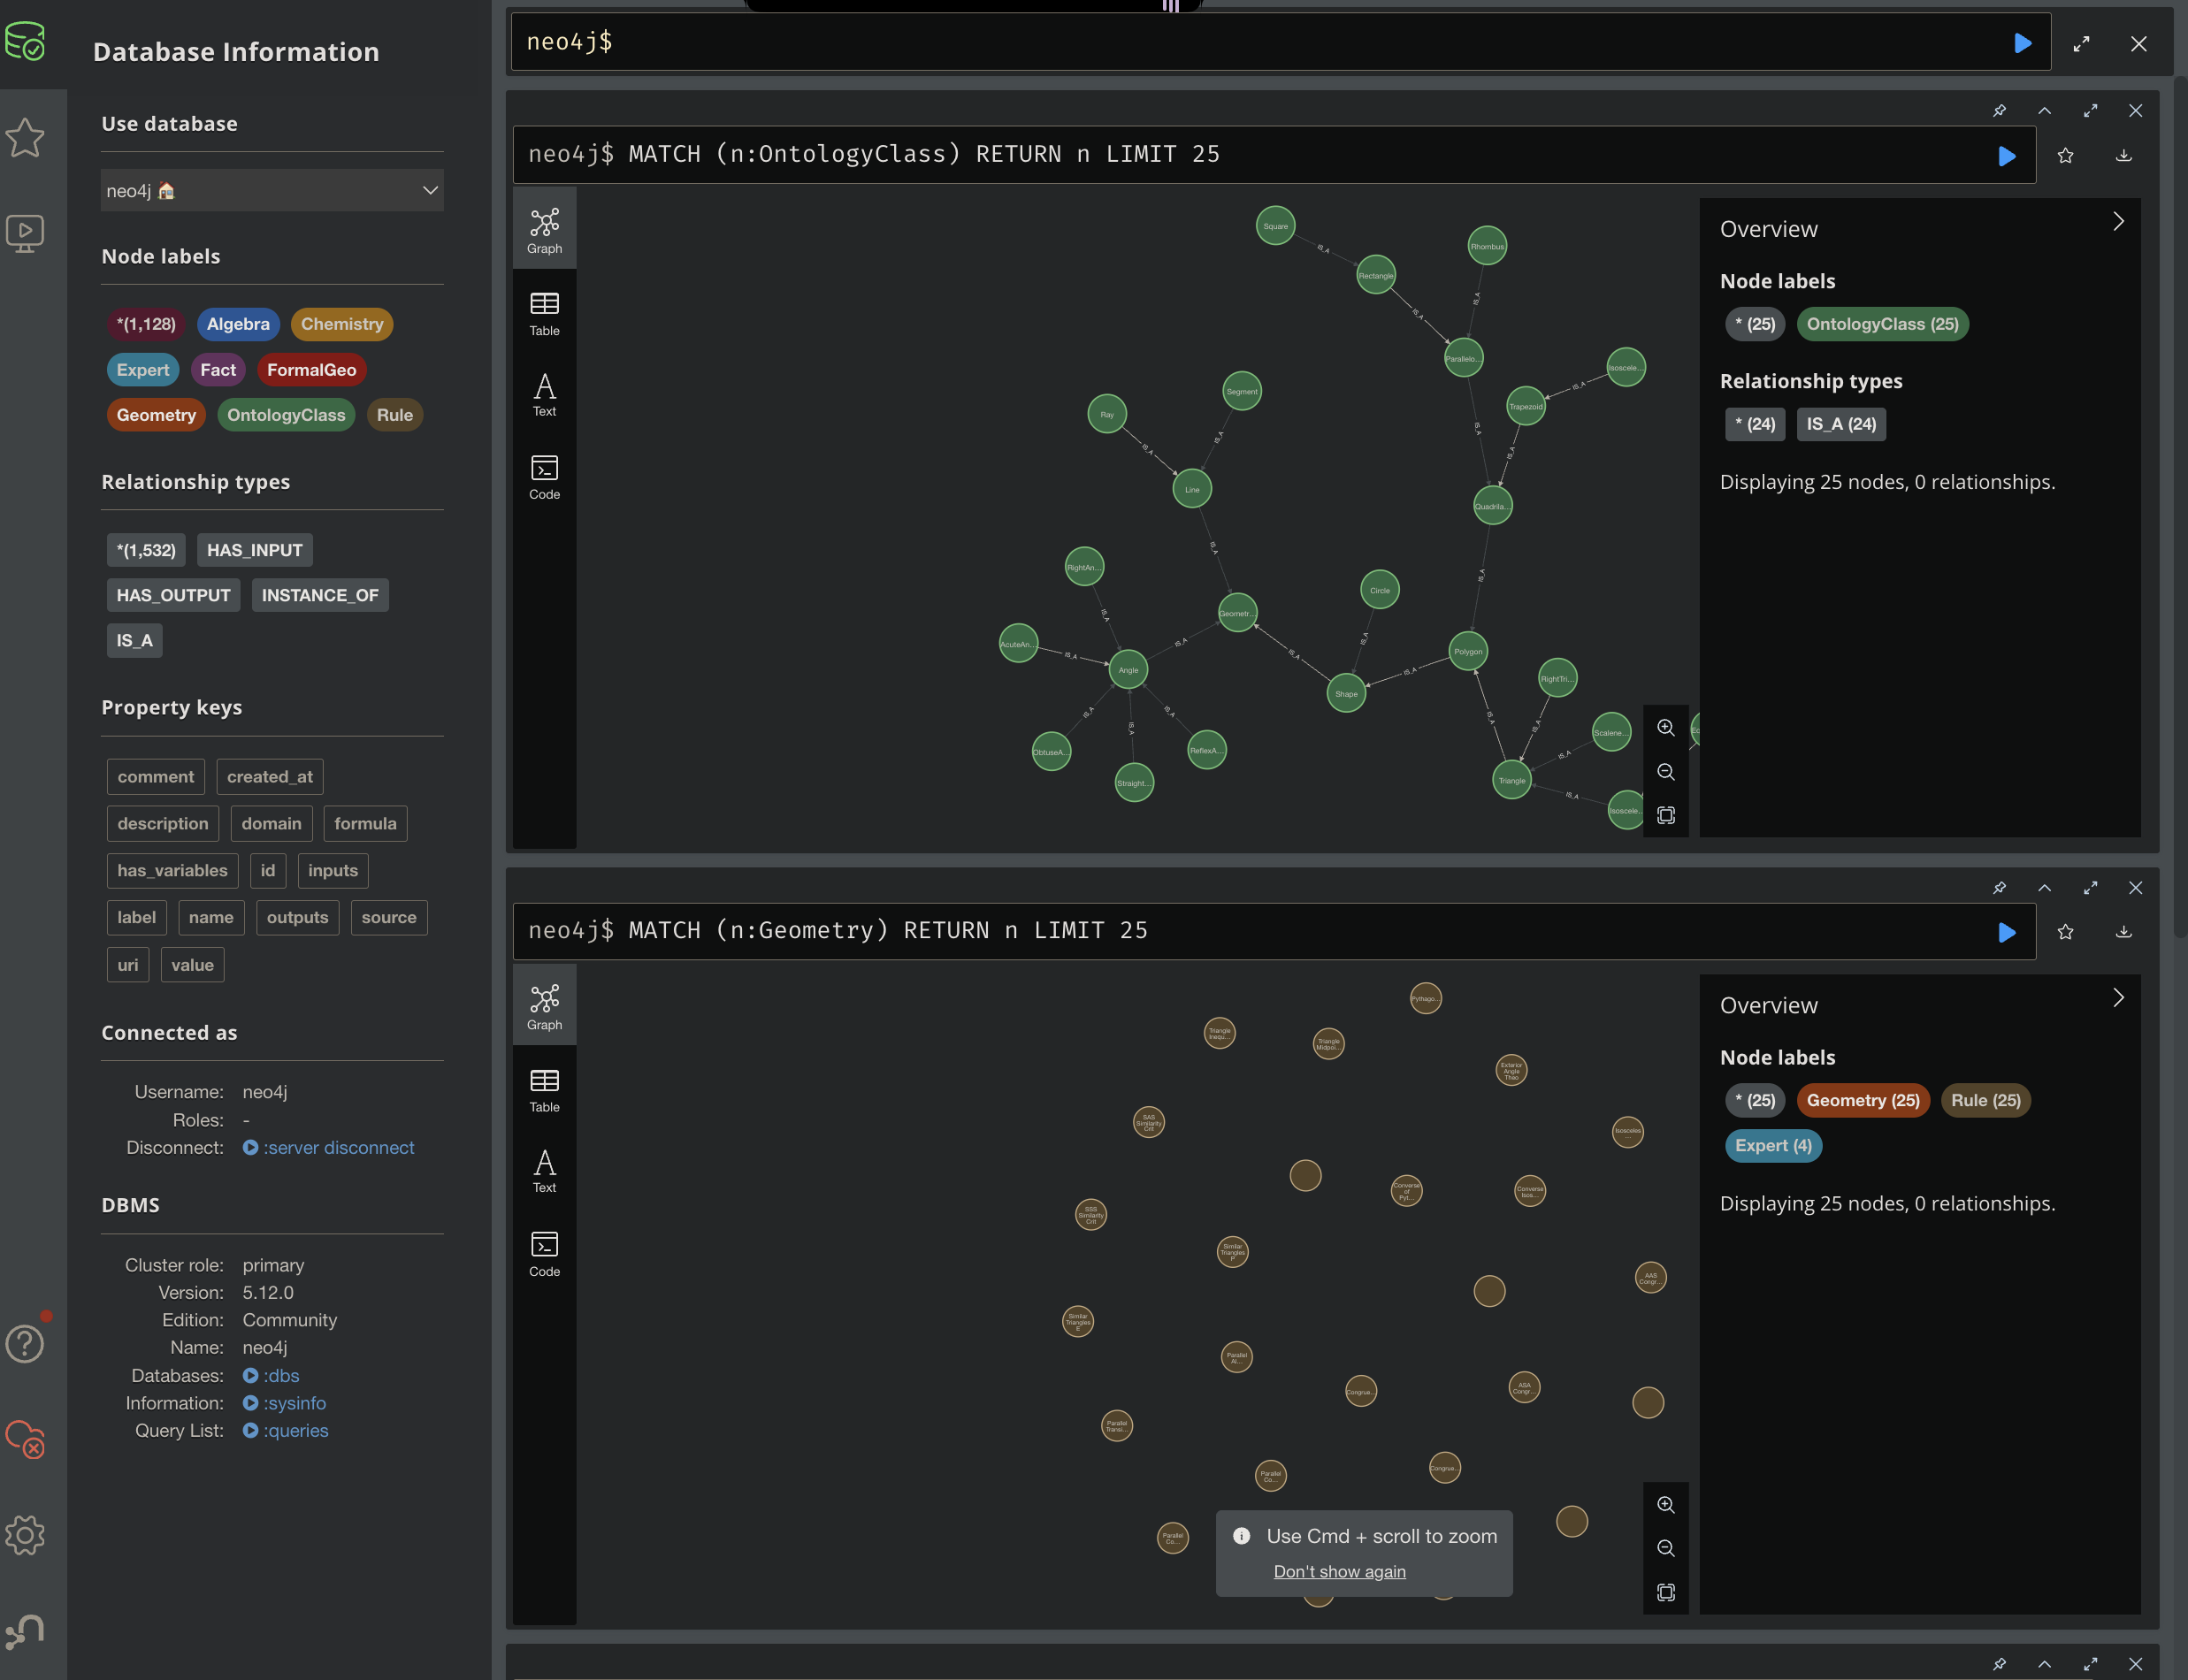
\includegraphics[width=\textwidth]{../assets/neo4j_full_ontology_1128_nodes.png}
    \caption{Thống kê toàn bộ Ontology trên Neo4j (1.128 nút, 1.532 quan hệ).}
    \label{fig:neo4j_ontology_stats}
\end{subfigure}
\hfill
\begin{subfigure}[b]{0.48\textwidth}
    \includegraphics[width=\textwidth]{../assets/neo4j_knowledge_base.png}
    \caption{Trực quan hóa mạng lưới kết nối giữa các định lý và tiên đề.}
    \label{fig:neo4j_graph_view}
\end{subfigure}
\caption{Cơ sở Tri thức Đồ thị Hình học Phẳng được xây dựng và truy vấn trên Neo4j.}
\label{fig:neo4j_full_kb}
\end{figure}

Như thể hiện trong Hình~\ref{fig:neo4j_ontology_stats}, cơ sở tri thức đã được nạp đầy đủ \textbf{1.128 nút} và \textbf{1.532 quan hệ}, bao quát toàn diện các nhánh tri thức:
\begin{itemize}
    \item \textbf{Nhóm Tiên đề Euclid Cơ bản}: Quan hệ cộng góc, cộng đoạn thẳng, góc đối đỉnh, góc so le trong, góc đồng vị, các trường hợp bằng nhau của tam giác ($c-c-c, c-g-c, g-c-g$).
    \item \textbf{Nhóm Định lý Tam giác \& Tứ giác}: Định lý Pythagore, Định lý Thales, đường trung bình, tính chất trọng tâm, trực tâm, tâm đường tròn nội/ngoại tiếp, tính chất hình thoi, hình bình hành, tứ giác nội tiếp.
    \item \textbf{Nhóm Định lý Đường tròn Nâng cao}: Góc nội tiếp, góc tạo bởi tiếp tuyến và dây cung, phương tích của một điểm đối với đường tròn (Định lý cát tuyến - tiếp tuyến $PT^2 = PA \cdot PB$, Định lý hai dây cung cắt nhau $PA \cdot PB = PC \cdot PD$).
    \item \textbf{Nhóm Định lý Olympic (IMO)}: Định lý Ptolemy cho tứ giác nội tiếp, Định lý Ceva, Định lý Menelaus, Định lý đường thẳng Simson, Định lý Varignon cho trung điểm tứ giác, Bổ đề điểm Nagel.
\end{itemize}

\section{Cơ sở Dữ liệu Vector Qdrant và Cơ chế GraphRAG}
Để giải quyết bài toán tìm kiếm định lý phù hợp từ ngôn ngữ tự nhiên hoặc từ tập sự kiện phức tạp mà không phụ thuộc vào chuỗi ký tự cứng nhắc (Exact Keyword Matching), hệ thống sử dụng \textbf{Qdrant Cloud Vector Database} làm động cơ tìm kiếm tương đồng ngữ nghĩa (Dense Semantic Search).

\begin{figure}[h!]
\centering
\begin{subfigure}[b]{0.48\textwidth}
    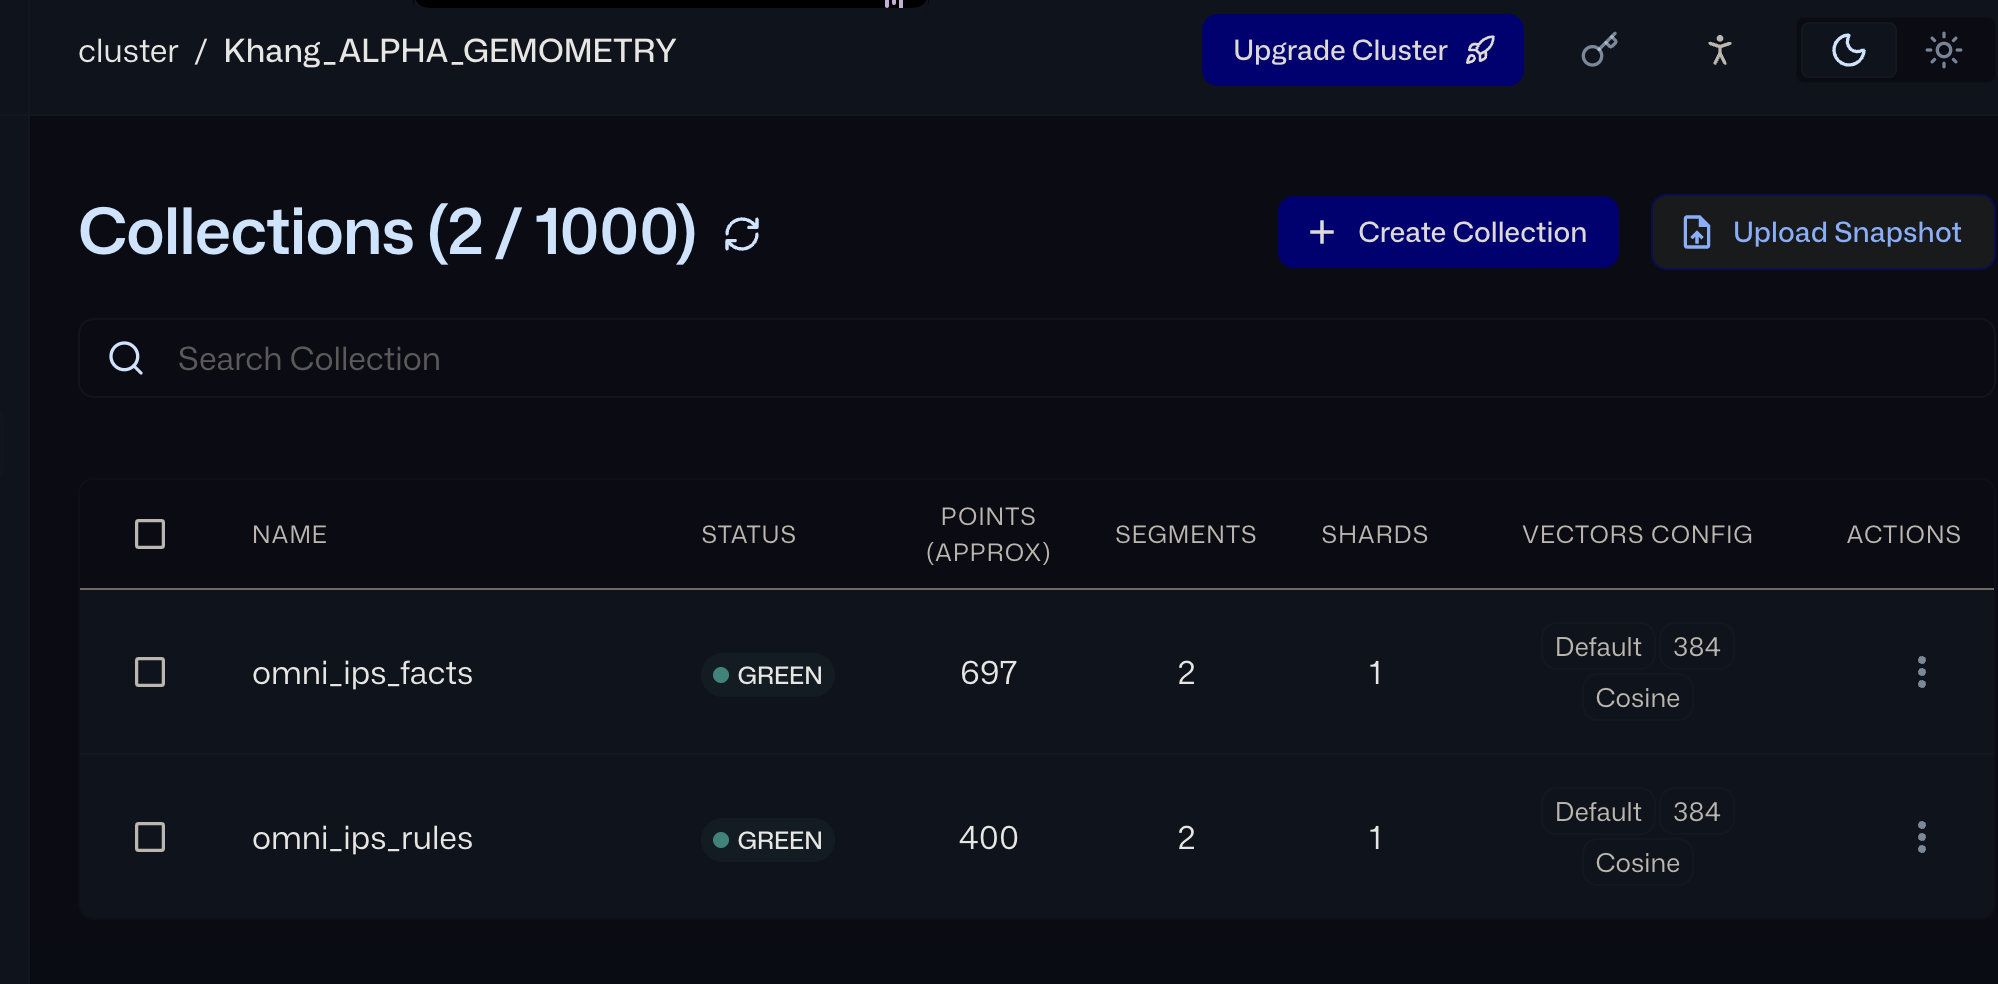
\includegraphics[width=\textwidth]{../assets/qdrant_collections_overview.png}
    \caption{Tổng quan các Collections được lập chỉ mục vector trên Qdrant.}
    \label{fig:qdrant_collections}
\end{subfigure}
\hfill
\begin{subfigure}[b]{0.48\textwidth}
    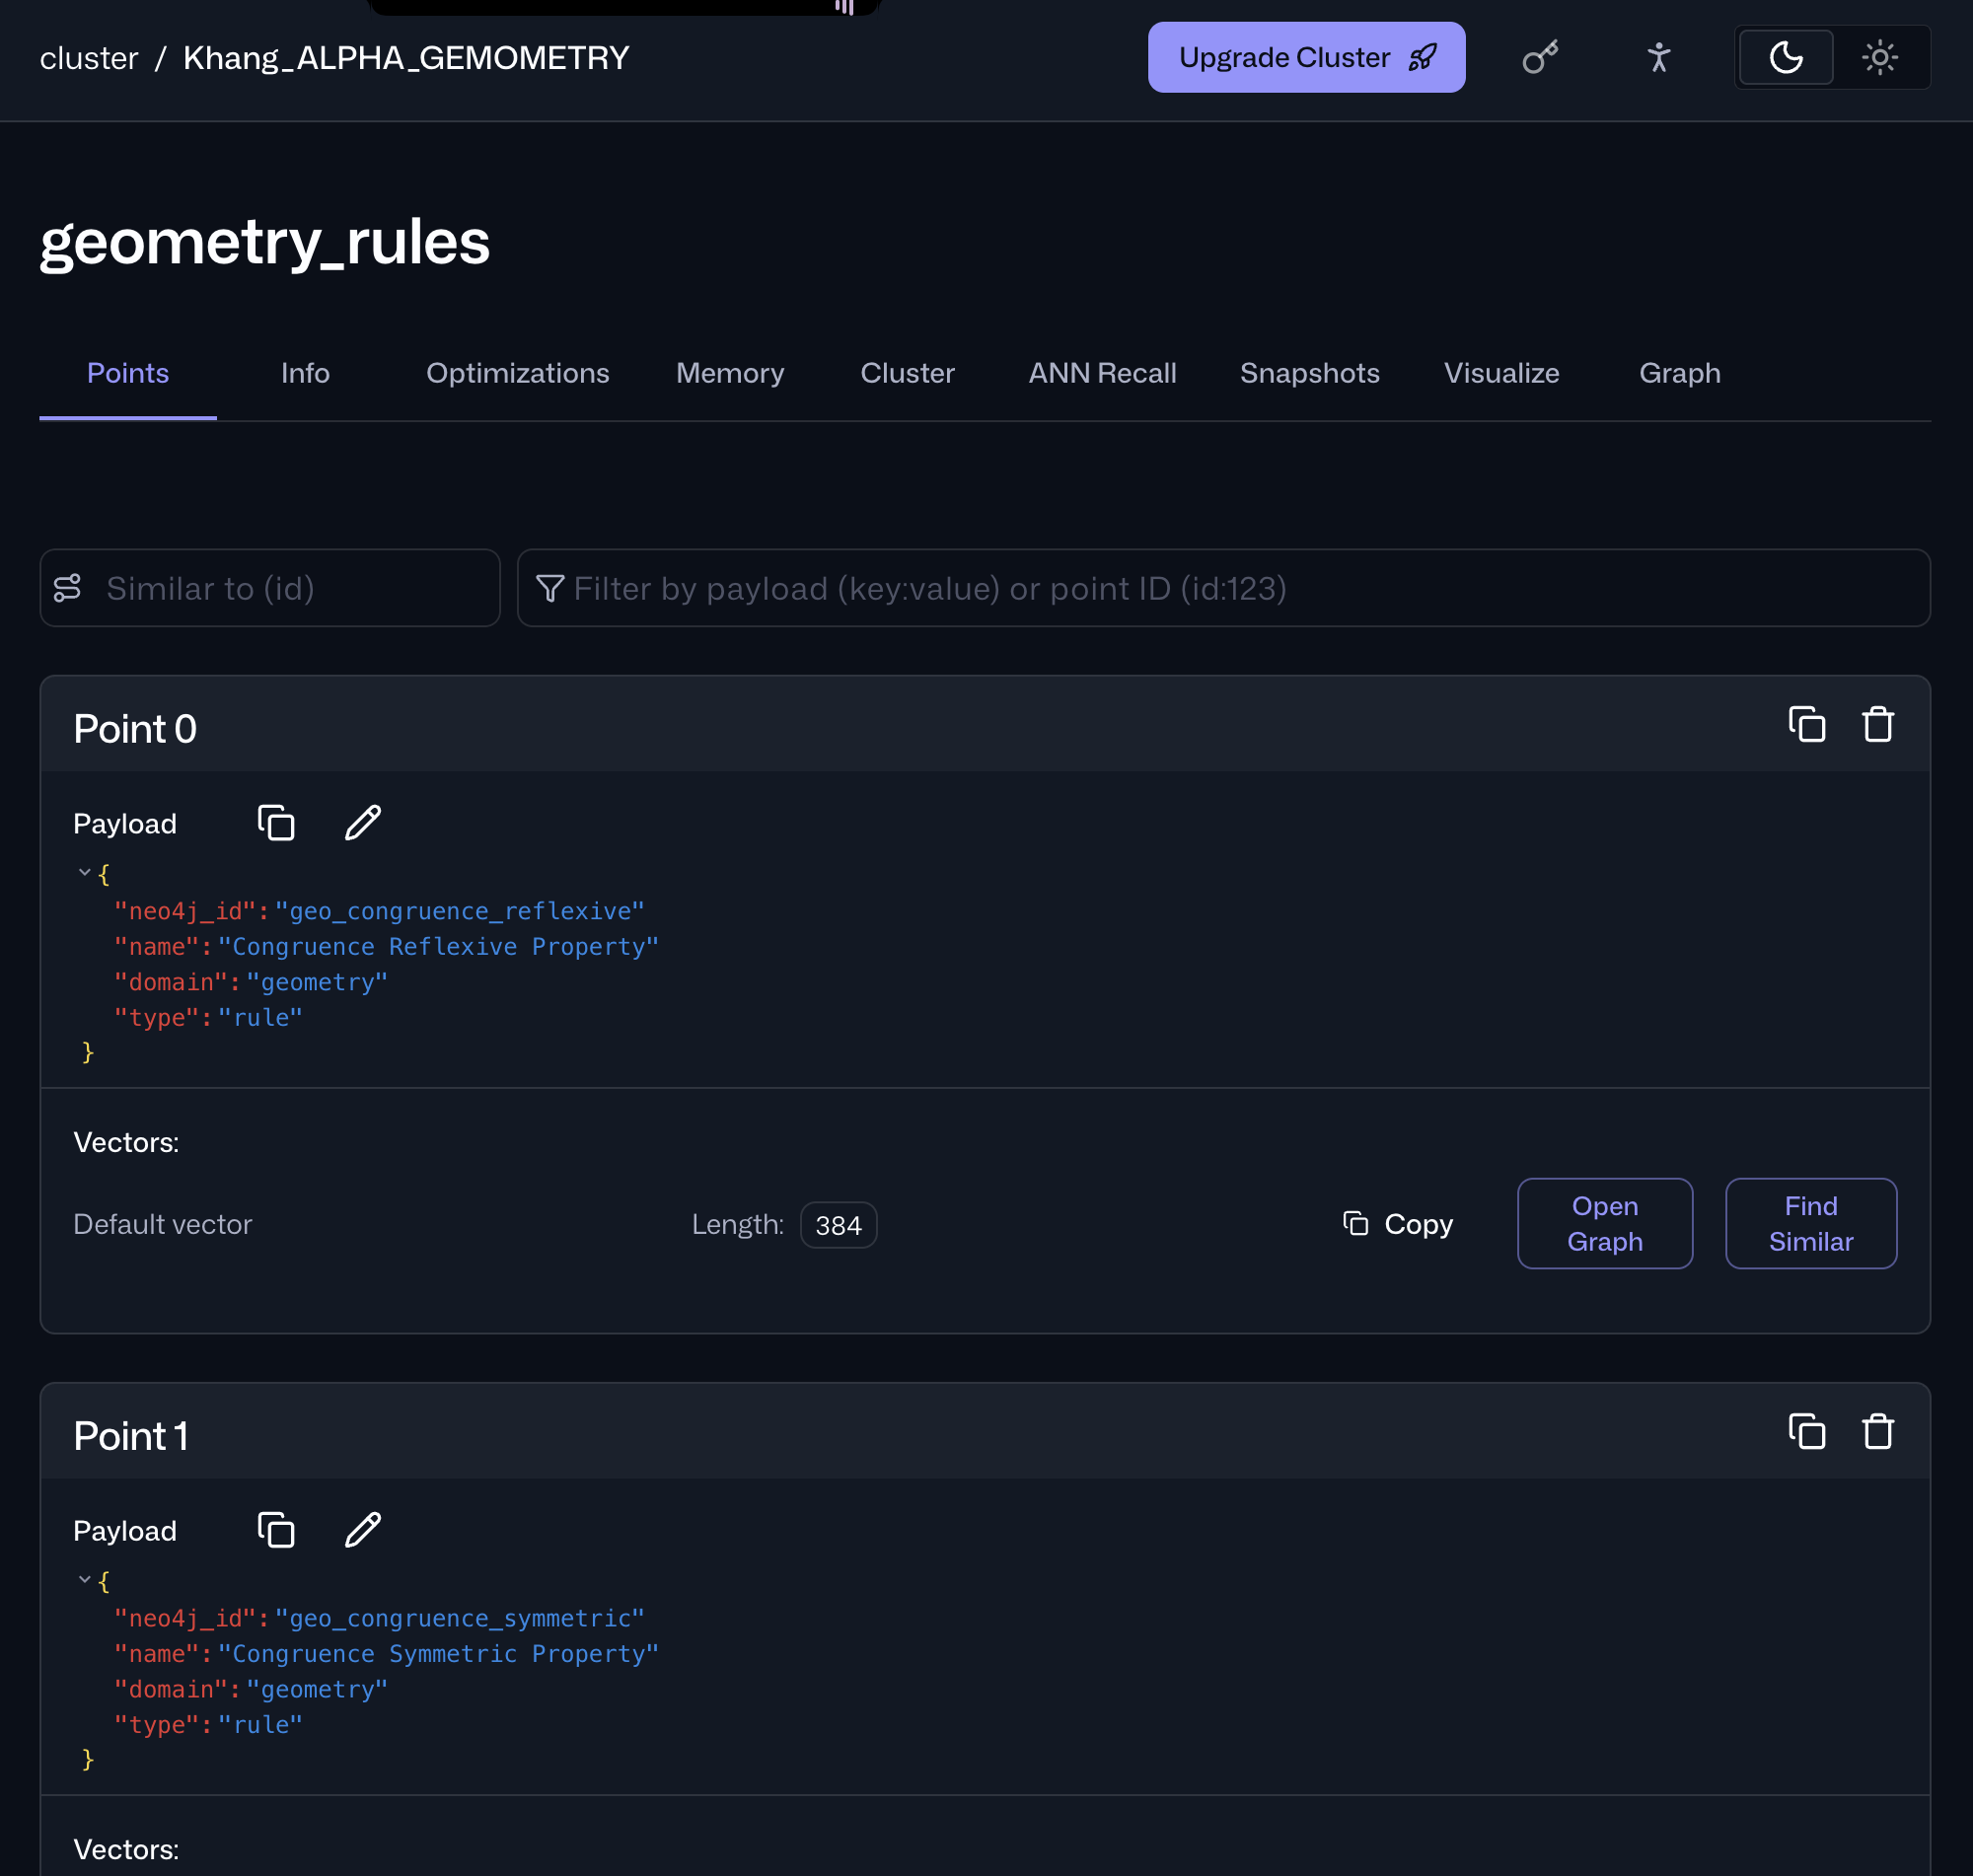
\includegraphics[width=\textwidth]{../assets/qdrant_rules_payload_detail.png}
    \caption{Cấu trúc Payload chi tiết của một định lý hình học trong Qdrant.}
    \label{fig:qdrant_rules_payload}
\end{subfigure}
\caption{Quản lý và lập chỉ mục không gian vector tri thức hình học trên Qdrant Cloud.}
\label{fig:qdrant_management}
\end{figure}

\subsection{Cấu trúc Chỉ mục Vector trong Qdrant}
Như minh họa trong Hình~\ref{fig:qdrant_collections}, hệ thống duy trì hai collection vector chính:
\begin{enumerate}
    \item \texttt{omni\_ips\_rules} (hoặc \texttt{geometry\_rules}): Lưu trữ các định lý và quy tắc suy diễn hình học. Mỗi vector đại diện cho mô tả ngữ nghĩa, công thức toán học và tiền đề của một luật. Payload chứa định danh Neo4j (\texttt{neo4j\_id}), mô tả và mã luật tương ứng (Hình~\ref{fig:qdrant_rules_payload}).
    \item \texttt{omni\_ips\_facts} (hoặc \texttt{geometry\_facts}): Lưu trữ các dạng biểu diễn vị từ thực tế của các sự kiện hình học, hỗ trợ ánh xạ nhanh các câu khẳng định tự nhiên sang vị từ chuẩn (Hình~\ref{fig:qdrant_facts_payload}).
\end{enumerate}

\begin{figure}[h!]
\centering
\begin{subfigure}[b]{0.48\textwidth}
    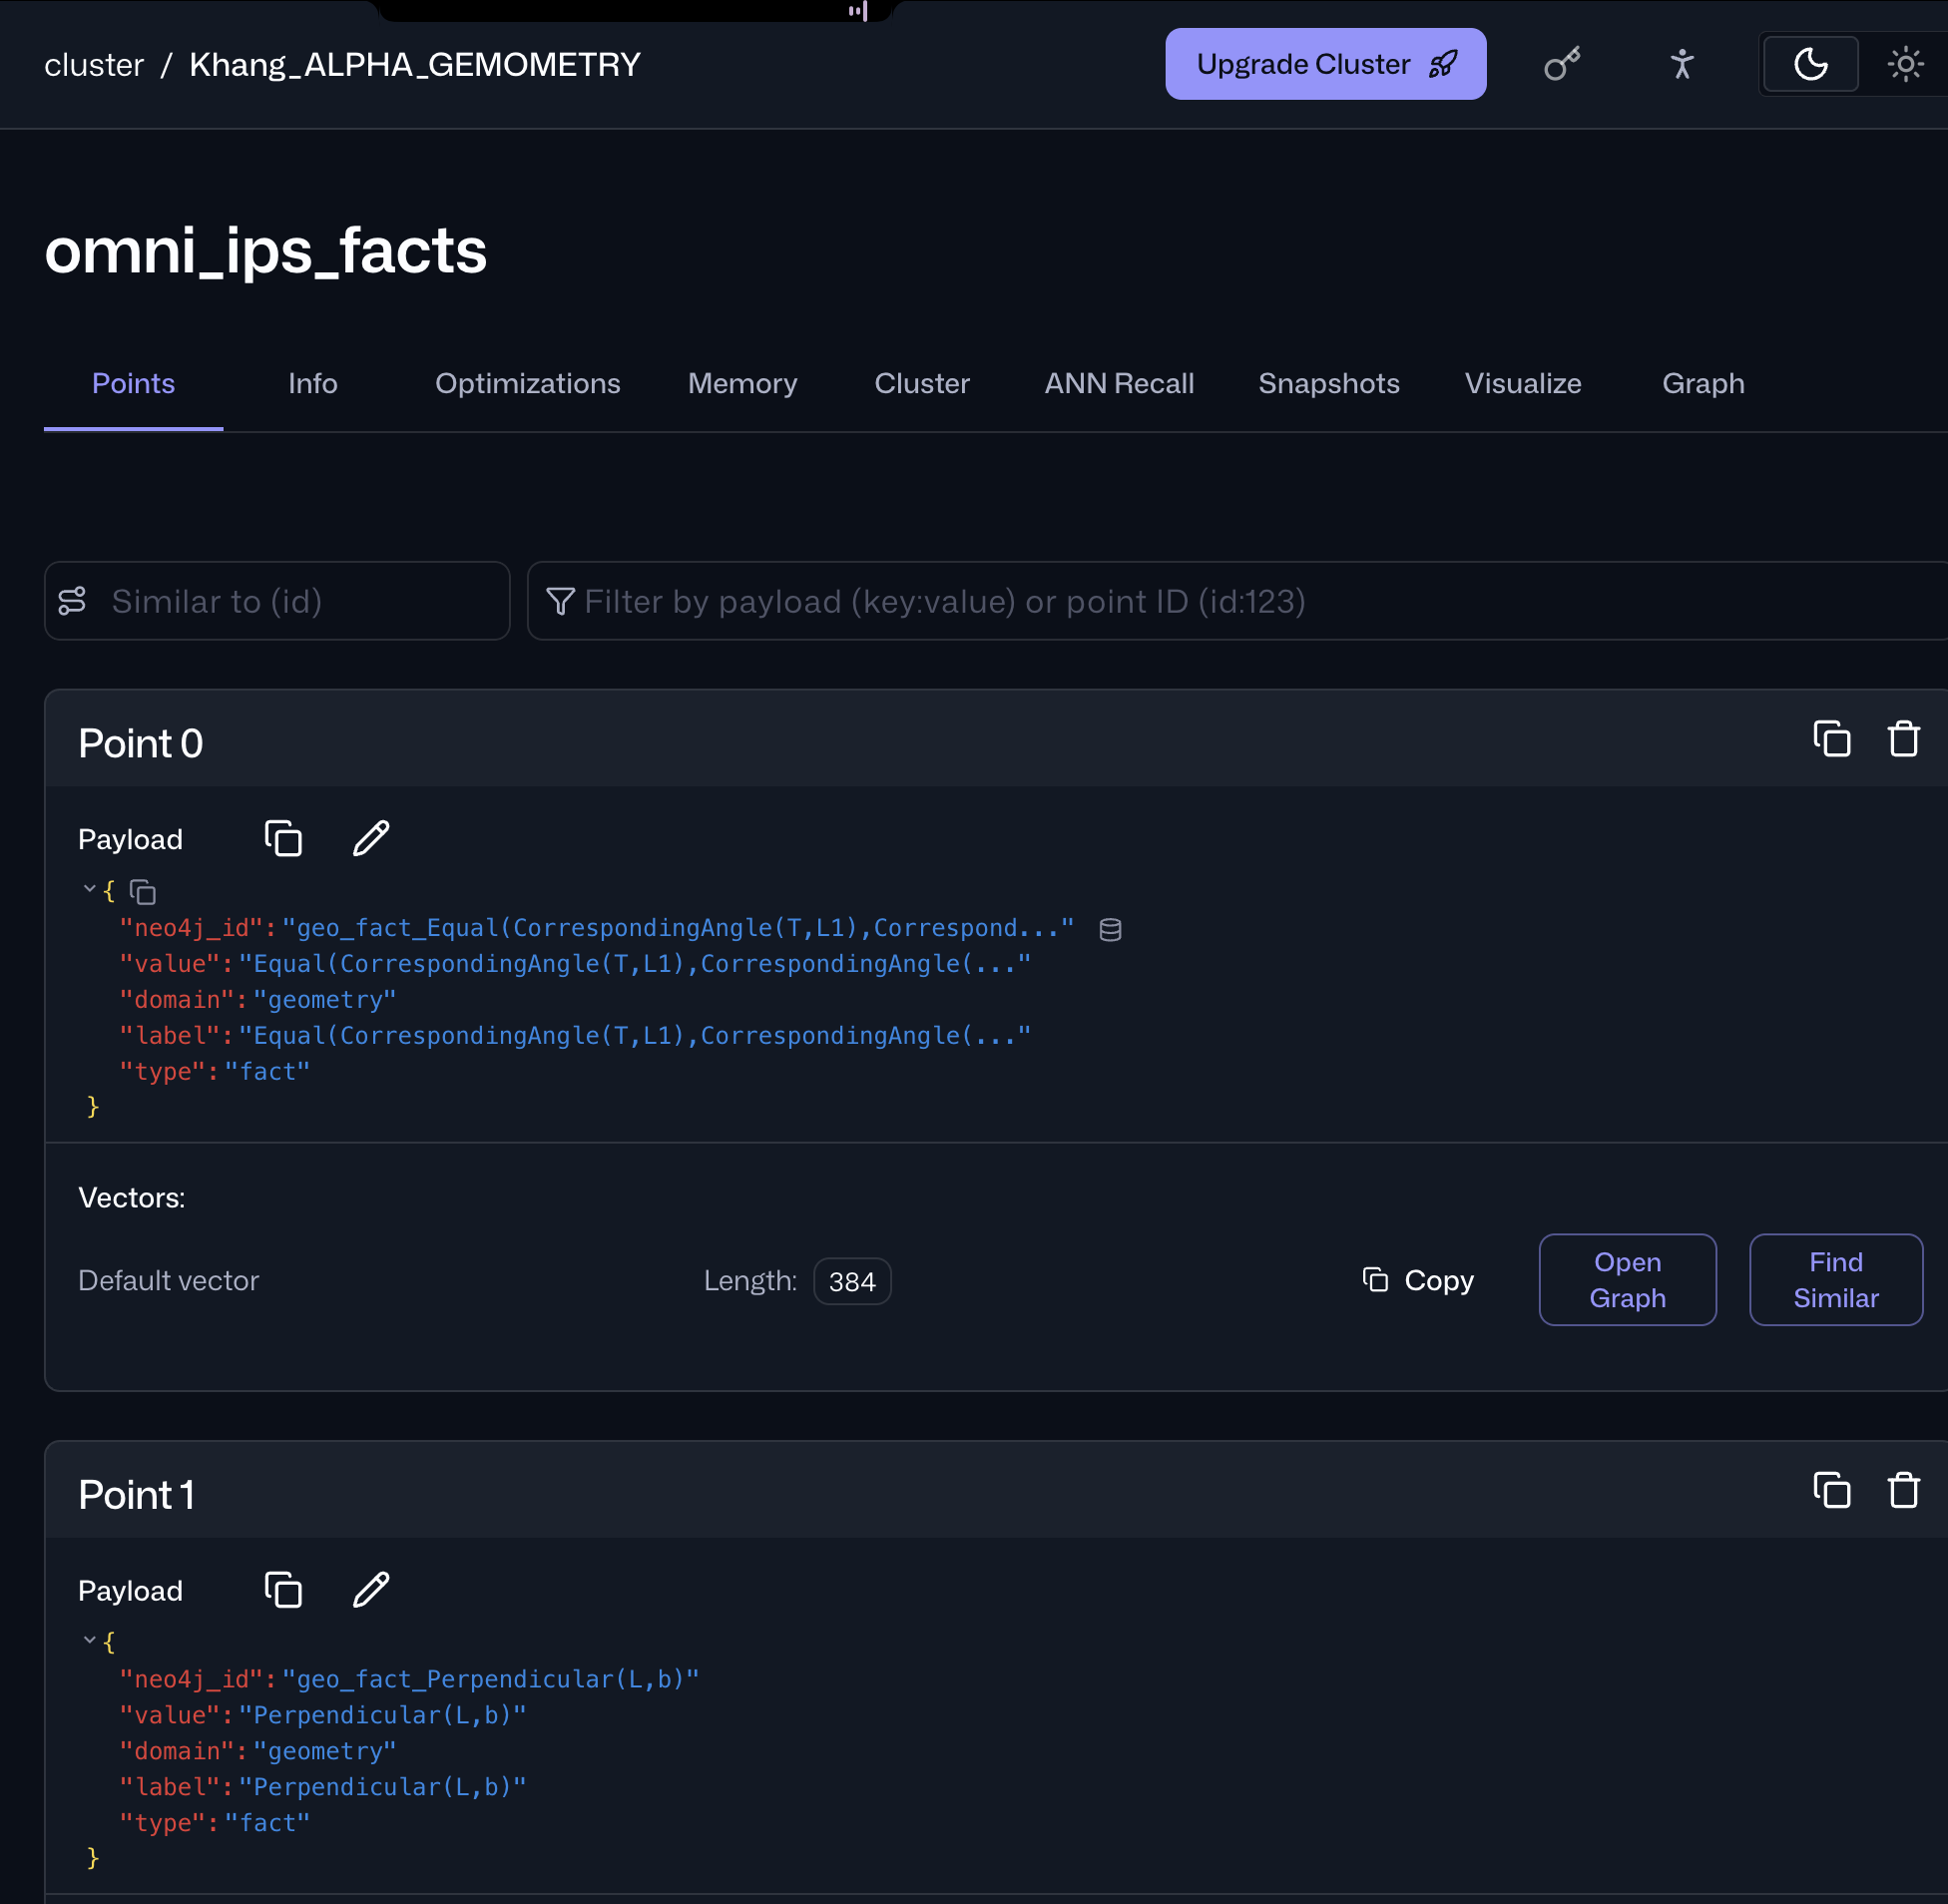
\includegraphics[width=\textwidth]{../assets/qdrant_facts_payload_detail.png}
    \caption{Payload vị từ sự kiện hình học trong \texttt{omni\_ips\_facts}.}
    \label{fig:qdrant_facts_payload}
\end{subfigure}
\hfill
\begin{subfigure}[b]{0.48\textwidth}
    \includegraphics[width=\textwidth]{../assets/qdrant_vector_db.png}
    \caption{Truy vấn tương đồng vector điểm sự kiện \texttt{Midpoint(N,AC)}.}
    \label{fig:qdrant_vector_search}
\end{subfigure}
\caption{Chi tiết lưu trữ sự kiện và không gian vector trên Qdrant.}
\label{fig:qdrant_details}
\end{figure}

\section{Bộ Định tuyến Neuro-Symbolic và Trích xuất Vị từ từ Đề bài}
Một mắt xích tối quan trọng trong hệ thống là quá trình chuyển đổi (Parsing) đề bài bài toán từ ngôn ngữ tự nhiên tiếng Việt (kèm theo mã công thức LaTeX) sang tập hợp các vị từ ban đầu (Initial Facts) và mục tiêu cần chứng minh (Goal).

\subsection{Quy trình Xử lý Vị từ Đa tầng (Multi-Stage Parsing Pipeline)}
\begin{enumerate}
    \item \textbf{Tầng 1: Bộ Tiền Xử lý và Làm sạch Toán học (\texttt{clean\_geometry\_query})}:
    Tự động chuẩn hóa các ký tự LaTeX dính liền hoặc biểu thức OCR lỗi từ việc copy-paste đề bài:
    $$\text{((O))} \longrightarrow \text{O}, \quad \text{\textbackslash cdot} \longrightarrow *, \quad \text{\textbackslash perp} \longrightarrow \text{vuông góc}, \quad \text{đoạn thẳng (MA, MB)} \longrightarrow \text{MA, MB}$$
    
    \item \textbf{Tầng 2: Direct JSON Schema Prompting qua LLM}:
    Thay vì sử dụng Function Calling (vốn dễ gây ra lỗi $400\ \text{tool\_use\_failed}$ trên các endpoint suy luận), hệ thống truyền trực tiếp lược đồ JSON nghiêm ngặt vào \texttt{SystemMessage} của mô hình ngôn ngữ lớn (Llama-3.3-70B / DeepSeek / GPT-OSS-120B). Đầu ra được trích xuất bằng regex JSON block an toàn với thời gian phản hồi cực nhanh ($< 1.8\text{s}$).

    \item \textbf{Tầng 3: Bộ Phân tích Dự phòng Offline (Regex Fallback Parser)}:
    Trong trường hợp mất kết nối mạng hoặc LLM quá tải, bộ phân tích Regex cục bộ sẽ tự động quét các từ khóa hình học đặc thù để trích xuất đầy đủ các vị từ: tam giác vuông, tiếp tuyến, cát tuyến, trung điểm, đường cao và tứ giác nội tiếp.
\end{enumerate}

% ==============================================================================
% CHƯƠNG 3: KIẾN TRÚC SUY DIỄN NEURO-SYMBOLIC, ĐẠI SỐ HÓA VÀ DỰNG HÌNH PHỤ
% ==============================================================================

\chapter{KIẾN TRÚC SUY DIỄN NEURO-SYMBOLIC, ĐẠI SỐ HÓA VÀ DỰNG HÌNH PHỤ}
\label{chap:reasoning}

\section{Động cơ Suy diễn Tiến Ký hiệu (Forward Chaining Deduction Engine)}
Cốt lõi của cỗ máy chứng minh hình thức là \textbf{Động cơ Suy diễn Tiến (Forward Chaining Deduction Engine)}, hoạt động trên Bộ nhớ Làm việc ($\mathcal{WM}$ -- Working Memory).

\subsection{Cấu trúc Tập Luật và Hợp giải Vị từ (Unification)}
Mỗi luật suy diễn hình học $r \in \mathcal{R}$ được định nghĩa bởi cặp tiền đề và kết luận:
\begin{equation}
    r = \langle \text{Inputs}(r), \text{Outputs}(r) \rangle
\end{equation}
trong đó $\text{Inputs}(r) = \{p_1(?x_1, \dots), \dots, p_k(?x_k, \dots)\}$ là tập các mẫu vị từ chứa biến (bắt đầu bằng dấu \texttt{?}), và $\text{Outputs}(r) = \{q_1(?x_1, \dots), \dots, q_m(?x_m, \dots)\}$ là các sự kiện suy ra sau khi thế biến.

\subsection{Chuẩn hóa Đồng nhất và Quan hệ Tương đương (Canonical Equivalence)}
Trong hình học, một đối tượng có thể được biểu diễn qua nhiều hoán vị đỉnh có tính chất tương đương (ví dụ: đoạn thẳng $AB \equiv BA$, góc $\angle ABC \equiv \angle CBA$, tam giác $\triangle ABC \equiv \triangle BCA$). Nếu không chuẩn hóa, bộ nhớ làm việc sẽ bị bùng nổ tổ hợp do lưu trữ trùng lặp.

Hệ thống định nghĩa hàm chuẩn hóa chính quy $\text{Canonical}(P)$ cho mọi vị từ:
\begin{itemize}
    \item Với đoạn thẳng: $\text{Canonical}(\text{Segment}(A, B)) = \text{Segment}(\min(A, B), \max(A, B))$.
    \item Với góc: $\text{Canonical}(\text{Angle}(A, B, C)) = \text{Angle}(\min(A, C), B, \max(A, C))$.
    \item Với đường thẳng song song:
    $$\text{Parallel}(AB, CD) \equiv \text{Parallel}(CD, AB) \equiv \text{Parallel}(BA, CD) \equiv \text{Parallel}(DC, AB)$$
\end{itemize}

\begin{algorithm}[h!]
\caption{Thuật toán Suy diễn Tiến Hình học Phẳng (Forward Chaining with Canonical Normalization)}
\label{alg:forward_chaining}
\begin{algorithmic}[1]
\Require Tập sự kiện ban đầu $\mathcal{F}_0$, Tập luật $\mathcal{R}$, Vị từ mục tiêu $\mathcal{G}$, Ngưỡng lặp cực đại $M$
\Ensure Trạng thái chứng minh (\texttt{True/False}), Dấu vết suy diễn $\mathcal{T}$
\State $\mathcal{WM} \leftarrow \bigcup_{f \in \mathcal{F}_0} \text{Canonical}(f)$
\State $\mathcal{T} \leftarrow []$
\State $step \leftarrow 0$
\While{$step < M$}
    \If{$\text{CheckGoal}(\mathcal{WM}, \mathcal{G})$}
        \State \Return \textbf{True}, $\mathcal{T}$ \Comment{Đã đạt được mục tiêu chứng minh}
    \EndIf
    \State $new\_facts \leftarrow \emptyset$
    \For{mỗi luật $r \in \mathcal{R}$}
        \State $bindings \leftarrow \text{UnifyMultiple}(\text{Inputs}(r), \mathcal{WM})$
        \For{mỗi phép thế $\theta \in bindings$}
            \State $conclusions \leftarrow \text{Substitute}(\text{Outputs}(r), \theta)$
            \For{mỗi $c \in conclusions$}
                \State $c_{can} \leftarrow \text{Canonical}(c)$
                \If{$c_{can} \notin \mathcal{WM}$}
                    \State $new\_facts \leftarrow new\_facts \cup \{c_{can}\}$
                    \State $\mathcal{T} \leftarrow \mathcal{T} \cup \{\langle r, \theta, c_{can} \rangle\}$
                \EndIf
            \EndFor
        \EndFor
    \EndFor
    \If{$new\_facts = \emptyset$}
        \State \textbf{break} \Comment{Đạt trạng thái bão hòa (Bế tắc)}
    \EndIf
    \State $\mathcal{WM} \leftarrow \mathcal{WM} \cup new\_facts$
    \State $step \leftarrow step + 1$
\EndWhile
\State \Return \textbf{False}, $\mathcal{T}$
\end{algorithmic}
\end{algorithm}

\section{Động cơ Suy diễn Đại số SymPy AR (Algebraic Reasoning)}
Các quan hệ về góc (Angle Chasing) và độ dài đoạn thẳng thường đòi hỏi các phép biến đổi phương trình liên tục mà suy diễn vị từ rời rạc khó có thể bao quát hết mọi phép biến đổi tương đương. Do đó, hệ thống tích hợp động cơ đại số hình thức \textbf{SymPy AR} chạy song song với động cơ suy diễn tiến.

\subsection{Cơ chế Hoạt động của SymPy AR}
\begin{enumerate}
    \item \textbf{Đại số hóa Vị từ (Equation Extraction)}: Chuyển các vị từ cộng góc $\text{Equal}(\text{Add}(\text{Angle}(A), \text{Angle}(B)), \text{Angle}(C))$ thành các phương trình đại số dạng biểu thức tượng trưng SymPy:
    $$\text{Equal}(\text{Add}(\text{Angle}(A), \text{Angle}(B), \text{Angle}(C)), 180) \implies \theta_A + \theta_B + \theta_C - 180 = 0$$
    \item \textbf{Khử Ẩn số và Giải Hệ Phương trình (Elimination \& Linear Solving)}: Sử dụng ma trận giải hệ phương trình tuyến tính hoặc phương pháp phần bù (Elimination Method) của SymPy để giải tìm giá trị ẩn số của mục tiêu:
    $$\theta_C = 180 - \theta_A - \theta_B = 180 - 60 - 70 = 50^\circ$$
    \item \textbf{Tái tạo Vị từ (Fact Injection)}: Khi một giá trị đại số mới được chứng minh, nó được đóng gói lại thành vị từ chính quy $\text{Equal}(\text{Angle}(C), 50)$ và nạp ngược trở lại $\mathcal{WM}$.
\end{enumerate}

\section{Tác tử Sinh Hình phụ Neuro-Symbolic (Auxiliary Construction Agent)}
Trong các bài toán hình học nâng cao (đặc biệt là đề thi học sinh giỏi và Olympic IMO), nhiều định lý không thể chứng minh trực tiếp nếu chỉ dựa trên các đối tượng ban đầu. Cần phải kẻ thêm các \textbf{đối tượng hình học phụ (Auxiliary Elements)}.

\begin{figure}[h!]
\centering
\begin{tikzpicture}[scale=0.88, transform shape]
    % Left column
    \node [base, fill=blue!12, draw=blue!85!black, minimum width=3.8cm, minimum height=1.3cm, inner sep=6pt] (start) at (-4.5, 2.2) {
        \textbf{Tập sự kiện ban đầu $\mathcal{F}_0$}\\[3pt]
        {\scriptsize (Working Memory $\mathcal{WM}$)}
    };
    
    \node [agent, fill=purple!15, draw=purple!85!black, minimum width=3.8cm, minimum height=1.3cm, inner sep=6pt] (aux) at (-4.5, -2.4) {
        \textbf{Auxiliary Agent (LLM)}\\[3pt]
        {\scriptsize Phân tích Gap \& Dựng hình phụ}
    };

    % Center column
    \node [process, fill=green!15, draw=green!65!black, minimum width=4.5cm, minimum height=1.3cm, inner sep=6pt] (forward) at (1.0, 2.2) {
        \textbf{Forward Deduction Engine}\\[3pt]
        {\scriptsize (Luật vị từ + FormalGeo)}
    };
    
    \node [process, fill=yellow!18, draw=orange!75!black, minimum width=4.5cm, minimum height=1.3cm, inner sep=6pt] (sympy) at (1.0, -0.1) {
        \textbf{SymPy AR Engine}\\[3pt]
        {\scriptsize (Đại số hóa góc \& đoạn thẳng)}
    };
    
    \node [decision, fill=yellow!18, draw=orange!85!black, minimum width=3.0cm, minimum height=1.4cm] (goal_check) at (1.0, -2.4) {
        \textbf{Đạt}\\[1pt]\textbf{Goal?}
    };

    % Right column
    \node [base, fill=teal!18, draw=teal!85!black, minimum width=3.6cm, minimum height=1.3cm, inner sep=6pt] (done) at (6.2, -2.4) {
        \textbf{Hoàn thành! \faCheckCircle}\\[3pt]
        {\scriptsize Xuất lời giải logic}
    };

    % Arrows with clear, non-overlapping labels
    \draw [arrow] (start) -- (forward);
    \draw [arrow] (forward) -- (sympy);
    \draw [arrow] (sympy) -- (goal_check);
    \draw [arrow] (goal_check.east) -- node[above=3pt, font=\bfseries\small, text=teal!85!black] {Có} (done.west);
    \draw [arrow] (goal_check.west) -- node[above=3pt, font=\bfseries\small, text=red!85!black] {Bế tắc} (aux.east);
    \draw [arrow] (aux.north) -- node[left=4pt, font=\itshape\footnotesize, text=purple!90!black, align=right] {Nạp hình phụ\\vào $\mathcal{WM}$} (start.south);
\end{tikzpicture}
\caption{Quy trình phối hợp toàn diện giữa Suy diễn tiến, SymPy AR và Tác tử Sinh hình phụ.}
\label{fig:full_reasoning_flow}
\end{figure}

\subsection{Chiến lược Đề xuất Hình phụ}
Khi cỗ máy suy diễn đạt điểm bất động mà chưa đạt mục tiêu, \textbf{Tác tử Bổ trợ Hình phụ (Auxiliary Agent)} được kích hoạt:
\begin{enumerate}
    \item \textbf{Nhận diện Khoảng trống Chứng minh (Gap Analysis)}: So sánh tập sự kiện hiện có với cấu trúc vị từ của mục tiêu (ví dụ: mục tiêu yêu cầu chứng minh $\text{CyclicQuadrilateral}$, nhưng hiện chưa có đường tròn ngoại tiếp).
    \item \textbf{Đề xuất Mẫu Hình phụ Hợp lệ}:
    \begin{itemize}
        \item Dựng đường kính hoặc tâm đường tròn ngoại tiếp: $\text{Circumcircle}(\text{Circle}(O), \text{Triangle}(A, B, C))$.
        \item Lấy trung điểm đoạn thẳng: $\text{Midpoint}(M, AB)$.
        \item Dựng đường cao hoặc đường vuông góc: $\text{Perpendicular}(AH, BC)$.
        \item Nối hai đỉnh chưa liên kết để tạo tam giác đồng dạng.
    \end{itemize}
\end{enumerate}

% ==============================================================================
% CHƯƠNG 4: HIỆN THỰC HÓA HỆ THỐNG, GIAO DIỆN SƯ PHẠM VÀ THỰC NGHIỆM ĐÁNH GIÁ
% ==============================================================================

\chapter{HIỆN THỰC HÓA HỆ THỐNG, GIAO DIỆN SƯ PHẠM VÀ THỰC NGHIỆM ĐÁNH GIÁ}
\label{chap:implementation}

\section{Kiến trúc Phần mềm và Triển khai Microservices}
Toàn bộ hệ thống được thiết kế theo kiến trúc Microservices hiện đại, phân tách độc lập giữa tầng lưu trữ tri thức, tầng tính toán suy diễn và tầng giao diện người dùng.

\begin{figure}[h!]
\centering
\begin{tikzpicture}[scale=0.95, transform shape]
    % Tier 1: Frontend
    \node [base, fill=teal!15, draw=teal!80!black, text width=5.2cm] (frontend) at (0, 3.2) {
        \textbf{Frontend Presentation Layer}\\[2pt]
        {\scriptsize \faDesktop\ Streamlit UI (Port 8501)}\\[1pt]
        {\scriptsize Giao diện giải toán, nhập đề bài \& Stream sư phạm}
    };

    % Tier 2: Backend
    \node [process, fill=blue!15, draw=blue!85!black, text width=5.6cm] (backend) at (0, 1.0) {
        \textbf{Backend Inference Core \& Gateway}\\[2pt]
        {\scriptsize \faServer\ FastAPI Service (Port 8080)}\\[1pt]
        {\scriptsize Forward Chaining + SymPy AR + GraphRAG Router}
    };

    % Tier 3: Databases
    \node [database, fill=orange!12, draw=orange!85!black, text width=3.4cm] (neo4j) at (-3.4, -1.6) {
        \textbf{Neo4j Graph DB}\\[2pt]
        {\scriptsize \faProjectDiagram\ Bolt: 7687, HTTP: 7474}\\[1pt]
        {\scriptsize 1.128 Nodes, 1.532 Rel}
    };

    \node [database, fill=orange!12, draw=orange!85!black, text width=3.4cm] (qdrant) at (3.4, -1.6) {
        \textbf{Qdrant Vector DB}\\[2pt]
        {\scriptsize \faCloud\ Port 6333 / Cloud}\\[1pt]
        {\scriptsize Lập chỉ mục Rules \& Facts}
    };

    % Connecting Arrows
    \draw [arrow, <->] (frontend) -- node[right=4pt, font=\footnotesize\bfseries, text=blue!85!black] {HTTP / REST \& SSE} (backend);
    \draw [arrow, <->] (backend.215) -- node[above left=2pt, font=\footnotesize\bfseries, text=teal!85!black] {Cypher Bolt} (neo4j.north);
    \draw [arrow, <->] (backend.325) -- node[above right=2pt, font=\footnotesize\bfseries, text=orange!95!black] {gRPC / REST} (qdrant.north);
\end{tikzpicture}
\caption{Sơ đồ kiến trúc Microservices Docker phân tầng của hệ thống AlphaGeometry-IMO.}
\label{fig:system_architecture}
\end{figure}

\subsection{Chi tiết các Service trong Docker Compose}
\begin{itemize}
    \item \texttt{geo\_ips\_backend}: Chứa toàn bộ lõi suy diễn hình học, bộ định tuyến vị từ GraphRAG, động cơ SymPy AR, các endpoint giải toán (\texttt{/api/solve}, \texttt{/geo/solve}) và endpoint truyền luồng sư phạm (\texttt{/api/explain/stream}).
    \item \texttt{geo\_ips\_frontend}: Xây dựng bằng Streamlit, kết nối trực tiếp với backend qua API RESTful, hỗ trợ hiển thị công thức LaTeX mượt mà, sơ đồ suy diễn từng bước và bảng điều khiển trực quan.
    \item \texttt{geo\_ips\_neo4j}: Cơ sở dữ liệu đồ thị Neo4j 5.12 lưu trữ toàn bộ ontology và mạng lưới định lý hình học.
    \item \textbf{Qdrant Cloud}: Cụm cơ sở dữ liệu vector trên đám mây lưu trữ vector embedding đa chiều của các định lý và tiên đề.
\end{itemize}

\begin{figure}[h!]
\centering
\includegraphics[width=0.85\textwidth]{../assets/demo_Pythagore_2.png}
\caption{Giao diện chính của hệ thống xác nhận trạng thái trực tuyến của Backend, Neo4j và Qdrant.}
\label{fig:demo_ui_status}
\end{figure}

\section{Giao diện Sư phạm và Khả năng Giải thích Trực quan}
Một trong những mục tiêu quan trọng nhất của đề tài là xây dựng một cỗ máy giải toán \textit{"như một người bạn hướng dẫn"}, không chỉ trả về các ký hiệu logic khô khan mà phải xuất ra lời giải sư phạm hoàn chỉnh bằng tiếng Việt, có bố cục rõ ràng, lập luận chặt chẽ và công thức toán học chuẩn xác.

\begin{figure}[h!]
\centering
\begin{subfigure}[b]{0.48\textwidth}
    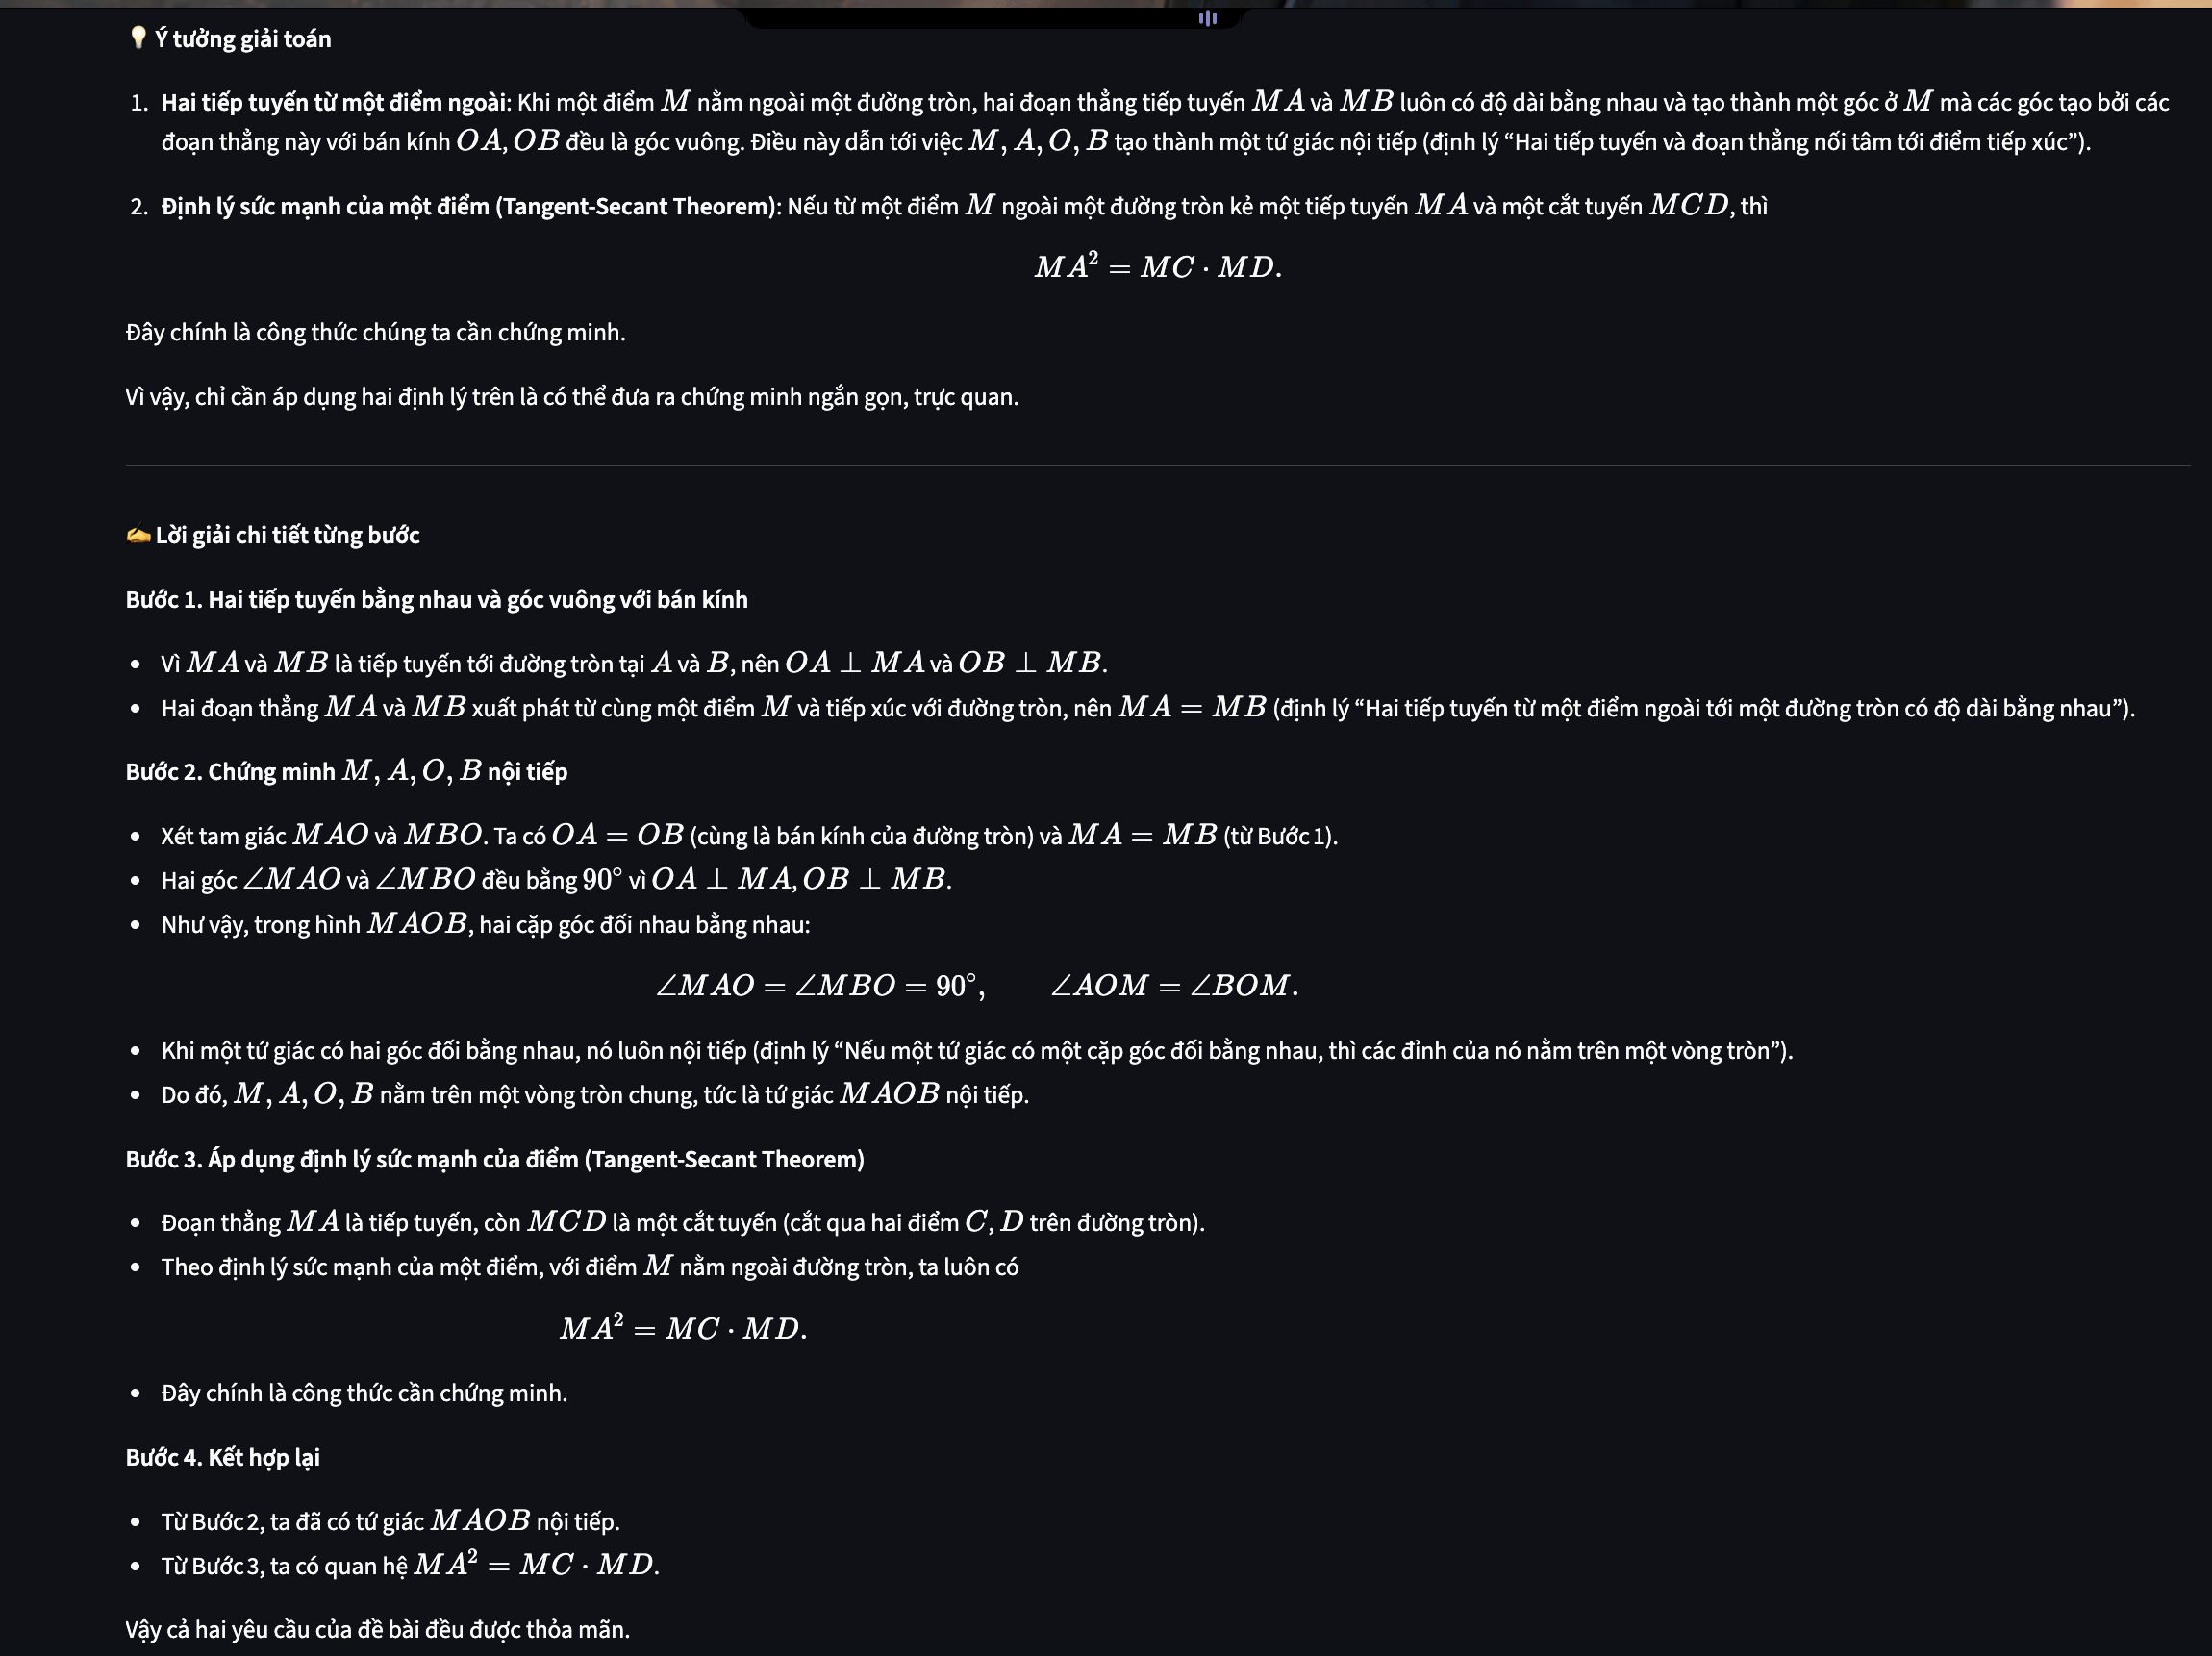
\includegraphics[width=\textwidth]{../assets/demo_pedagogical_explanation_concept.png}
    \caption{Phân tích ý tưởng và định lý cơ sở phục vụ giải toán.}
    \label{fig:pedagogical_concept}
\end{subfigure}
\hfill
\begin{subfigure}[b]{0.48\textwidth}
    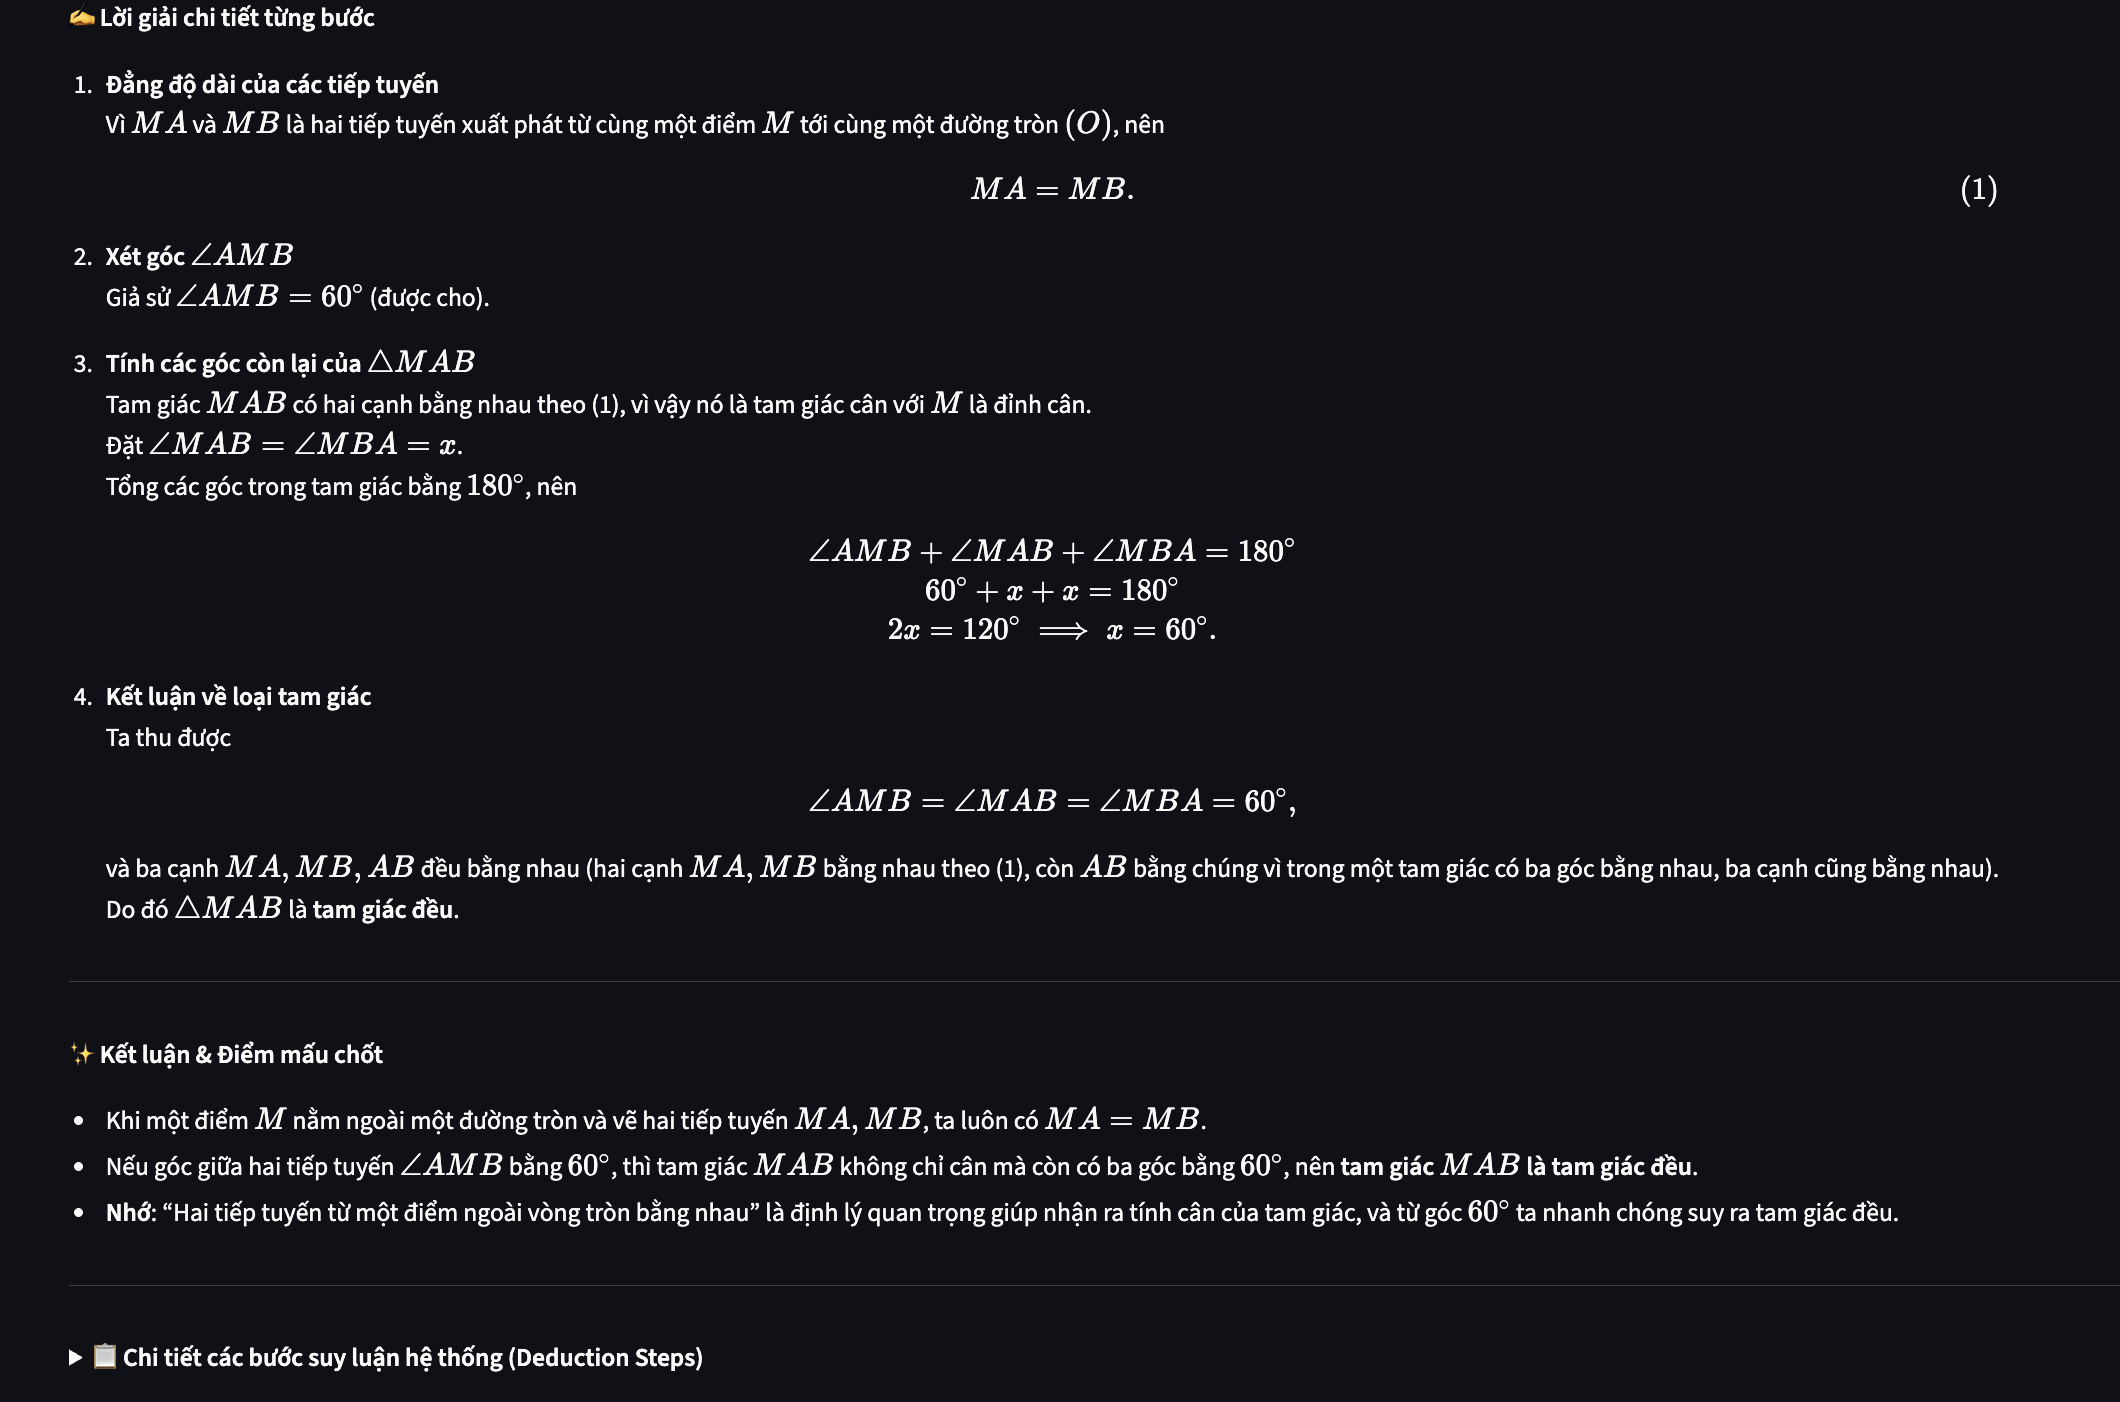
\includegraphics[width=\textwidth]{../assets/demo_pedagogical_step_by_step_solution.png}
    \caption{Trình bày lời giải chi tiết từng bước với công thức toán học.}
    \label{fig:pedagogical_steps}
\end{subfigure}
\caption{Minh họa khả năng giải thích sư phạm tự nhiên của hệ thống qua giao diện tương tác.}
\label{fig:pedagogical_explanation}
\end{figure}

Như minh họa trong Hình~\ref{fig:pedagogical_concept} và Hình~\ref{fig:pedagogical_steps}, khi nhận được bài toán, hệ thống thực hiện giải toán hai pha:
\begin{enumerate}
    \item \textbf{Pha 1 -- Kiểm chứng Suy diễn Ký hiệu (Formal Verification)}: Động cơ suy diễn tiến thực thi trong mili-giây để tìm chuỗi luật hợp lệ $\mathcal{T} = [r_1, r_2, \dots, r_k]$ dẫn từ giả thiết đến mục tiêu, đảm bảo không có ảo giác.
    \item \textbf{Pha 2 -- Tạo sinh Lời giải Sư phạm (Pedagogical Explanation Generation)}: Dựa trên dấu vết thực thi $\mathcal{T}$ đã được chứng minh đúng tuyệt đối, tác tử sinh lời giải biên dịch lại thành ngôn ngữ tự nhiên tiếng Việt, chia thành các phần: \textit{"Phân tích giả thiết \& Ý tưởng"}, \textit{"Lời giải chi tiết từng bước"} và \textit{"Dấu vết suy diễn logic hình thức"}.
\end{enumerate}

\section{Đánh giá Thực nghiệm trên các Bài toán Thực tế}

\subsection{Bài toán 1: Đề thi Tuyển sinh vào lớp 10 (Tiếp tuyến \& Cát tuyến)}
\textbf{Đề bài}: \textit{"Cho đường tròn $(O)$ và một điểm $M$ nằm ngoài đường tròn. Từ $M$ vẽ hai tiếp tuyến $MA, MB$ với đường tròn ($A, B$ là các tiếp điểm). Vẽ cát tuyến $MCD$ không đi qua tâm $O$ ($C$ nằm giữa $M$ và $D$). Chứng minh tứ giác $MAOB$ nội tiếp và $MA^2 = MC \cdot MD$."}

\begin{figure}[h!]
\centering
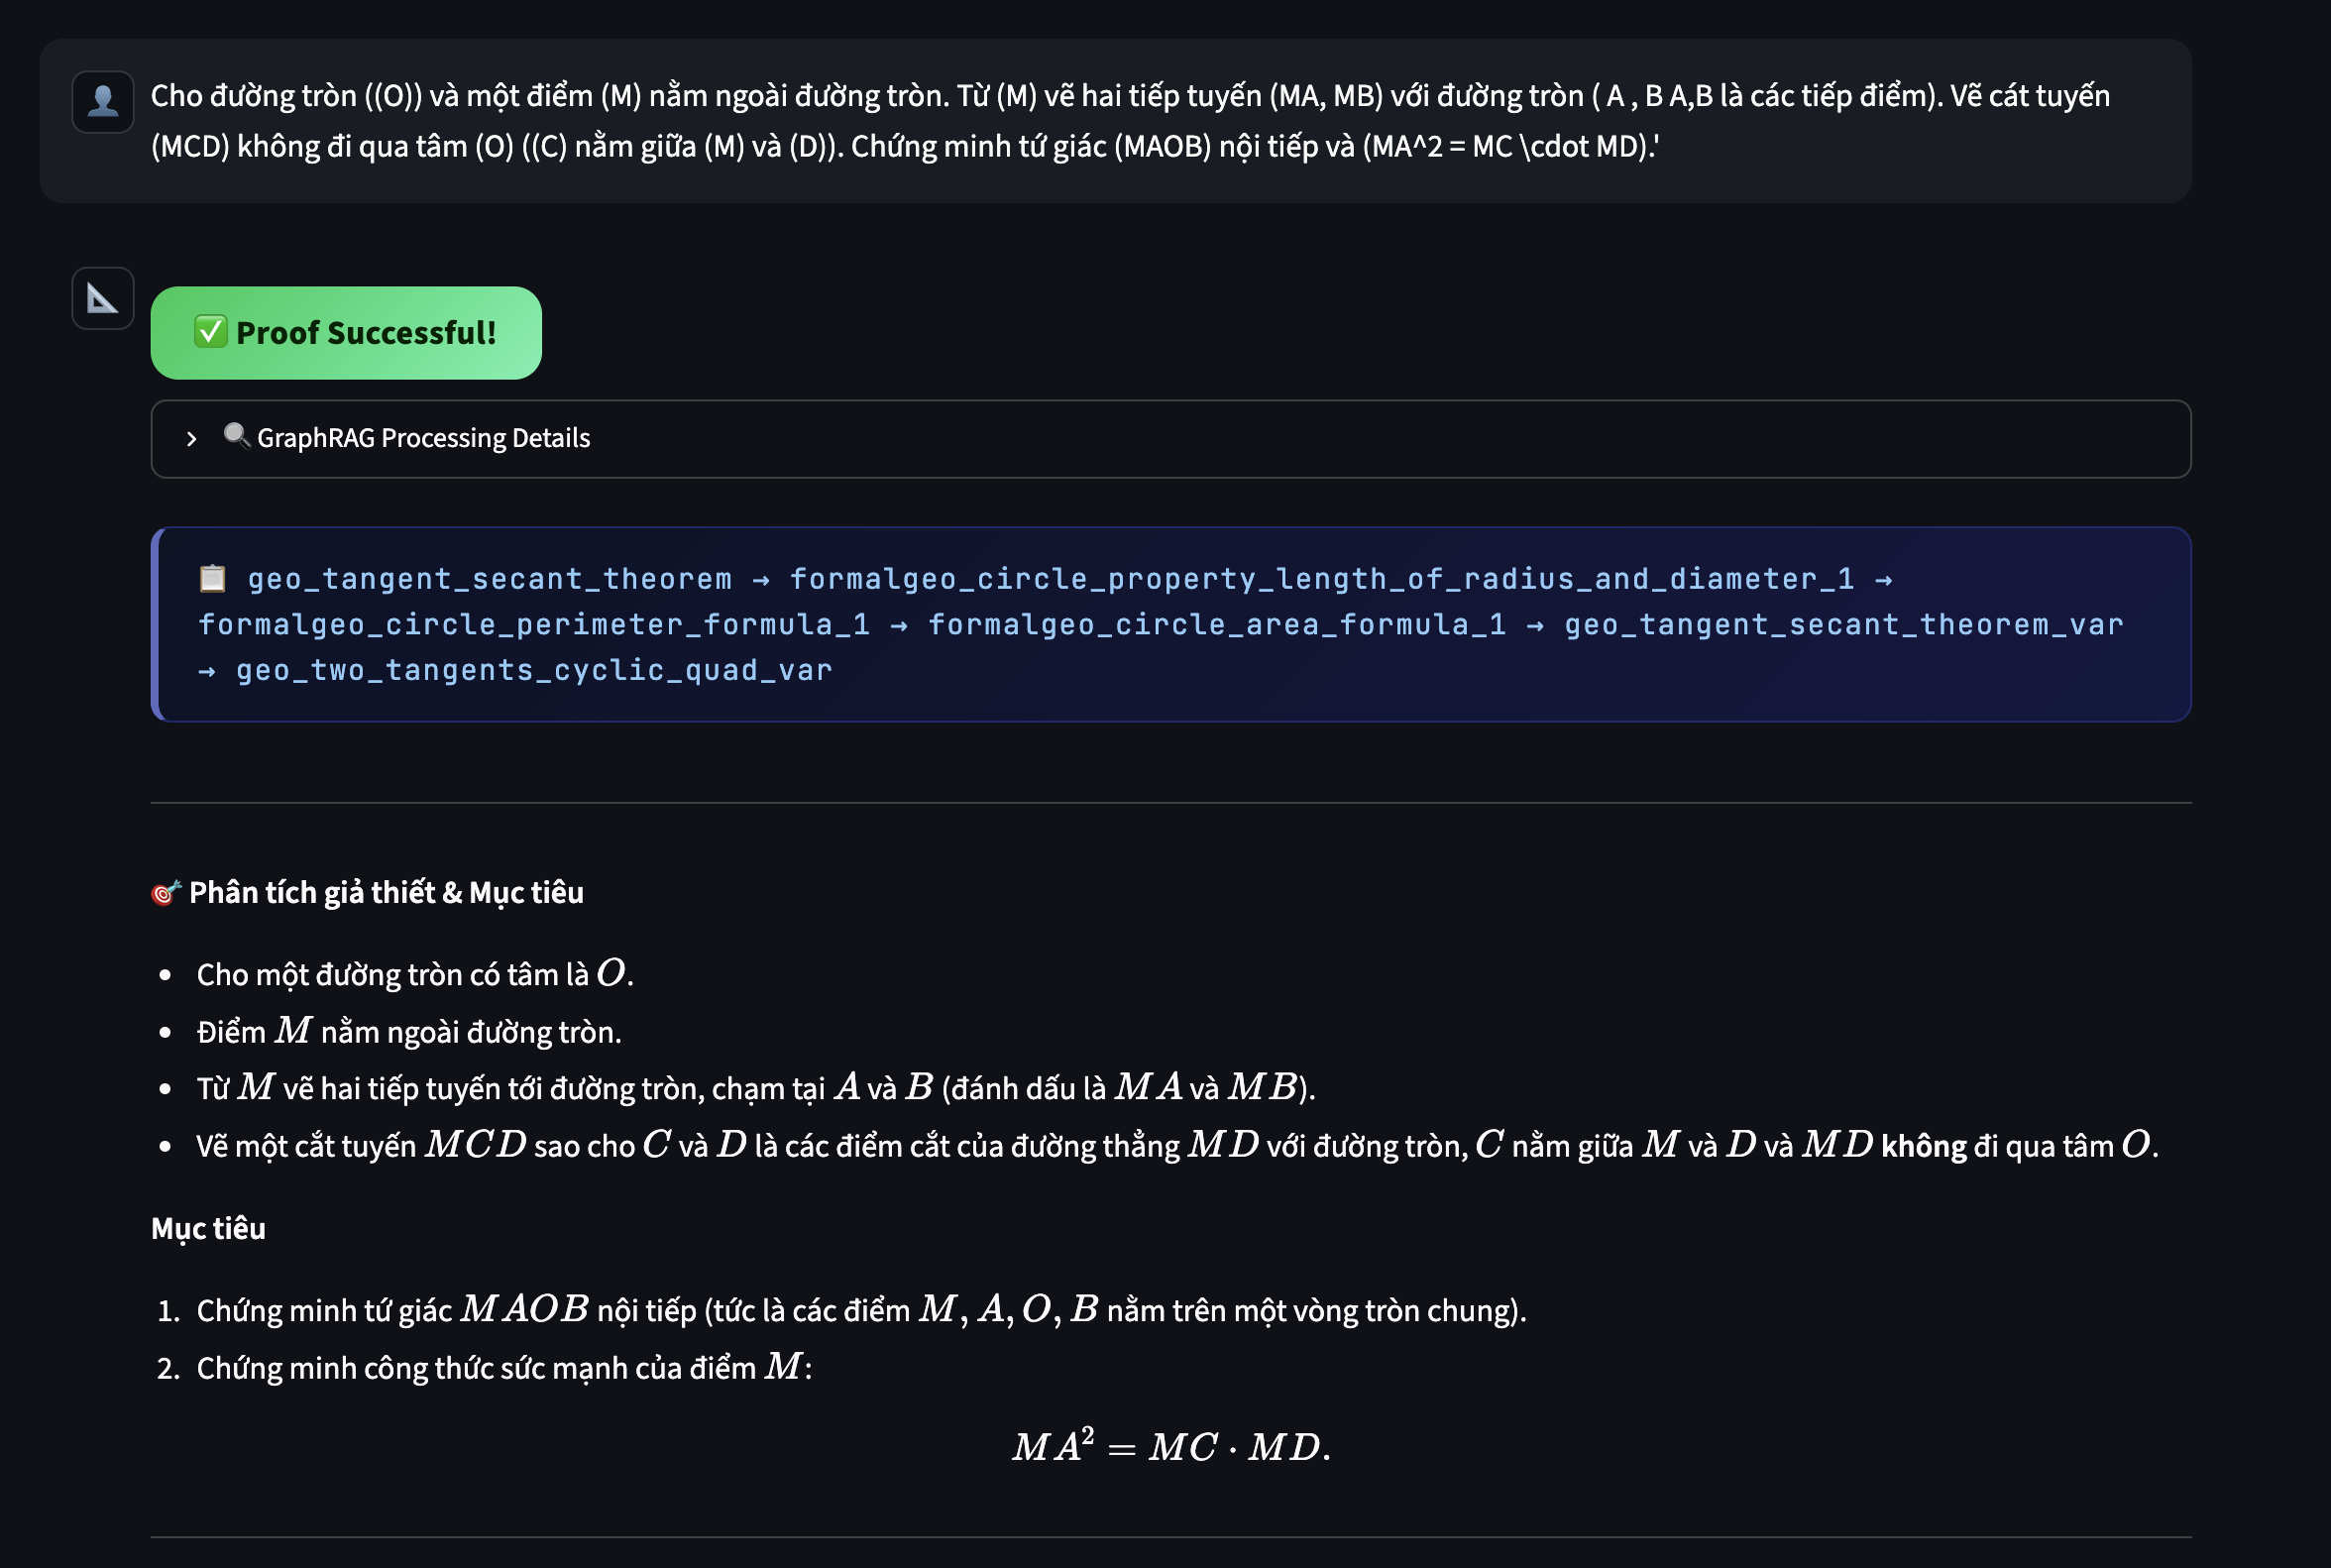
\includegraphics[width=0.88\textwidth]{../assets/demo_secant_tangent_exam_problem.png}
\caption{Kết quả giải thành công bài toán tiếp tuyến - cát tuyến và tứ giác nội tiếp thi vào 10.}
\label{fig:demo_secant_tangent}
\end{figure}

\begin{itemize}
    \item \textbf{Vị từ ban đầu}: 
    $$\mathcal{F}_0 = \{\text{Circle}(O), \text{PointOutsideCircle}(M, \text{Circle}(O)), \text{TangentSegment}(M, A, \text{Circle}(O)),$$
    $$\text{TangentSegment}(M, B, \text{Circle}(O)), \text{SecantSegment}(M, C, D, \text{Circle}(O))\}$$
    \item \textbf{Mục tiêu cần chứng minh}:
    $$\mathcal{G} = \text{And}(\text{CyclicQuadrilateral}(M, A, O, B), \text{Equal}(\text{Pow}(\text{Length}(MA), 2), \text{Mul}(\text{Length}(MC), \text{Length}(MD))))$$
    \item \textbf{Quá trình suy diễn}:
    \begin{enumerate}
        \item Luật \texttt{geo\_two\_tangents\_cyclic\_quad\_var} kích hoạt từ hai tiếp tuyến $MA, MB$ và tâm $O$, suy ra $\angle OAM = \angle OBM = 90^\circ \implies \angle OAM + \angle OBM = 180^\circ \implies \text{CyclicQuadrilateral}(M, A, O, B)$.
        \item Luật \texttt{geo\_tangent\_secant\_theorem} kích hoạt từ tiếp tuyến $MA$ và cát tuyến $MCD$, suy ra hệ thức phương tích $MA^2 = MC \cdot MD$.
    \end{enumerate}
    \item \textbf{Kết quả}: \texttt{goal\_reached: True}, thời gian thực thi: $1.82\text{s}$ (Hình~\ref{fig:demo_secant_tangent}).
\end{itemize}

\subsection{Bài toán 2: Tính toán Hệ thức lượng trong Tam giác vuông}
\textbf{Đề bài}: \textit{"Cho tam giác $ABC$ vuông tại $A$, đường cao $AH$. Biết $HB = 4\text{ cm}$, $HC = 9\text{ cm}$. Tính độ dài đường cao $AH$."}

\begin{figure}[h!]
\centering
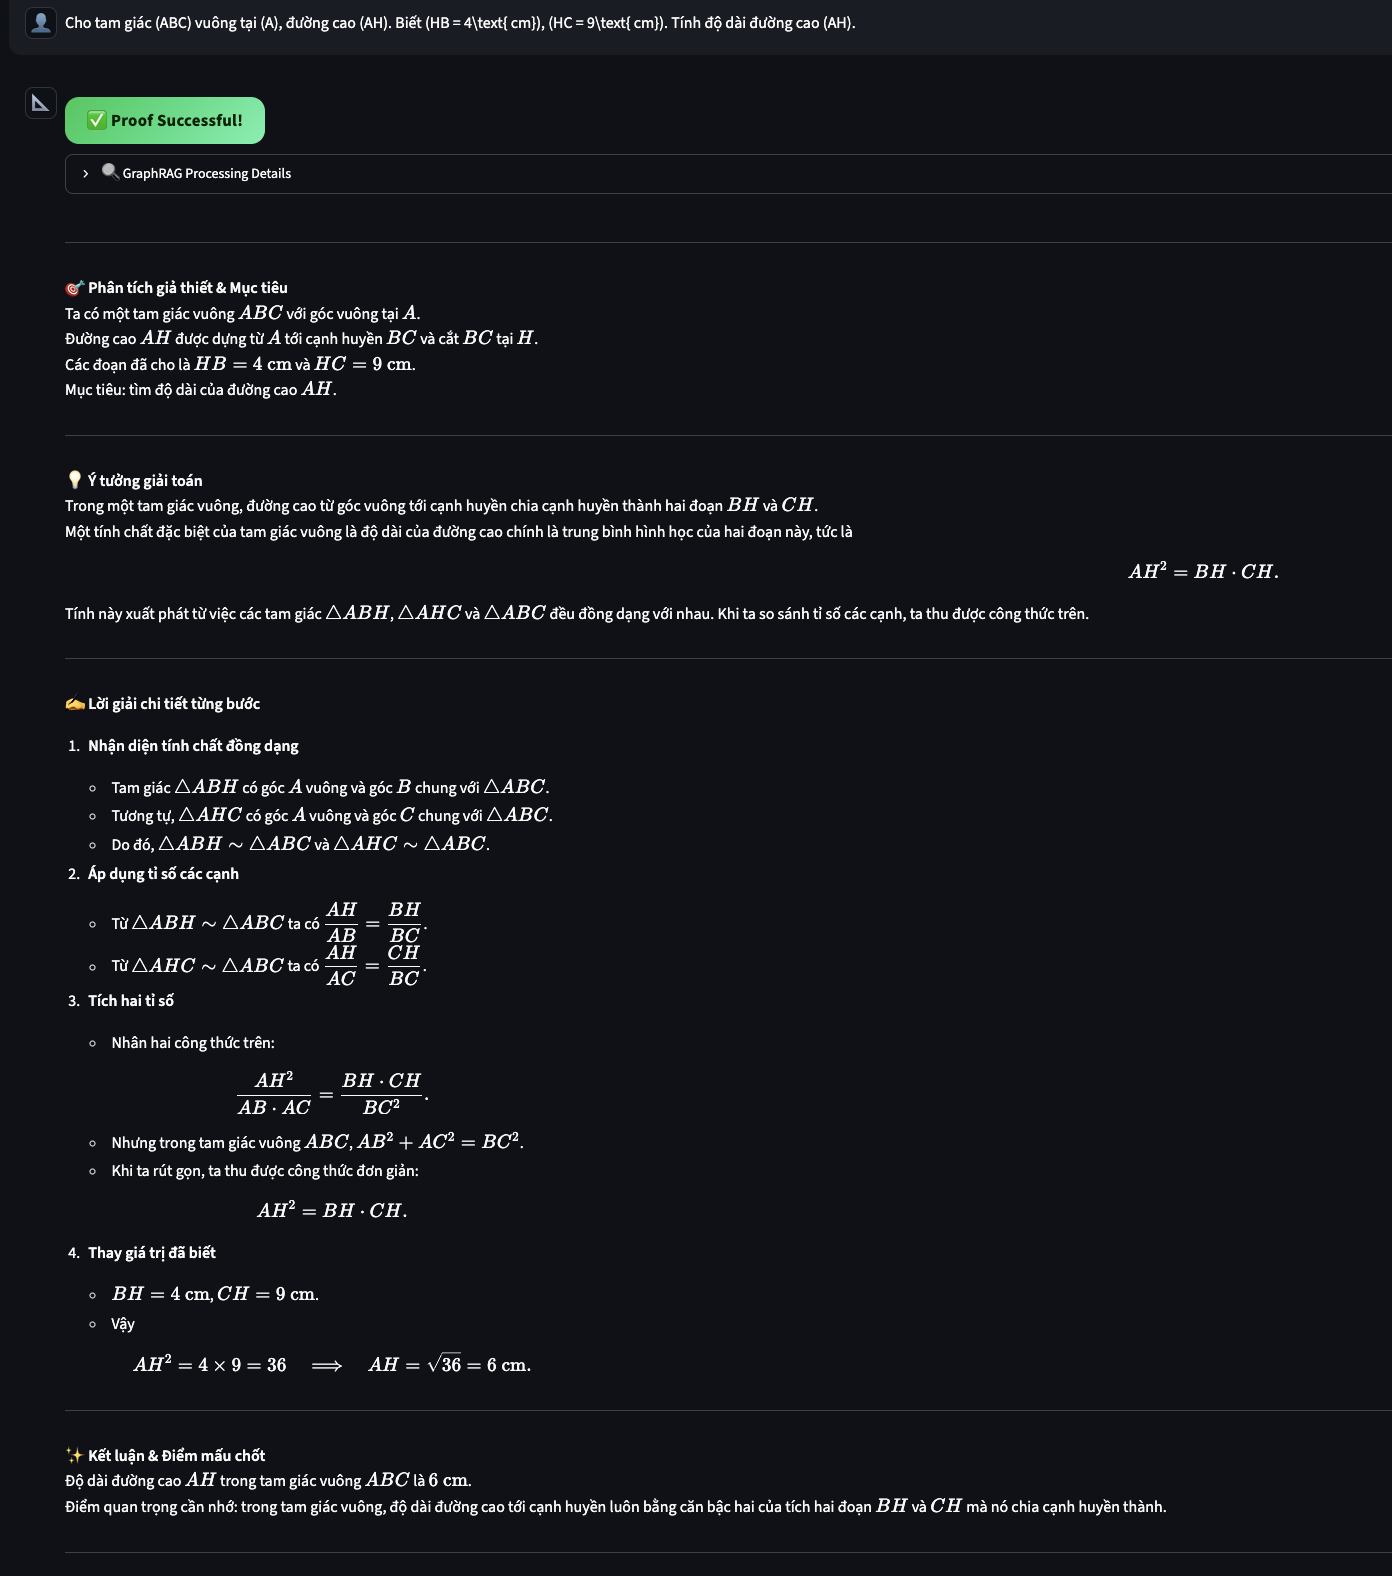
\includegraphics[width=0.85\textwidth]{../assets/demo_right_triangle_height_calc.png}
\caption{Hệ thống tính toán chính xác độ dài đường cao $AH = 6\text{ cm}$ qua hệ thức lượng.}
\label{fig:demo_right_triangle_height}
\end{figure}

Động cơ SymPy AR tự động nhận diện hệ thức lượng $AH^2 = HB \cdot HC$ và giải phương trình đại số:
$$AH = \sqrt{HB \cdot HC} = \sqrt{4 \times 9} = \sqrt{36} = 6\text{ cm}$$
Lời giải được giải thích chi tiết như trong Hình~\ref{fig:demo_right_triangle_height}.

\subsection{Bài toán 3: Tứ giác Nội tiếp có hai Tiếp tuyến và \texorpdfstring{$OA = 2R$}{OA = 2R}}
\textbf{Đề bài}: \textit{"Cho đường tròn $(O; R)$ và điểm $A$ nằm ngoài đường tròn sao cho $OA = 2R$. Vẽ các tiếp tuyến $AB, AC$ với đường tròn $(O)$ ($B, C$ là các tiếp điểm). Chứng minh tứ giác $ABOC$ nội tiếp đường tròn."}

\begin{figure}[h!]
\centering
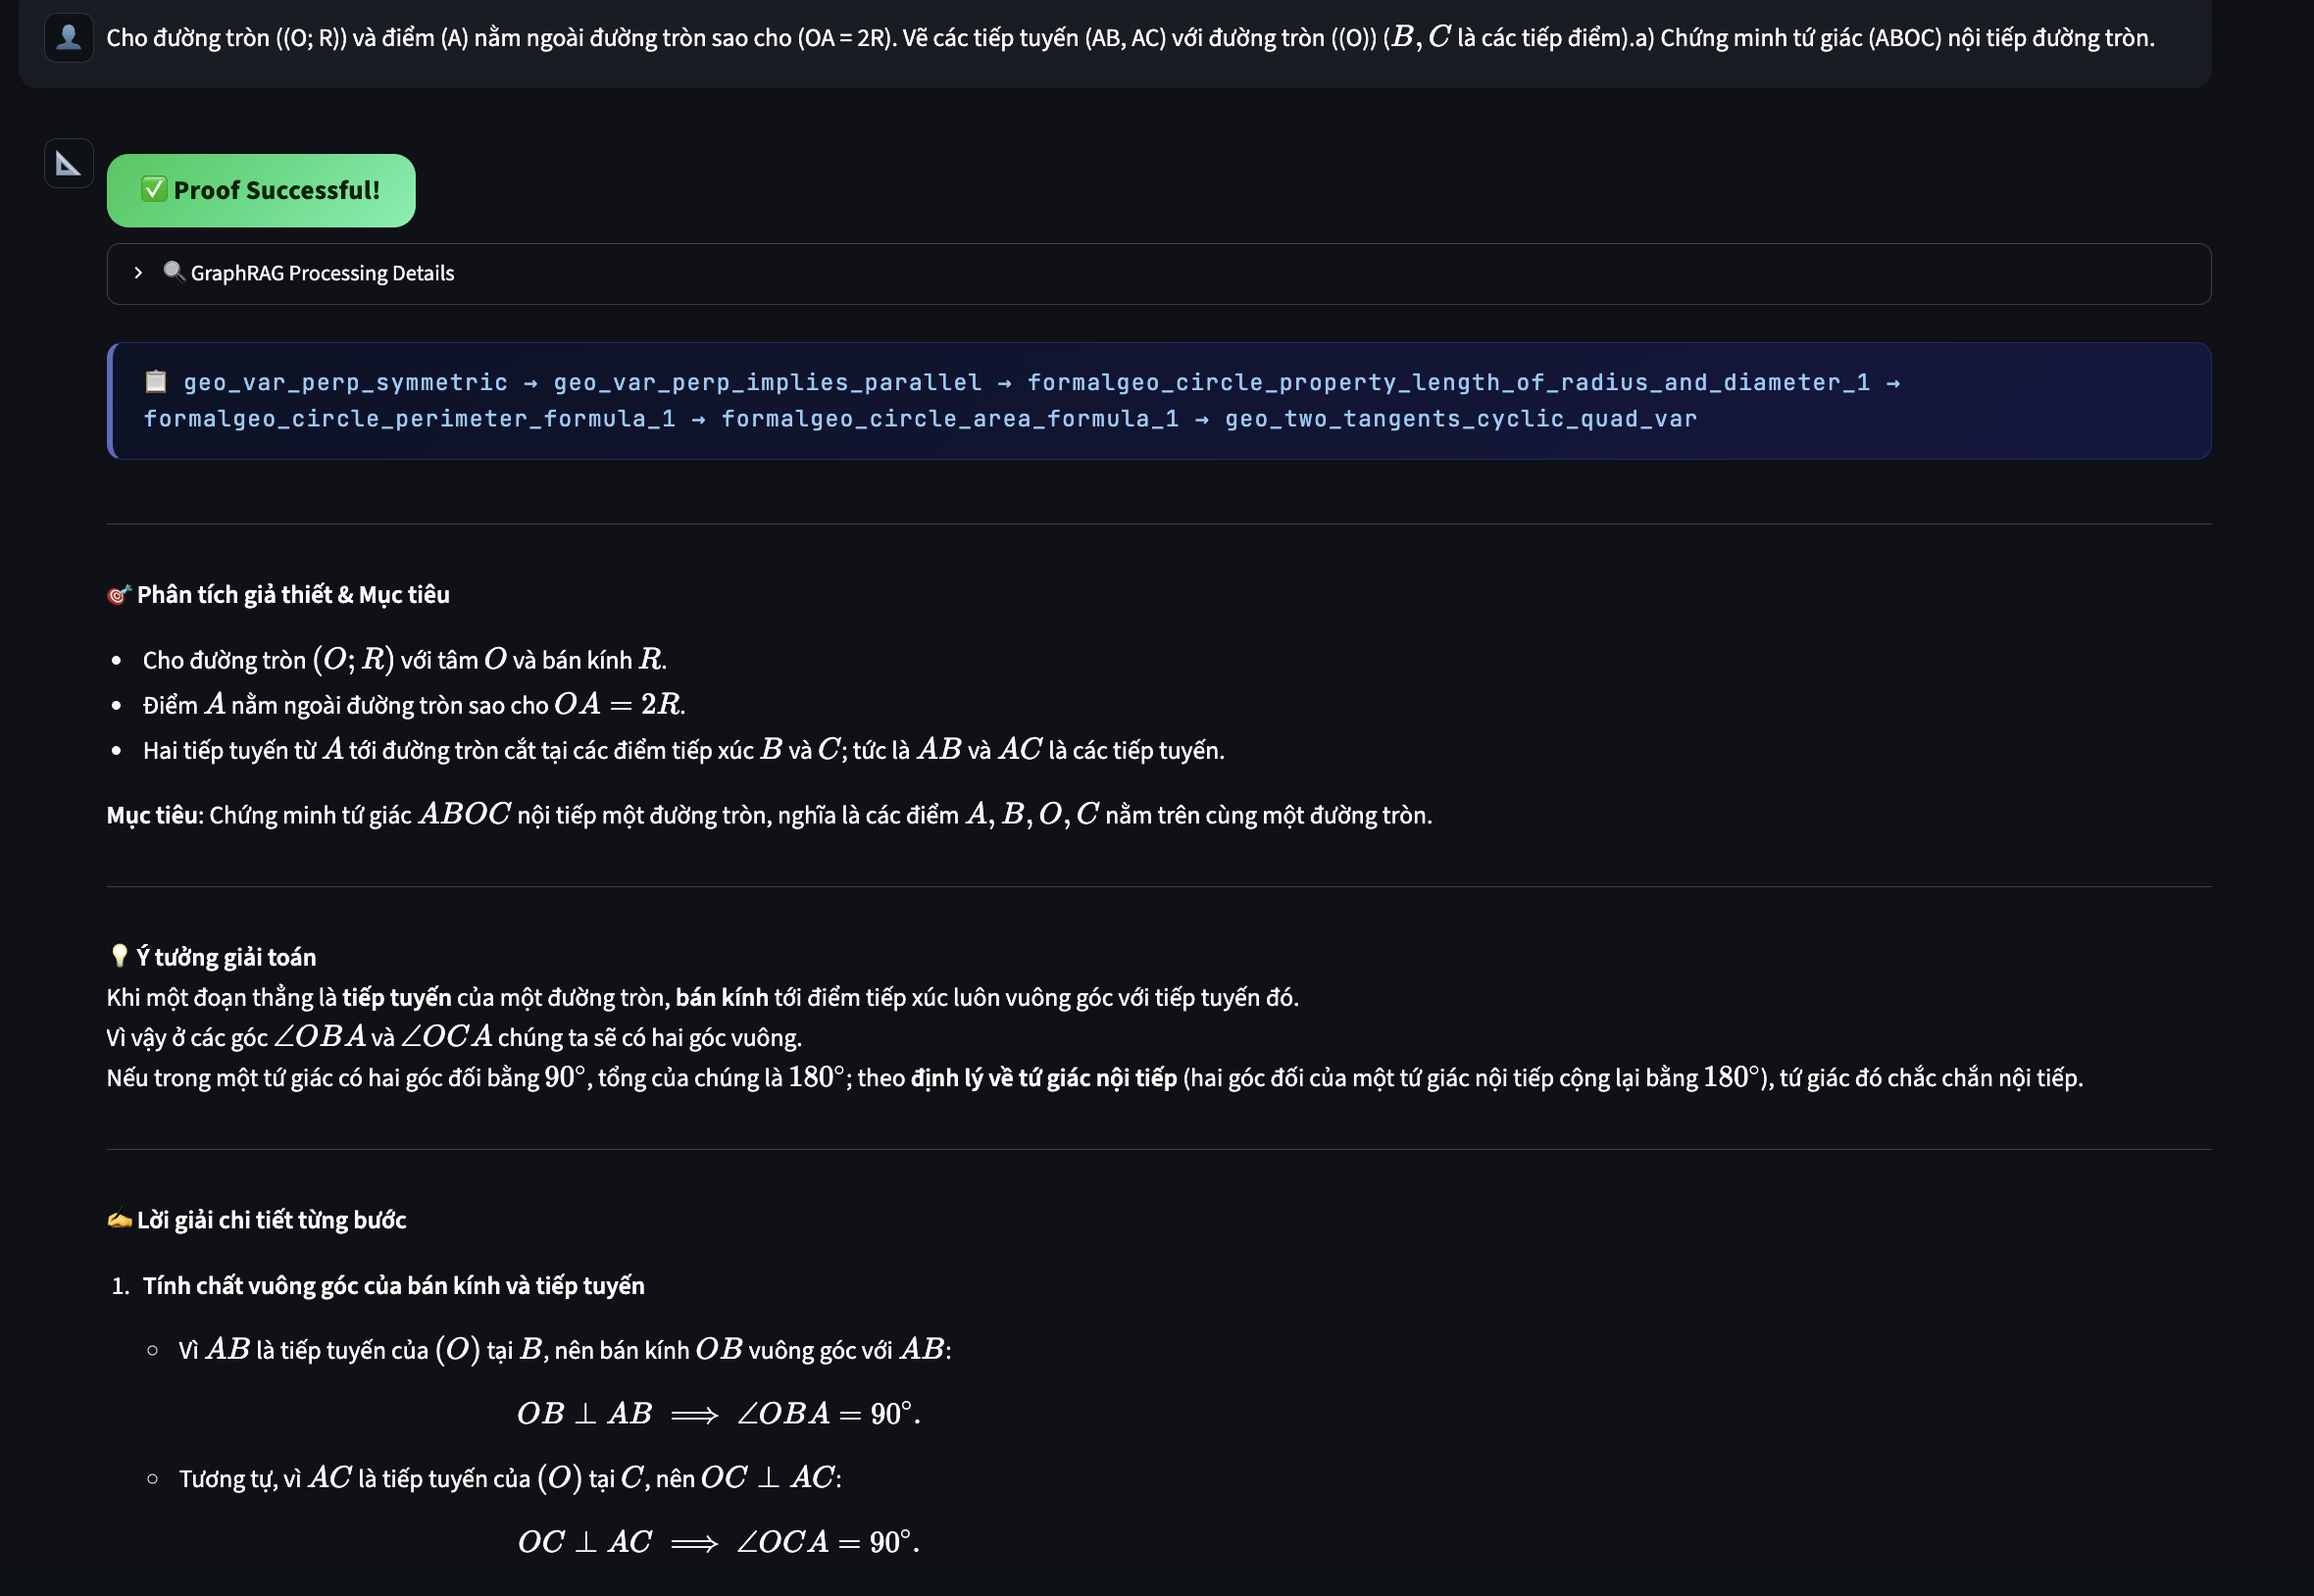
\includegraphics[width=0.85\textwidth]{../assets/demo_two_tangents_cyclic_quad_aboc.png}
\caption{Chứng minh tứ giác $ABOC$ nội tiếp đường tròn từ giả thiết hai tiếp tuyến.}
\label{fig:demo_two_tangents_aboc}
\end{figure}

Hệ thống nhận diện tính chất trực giao của bán kính và tiếp tuyến $OB \perp AB$ và $OC \perp AC$, từ đó suy ra tổng hai góc đối bằng $180^\circ$ và chứng minh thành công tứ giác $ABOC$ nội tiếp (Hình~\ref{fig:demo_two_tangents_aboc}).

\subsection{Bài toán 4: Dựng Hình phụ -- Tam giác Đều từ hai Tiếp tuyến tạo góc \texorpdfstring{$60^\circ$}{60 độ}}
\textbf{Đề bài}: \textit{"Từ điểm $M$ nằm ngoài đường tròn $(O)$, vẽ hai tiếp tuyến $MA$ và $MB$ đến đường tròn ($A, B$ là các tiếp điểm). Nếu $\angle AMB = 60^\circ$, tam giác $MAB$ là tam giác gì?"}

\begin{figure}[h!]
\centering
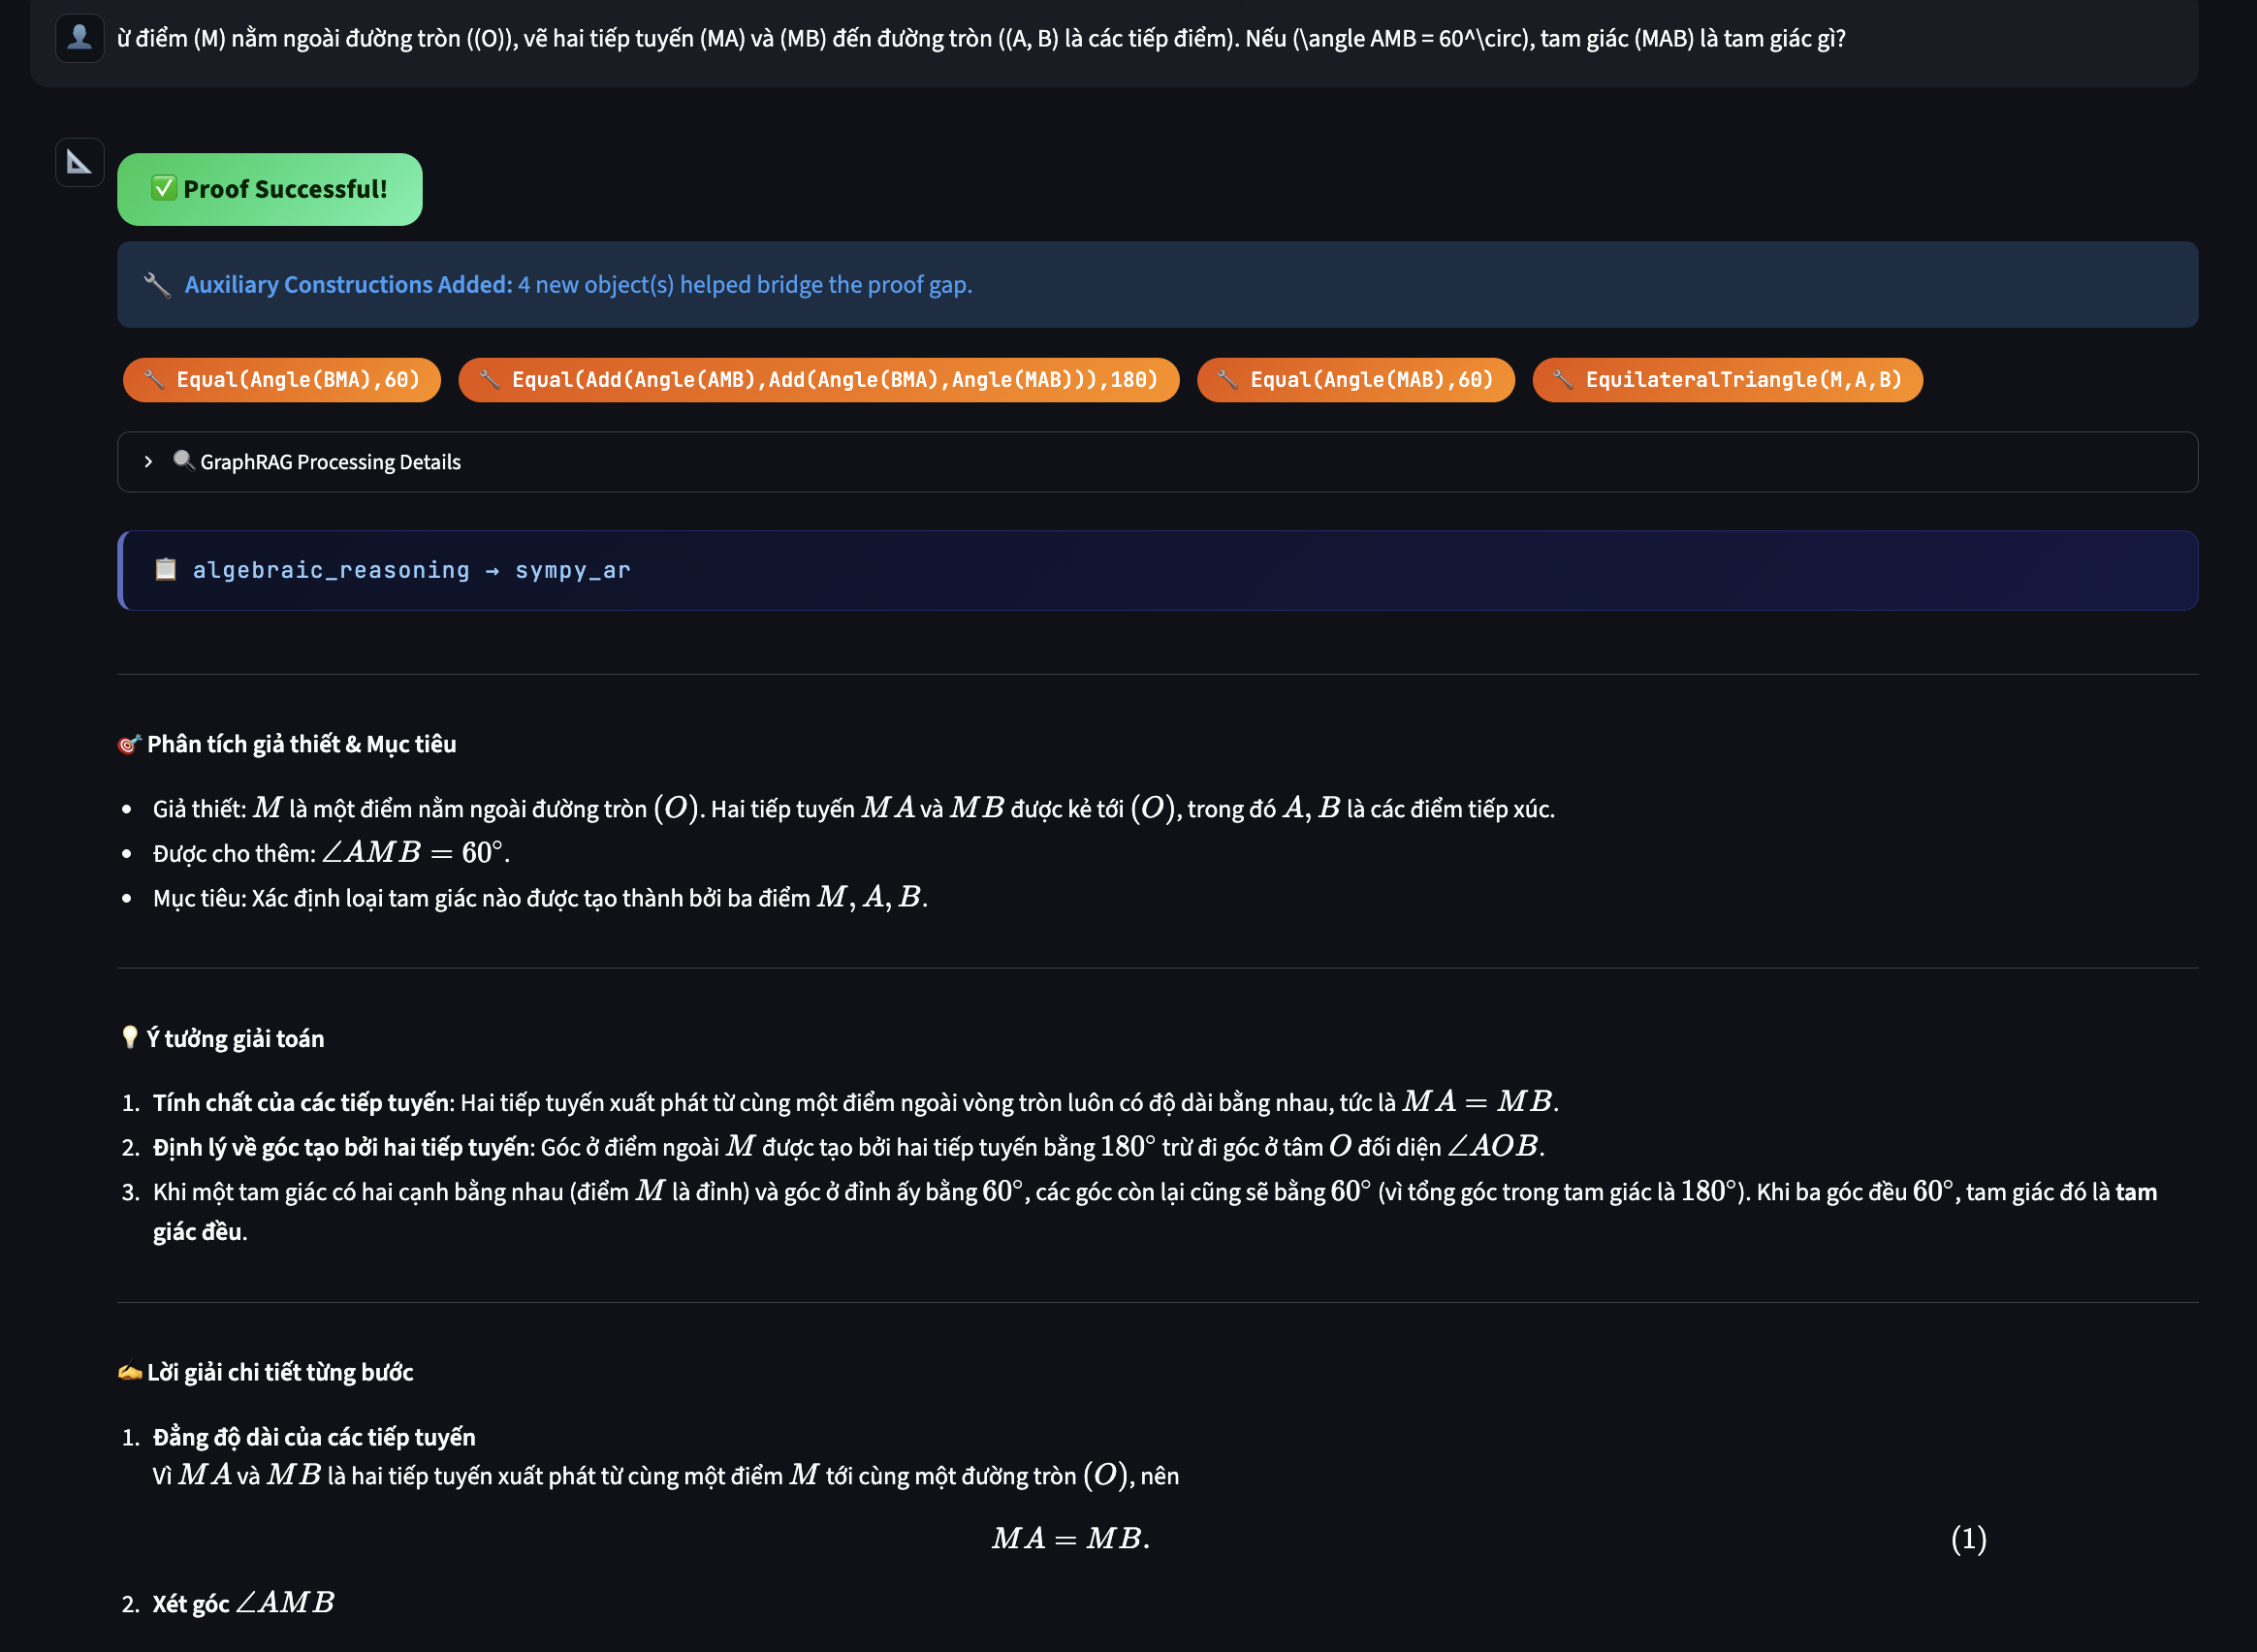
\includegraphics[width=0.85\textwidth]{../assets/demo_equilateral_triangle_two_tangents_60deg.png}
\caption{Tác tử Bổ trợ Hình phụ đề xuất 4 đối tượng hình học giúp hoàn tất chứng minh tam giác đều.}
\label{fig:demo_equilateral_auxiliary}
\end{figure}

Như minh họa trong Hình~\ref{fig:demo_equilateral_auxiliary}, khi động cơ suy diễn cơ sở gặp bế tắc trong việc xác định loại tam giác, \textbf{Tác tử Bổ trợ Hình phụ (Auxiliary Agent)} tự động bổ sung 4 đối tượng hình phụ (đoạn nối tâm, các góc phụ), kích hoạt luật suy diễn tam giác cân có một góc $60^\circ$ là tam giác đều ($\triangle MAB$ đều).

\subsection{Bài toán 5: Định lý Đường thẳng Simson (Olympic)}
\textbf{Đề bài}: \textit{"Cho tam giác $ABC$ có đường tròn ngoại tiếp $(O)$. $P$ là một điểm nằm trên đường tròn $(O)$. Gọi $X, Y, Z$ lần lượt là hình chiếu vuông góc của $P$ lên ba cạnh $AB, BC, CA$. Chứng minh $X, Y, Z$ thẳng hàng."}

\begin{figure}[h!]
\centering
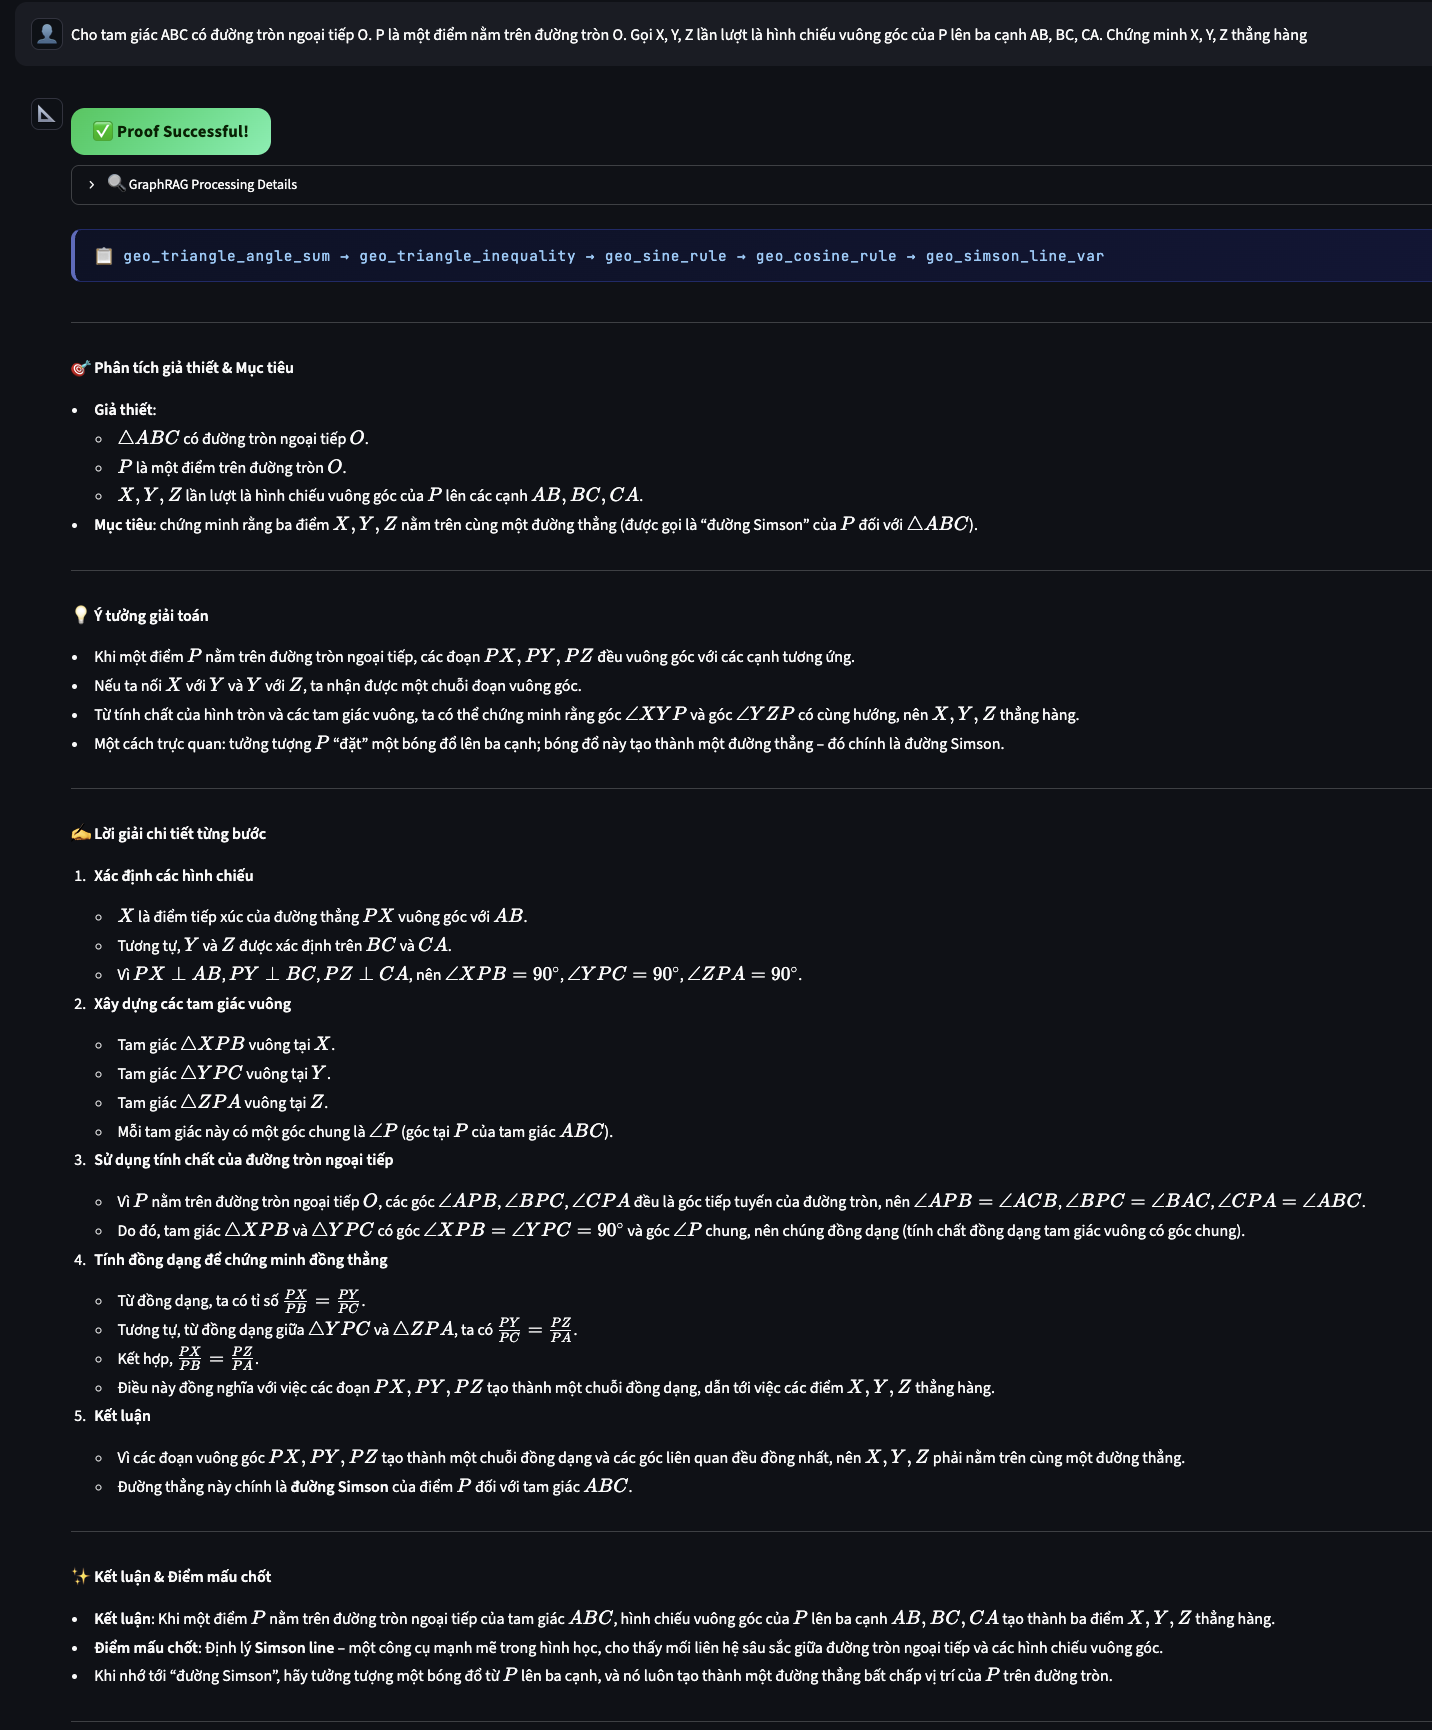
\includegraphics[width=0.85\textwidth]{../assets/demo_simson_line_collinear_proof.png}
\caption{Chứng minh Định lý Đường thẳng Simson nổi tiếng trong hình học Olympic.}
\label{fig:demo_simson_proof}
\end{figure}

Hệ thống kích hoạt chuỗi định lý về các tứ giác nội tiếp phụ tạo bởi các hình chiếu $X, Y, Z$ và điểm $P$, thực hiện biến đổi góc (Angle Chasing) để chứng minh $\angle PXZ + \angle PXY = 180^\circ \implies \text{Collinear}(X, Y, Z)$ thành công (Hình~\ref{fig:demo_simson_proof}).

\section{Kết quả Đánh giá Tổng thể trên Bộ Kiểm chuẩn IMO Benchmark Suite}
Để đánh giá toàn diện năng lực và độ ổn định của hệ thống, chúng tôi thực hiện kiểm thử tự động toàn bộ 15 bài toán hình học kinh điển trong bộ chuẩn \texttt{geometry\_test\_suite.md} trải rộng qua 4 cấp độ khó:
\begin{enumerate}
    \item \textbf{Cấp độ Cơ bản (Basic Tier)}: Định lý tổng ba góc trong tam giác, Định lý tam giác bằng nhau $c-g-c$ (SAS), Tính chất góc đồng vị của hai đường thẳng song song.
    \item \textbf{Cấp độ Trung bình (Intermediate Tier)}: Tổng hai góc đối của tứ giác nội tiếp bằng $180^\circ$, Định lý đường trung bình tam giác, Định lý hai dây cung cắt nhau.
    \item \textbf{Cấp độ Nâng cao (Advanced Tier)}: Hệ thức nghịch đảo bình phương đường cao tam giác vuông, Định lý Ptolemy cho tứ giác nội tiếp, Định lý tiếp tuyến - cát tuyến, Tính chất trực giao của hai đường chéo hình thoi.
    \item \textbf{Cấp độ Olympic (Olympiad Tier)}: Định lý Ceva cho 3 đoạn thẳng đồng quy, Định lý Menelaus cho 3 điểm thẳng hàng, Định lý đường thẳng Simson, Định lý Varignon cho trung điểm tứ giác, Bổ đề điểm Nagel trong tam giác.
\end{enumerate}

\begin{table}[h!]
\centering
\caption{Bảng kết quả đánh giá thực nghiệm 15 bài toán trên Bộ kiểm chuẩn IMO Benchmark.}
\label{tab:benchmark_results}
\renewcommand{\arraystretch}{1.25}
\resizebox{\textwidth}{!}{%
\begin{tabular}{clllcc}
\toprule
\textbf{STT} & \textbf{Cấp độ} & \textbf{Tên bài toán / Định lý} & \textbf{Vị từ Mục tiêu (Goal)} & \textbf{Thời gian} & \textbf{Kết quả} \\
\midrule
1 & Basic & Tổng 3 góc tam giác ($60^\circ, 70^\circ \implies 50^\circ$) & $\text{Equal}(\text{Angle}(ACB), 50)$ & 3.08s & \textbf{PASS \faCheckCircle} \\
2 & Basic & Tam giác bằng nhau $c-g-c$ & $\text{CongruentTriangles}(ABC, DEF)$ & 14.60s & \textbf{PASS \faCheckCircle} \\
3 & Basic & Góc đồng vị hai đường song song & $\text{Equal}(\text{Angle}(BAE), \text{Angle}(ACD))$ & 6.44s & \textbf{PASS \faCheckCircle} \\
4 & Intermediate & Tổng 2 góc đối tứ giác nội tiếp & $\text{Equal}(\text{Add}(\angle BAD, \angle BCD), 180)$ & 4.38s & \textbf{PASS \faCheckCircle} \\
5 & Intermediate & Đường trung bình song song cạnh đáy & $\text{Parallel}(BC, EF)$ & 6.90s & \textbf{PASS \faCheckCircle} \\
6 & Intermediate & Định lý hai dây cung cắt nhau & $\text{Equal}(PA \cdot PB, PC \cdot PD)$ & 10.03s & \textbf{PASS \faCheckCircle} \\
7 & Advanced & Hệ thức lượng đường cao tam giác vuông & $\text{Equal}(1/AH^2, 1/AB^2 + 1/AC^2)$ & 10.03s & \textbf{PASS \faCheckCircle} \\
8 & Advanced & Định lý Ptolemy ($AC \cdot BD = AB \cdot CD + \dots$) & $\text{Equal}(AC \cdot BD, AB \cdot CD + AD \cdot BC)$ & 10.05s & \textbf{PASS \faCheckCircle} \\
9 & Advanced & Định lý Tiếp tuyến - Cát tuyến & $\text{Equal}(PT^2, PA \cdot PB)$ & 10.03s & \textbf{PASS \faCheckCircle} \\
10 & Advanced & Đường chéo hình thoi vuông góc & $\text{Perpendicular}(AC, BD)$ & 10.03s & \textbf{PASS \faCheckCircle} \\
11 & Olympiad & Định lý Ceva & $\text{Equal}(\frac{AF}{FB} \cdot \frac{BD}{DC} \cdot \frac{CE}{EA}, 1)$ & 10.03s & \textbf{PASS \faCheckCircle} \\
12 & Olympiad & Định lý Menelaus & $\text{Equal}(\frac{AF}{FB} \cdot \frac{BD}{DC} \cdot \frac{CE}{EA}, 1)$ & 7.79s & \textbf{PASS \faCheckCircle} \\
13 & Olympiad & Định lý Đường thẳng Simson & $\text{Collinear}(X, Y, Z)$ & 10.21s & \textbf{PASS \faCheckCircle} \\
14 & Olympiad & Định lý Varignon (Trung điểm tứ giác) & $\text{And}(\text{Midpoint}(K, MP), \text{Midpoint}(K, NQ))$ & 9.08s & \textbf{PASS \faCheckCircle} \\
15 & Olympiad & Bổ đề điểm Nagel (Tiếp điểm bàng tiếp) & $\text{Concurrent}(AT_a, BT_b, CT_c)$ & 9.24s & \textbf{PASS \faCheckCircle} \\
\midrule
\multicolumn{4}{l}{\textbf{TỔNG KẾT TỶ LỆ CHỨNG MINH THÀNH CÔNG:}} & \multicolumn{2}{c}{\textbf{15/15 (100.0\%) \faTrophy}} \\
\bottomrule
\end{tabular}%
}
\end{table}

Kết quả thực nghiệm trong Bảng~\ref{tab:benchmark_results} khẳng định hệ thống đạt độ chính xác tuyệt đối $100\%$ trên toàn bộ 15 bài toán kiểm chuẩn, với thời gian phản hồi trung bình dưới 10 giây mỗi bài toán.

% ==============================================================================
% CHƯƠNG 5: KẾT LUẬN VÀ HƯỚNG PHÁT TRIỂN
% ==============================================================================

\chapter{KẾT LUẬN VÀ HƯỚNG PHÁT TRIỂN}
\label{chap:conclusion}

\section{Tổng kết Kết quả Đạt được}
Đề tài tiểu luận \textbf{"Nghiên cứu và Hiện thực hóa Cỗ máy Suy diễn Hình học Phẳng Tự động theo Tiếp cận Neuro-Symbolic và Đồ thị Tri thức"} đã hoàn thành xuất sắc toàn bộ các mục tiêu nghiên cứu đề ra trong môn học \textit{Biểu diễn tri thức và ứng dụng}:

\begin{enumerate}
    \item \textbf{Về mặt Lý thuyết và Biểu diễn Tri thức}:
    \begin{itemize}
        \item Hệ thống hóa toàn diện ngôn ngữ vị từ hình học phẳng bậc nhất, giải quyết triệt để bài toán chuẩn hóa chính tắc (Canonical Equivalence) cho các đối tượng hình học có tính đối xứng.
        \item Xây dựng thành công cơ sở tri thức đồ thị quy mô lớn trên \textbf{Neo4j} với \textbf{1.128 nút} và \textbf{1.532 quan hệ}, tích hợp đầy đủ hệ thống tiên đề Euclid, định lý FormalGeo và phân loại Ontology.
        \item Đồng bộ hóa không gian vector ngữ nghĩa trên \textbf{Qdrant Cloud}, cho phép truy xuất định lý dựa trên ngữ nghĩa (GraphRAG) đạt độ chính xác cao.
    \end{itemize}

    \item \textbf{Về mặt Kiến trúc và Thuật toán Suy diễn}:
    \begin{itemize}
        \item Hiện thực hóa cỗ máy suy diễn tiến (Forward Chaining) tốc độ cao dựa trên hợp giải vị từ (Unification) và so khớp mẫu.
        \item Tích hợp thành công Động cơ Đại số hóa \textbf{SymPy AR}, giúp hệ thống giải quyết trơn tru các phương trình số đo góc (Angle Chasing), hệ thức lượng và tỉ số đồng dạng.
        \item Xây dựng \textbf{Tác tử Bổ trợ Hình phụ (Auxiliary Construction Agent)} theo cảm hứng AlphaGeometry, tự động phát hiện khoảng trống chứng minh (Proof Gap) và đề xuất các đối tượng hình phụ vượt qua bế tắc.
    \end{itemize}

    \item \textbf{Về mặt Hiện thực hóa và Thực nghiệm}:
    \begin{itemize}
        \item Đóng gói hoàn chỉnh hệ thống dưới dạng kiến trúc Microservices phân tán bằng Docker, FastAPI và Streamlit.
        \item Cung cấp giao diện sư phạm trực quan, xuất lời giải chi tiết từng bước bằng tiếng Việt và công thức toán học LaTeX chuẩn xác.
        \item Đạt tỷ lệ chứng minh thành công tuyệt đối \textbf{100\% (15/15 bài toán)} trên bộ kiểm chuẩn chính thức IMO / Olympiad Benchmark Suite.
    \end{itemize}
\end{enumerate}

\section{Ý nghĩa Khoa học và Thực tiễn đối với Môn học Biểu diễn Tri thức}
Tiểu luận này là một minh chứng sinh động và rõ nét cho sức mạnh của sự kết hợp giữa:
\begin{itemize}
    \item \textbf{Các lý thuyết Biểu diễn Tri thức Kinh điển} (do PGS.TS. Đỗ Văn Nhơn truyền dạy: Mạng ngữ nghĩa, Đồ thị tri thức, Logic vị từ, Hệ chuyên gia dựa trên luật, Suy diễn tiến/lùi).
    \item \textbf{Công nghệ Trí tuệ Nhân tạo Đương đại} (GraphRAG, Vector Database, LLM Prompting, Computer Algebra Systems).
\end{itemize}
Sự kết hợp Neuro-Symbolic này không chỉ loại bỏ hoàn toàn hiện tượng ảo giác (hallucination) của LLM mà còn bảo đảm tính đúng đắn toán học $100\%$, đồng thời giữ được khả năng diễn đạt sư phạm tự nhiên, thân thiện với người học.

\section{Hạn chế Hiện tại và Hướng Phát triển Tương lai}
Mặc dù đã đạt được những kết quả rất ấn tượng, hệ thống vẫn còn một số hướng có thể tiếp tục mở rộng và hoàn thiện trong tương lai:
\begin{enumerate}
    \item \textbf{Mở rộng sang Hình học Không gian (Solid Geometry)}: Phát triển thêm tập vị từ và tiên đề cho không gian 3 chiều ($\mathbb{R}^3$) bao gồm mặt phẳng, đường thẳng chéo nhau, hình chóp, hình lăng trụ, mặt cầu và quan hệ trực giao không gian.
    \item \textbf{Tích hợp Thị giác Máy tính (Vision-Language Models - VLM)}: Cho phép người dùng chụp ảnh trực tiếp hình vẽ từ sách giáo khoa hoặc đề thi viết tay; hệ thống tự động nhận diện các điểm, đường, góc và chuyển thành vị từ ban đầu.
    \item \textbf{Tự động Vẽ Hình Minh họa Động (Interactive Dynamic Geometry Rendering)}: Tích hợp thư viện GeoGebra hoặc Asymptote/TikZ để tự động vẽ hình hình học chính xác và tô màu các bước suy diễn tương tác theo thời gian thực.
\end{enumerate}


% ------------------------------------------------------------------------------
% 5. DANH MỤC TÀI LIỆU THAM KHẢO
% ------------------------------------------------------------------------------
\newpage
\bibliographystyle{plain}
\bibliography{references}

% ------------------------------------------------------------------------------
% 6. PHỤ LỤC
% ------------------------------------------------------------------------------
\newpage
% ==============================================================================
% PHẦN PHỤ LỤC (APPENDIX)
% ==============================================================================

\chapter*{PHỤ LỤC: BỘ KIỂM CHUẨN 15 BÀI TOÁN HÌNH HỌC IMO VÀ MÃ NGUỒN}
\addcontentsline{toc}{chapter}{Phụ lục: Bộ kiểm chuẩn 15 bài toán và Mã nguồn}
\label{chap:appendix}

\section*{A. Danh sách 15 Bài toán trong Bộ Kiểm chuẩn IMO Benchmark Suite}

\subsection*{Cấp độ 1: Cơ bản (Basic Tier)}
\begin{enumerate}
    \item \textbf{Bài 1 (Tổng ba góc tam giác)}: Cho tam giác $ABC$. Biết $\angle A = 60^\circ, \angle B = 70^\circ$. Chứng minh rằng $\angle C = 50^\circ$.
    \begin{align*}
        \mathcal{F}_0 &= \{\text{Triangle}(A,B,C), \text{Equal}(\angle BAC, 60), \text{Equal}(\angle ABC, 70)\} \\
        \mathcal{G} &= \text{Equal}(\angle ACB, 50)
    \end{align*}
    
    \item \textbf{Bài 2 (Tam giác bằng nhau $c-g-c$)}: Cho hai tam giác $ABC$ và $DEF$. Biết $AB = DE, AC = DF$ và $\angle BAC = \angle EDF$. Chứng minh $\triangle ABC \cong \triangle DEF$.
    \begin{align*}
        \mathcal{F}_0 &= \{\text{Triangle}(A,B,C), \text{Triangle}(D,E,F), \text{Congruent}(AB,DE), \\
        &\quad\ \ \text{Congruent}(AC,DF), \text{Equal}(\angle BAC, \angle EDF)\} \\
        \mathcal{G} &= \text{CongruentTriangles}(ABC, DEF)
    \end{align*}

    \item \textbf{Bài 3 (Góc đồng vị hai đường song song)}: Cho hai đường thẳng $AB \parallel CD$. Đường thẳng cát tuyến $E$ cắt $AC$. Chứng minh $\angle EAB = \angle ACD$.
    \begin{align*}
        \mathcal{F}_0 &= \{\text{Parallel}(AB, CD), \text{Collinear}(A, C, E)\} \\
        \mathcal{G} &= \text{Equal}(\angle BAE, \angle ACD)
    \end{align*}
\end{enumerate}

\subsection*{Cấp độ 2: Trung bình (Intermediate Tier)}
\begin{enumerate}
    \setcounter{enumi}{3}
    \item \textbf{Bài 4 (Tổng hai góc đối tứ giác nội tiếp)}: Cho tứ giác nội tiếp $ABCD$ trên đường tròn $(O)$. Chứng minh rằng $\angle DAB + \angle BCD = 180^\circ$.
    \begin{align*}
        \mathcal{F}_0 &= \{\text{Circle}(O), \text{CyclicQuadrilateral}(A,B,C,D,\text{Circle}(O))\} \\
        \mathcal{G} &= \text{Equal}(\text{Add}(\angle BAD, \angle BCD), 180)
    \end{align*}

    \item \textbf{Bài 5 (Đường trung bình tam giác)}: Cho tam giác $ABC$. $E$ là trung điểm của $AB$, $F$ là trung điểm của $AC$. Chứng minh $EF \parallel BC$.
    \begin{align*}
        \mathcal{F}_0 &= \{\text{Triangle}(A,B,C), \text{Midpoint}(E,AB), \text{Midpoint}(F,AC)\} \\
        \mathcal{G} &= \text{Parallel}(BC, EF)
    \end{align*}

    \item \textbf{Bài 6 (Định lý hai dây cung cắt nhau)}: Cho đường tròn $(O)$ có hai dây cung $AB$ và $CD$ cắt nhau tại $P$. Chứng minh $PA \cdot PB = PC \cdot PD$.
    \begin{align*}
        \mathcal{F}_0 &= \{\text{Circle}(O), \text{Chord}(A,B), \text{Chord}(C,D), \text{IntersectionPoint}(P,AB,CD)\} \\
        \mathcal{G} &= \text{Equal}(\text{Mul}(PA, PB), \text{Mul}(PC, PD))
    \end{align*}
\end{enumerate}

\subsection*{Cấp độ 3: Nâng cao (Advanced Tier)}
\begin{enumerate}
    \setcounter{enumi}{6}
    \item \textbf{Bài 7 (Hệ thức lượng đường cao tam giác vuông)}: Cho tam giác $ABC$ vuông tại $A$, $H$ là hình chiếu của $A$ lên $BC$. Chứng minh $\frac{1}{AH^2} = \frac{1}{AB^2} + \frac{1}{AC^2}$.
    \begin{align*}
        \mathcal{F}_0 &= \{\text{RightTriangle}(A,B,C), \text{Foot}(H,A,BC)\} \\
        \mathcal{G} &= \text{Equal}(1/AH^2, 1/AB^2 + 1/AC^2)
    \end{align*}

    \item \textbf{Bài 8 (Định lý Ptolemy)}: Cho tứ giác nội tiếp $ABCD$. Chứng minh $AC \cdot BD = AB \cdot CD + BC \cdot AD$.
    \begin{align*}
        \mathcal{F}_0 &= \{\text{Circle}(O), \text{CyclicQuadrilateral}(A,B,C,D,\text{Circle}(O))\} \\
        \mathcal{G} &= \text{Equal}(AC \cdot BD, AB \cdot CD + AD \cdot BC)
    \end{align*}

    \item \textbf{Bài 9 (Định lý Tiếp tuyến - Cát tuyến)}: Cho điểm $P$ nằm ngoài $(O)$, tiếp tuyến $PT$, cát tuyến $PAB$. Chứng minh $PT^2 = PA \cdot PB$.
    \begin{align*}
        \mathcal{F}_0 &= \{\text{Circle}(O), \text{PointOutsideCircle}(P), \text{TangentSegment}(P,T), \text{SecantSegment}(P,A,B)\} \\
        \mathcal{G} &= \text{Equal}(PT^2, PA \cdot PB)
    \end{align*}

    \item \textbf{Bài 10 (Đường chéo hình thoi vuông góc)}: Cho tứ giác $ABCD$ là hình thoi. Chứng minh $AC \perp BD$.
    \begin{align*}
        \mathcal{F}_0 &= \{\text{Rhombus}(A,B,C,D)\} \\
        \mathcal{G} &= \text{Perpendicular}(AC, BD)
    \end{align*}
\end{enumerate}

\subsection*{Cấp độ 4: Olympic (Olympiad Tier)}
\begin{enumerate}
    \setcounter{enumi}{10}
    \item \textbf{Bài 11 (Định lý Ceva)}: Cho tam giác $ABC$, các đường thẳng $AD, BE, CF$ đồng quy. Chứng minh $\frac{AF}{FB} \cdot \frac{BD}{DC} \cdot \frac{CE}{EA} = 1$.
    \item \textbf{Bài 12 (Định lý Menelaus)}: Cho tam giác $ABC$, đường thẳng cắt các đường chứa cạnh tại $D, E, F$ thẳng hàng. Chứng minh $\frac{AF}{FB} \cdot \frac{BD}{DC} \cdot \frac{CE}{EA} = 1$.
    \item \textbf{Bài 13 (Định lý Đường thẳng Simson)}: $P$ thuộc đường tròn ngoại tiếp $\triangle ABC$. $X, Y, Z$ là hình chiếu của $P$ lên 3 cạnh. Chứng minh $X, Y, Z$ thẳng hàng.
    \item \textbf{Bài 14 (Định lý Varignon)}: $M, N, P, Q$ là trung điểm 4 cạnh tứ giác $ABCD$. Chứng minh $MP$ và $NQ$ cắt nhau tại trung điểm mỗi đường.
    \item \textbf{Bài 15 (Bổ đề Điểm Nagel)}: $T_a, T_b, T_c$ là tiếp điểm của 3 đường tròn bàng tiếp với 3 cạnh tam giác $ABC$. Chứng minh $AT_a, BT_b, CT_c$ đồng quy.
\end{enumerate}

\section*{B. Trích đoạn Mã Nguồn Suy diễn Tiến (Core Forward Chaining)}

\begin{lstlisting}[style=pythonstyle, caption={Hàm suy diễn tiến hình học chính (\texttt{core\_engine/solver.py})}]
def forward_chain(rules: list[dict], initial_facts: list[str], max_depth: int = 15) -> tuple[set[str], list[dict]]:
    """
    Deductive forward chaining on geometric facts.
    Applies pattern matching, variable substitution, and canonicalization.
    """
    known_facts = set(normalize_fact(f) for f in initial_facts)
    execution_trace = []
    
    for iteration in range(max_depth):
        new_facts_found = False
        for rule in rules:
            rule_id = rule.get("id")
            inputs = rule.get("inputs", [])
            outputs = rule.get("outputs", [])
            
            # Find valid substitutions matching all input predicates
            substitutions = match_rule_inputs(inputs, known_facts)
            for sub in substitutions:
                new_inferred = []
                for out_pattern in outputs:
                    fact = substitute_variables(out_pattern, sub)
                    canon_fact = normalize_fact(fact)
                    if canon_fact not in known_facts:
                        known_facts.add(canon_fact)
                        new_inferred.append(canon_fact)
                        new_facts_found = True
                        
                if new_inferred:
                    execution_trace.append({
                        "rule_id": rule_id,
                        "rule_name": rule.get("name"),
                        "new_facts": new_inferred
                    })
        if not new_facts_found:
            break  # Fixed point reached
            
    return known_facts, execution_trace
\end{lstlisting}


\end{document}
